\documentclass[11pt]{article}

%\usepackage{setspace}
%\documentclass[final,leqno]{siamltex}
\usepackage{smoothing_paper}



\usepackage[section]{placeins}
\usepackage{tabularx,ragged2e,booktabs,caption}

%%%%%%%%%%%%%%%%%%%%%%%%%%%%%%%%chiheb commands

\interfootnotelinepenalty=10000
%%%%%%%%%%%%%%%%%
\newcommand{\ie}{\emph{i.e.}}
\newcommand{\eg}{\emph{e.g.}}
\newcommand{\cf}{\emph{cf.}}
\newcommand{\prob}[1]{\mathrm{P}\left(#1\right)}
\newcommand{\expt}[1]{\mathrm{E}\left[#1\right]}
\newcommand{\expth}[1]{\hat{\mathrm{E}}\left[#1\right]}



\newcommand{\rset}{\mathbb{R}}
\newcommand{\nset}{\mathbb{N}}
\newcommand{\zset}{\mathbb{Z}}



\newcommand{\PERIOD}{.}
\newcommand{\COMMA}{,}
\newcommand{\BIGSPACE}{\,\,\,\,\,\,\,}



\newcommand{\Ordo}[1]{{\mathcal{O}}\left(#1\right)}
\newcommand{\ordo}[1]{{o}\left(#1\right)}

%%%%%%%%%%%%%%%%%%%%%%%%%%%%%%%%%%%%%%%%%%%%%%%%%%%%%%%%%%%%%%%%%%%%%%%%
%%
%% DO WE RELLY NEED THE FOLLOWING??

%%  new margin
%%%%%%%%%%%%%%%%%%%%%%%%%%%%%%%%%%%%%%%%%%%
\pagestyle{plain}                                                      %%
%%%%%%%%%% EXACT 1in MARGINS %%%%%%%                                   %%
\setlength{\textwidth}{6.5in}     %%                                   %%
\setlength{\oddsidemargin}{0in}   %%   
\setlength{\evensidemargin}{0in}  %%        
\setlength{\textheight}{8.5in}    %%       
\setlength{\topmargin}{-0.2in}    %%   
\setlength{\headheight}{0in}      %%    
\setlength{\headsep}{0in}         %%                   
\setlength{\footskip}{.5in}       %%                       
%%%%%%%%%%%%%%%%%%%%%%%%%%%%%%%%%%%%                                   %%
\newcommand{\required}[1]{\section*{\hfil #1\hfil}}                    %%
\renewcommand{\refname}{\hfil References Cited\hfil}                   %%

\def\SMALLSKIP{\smallskip}
\def\MEDSKIP{\medskip}
\def\BIGSKIP{\bigskip}

%%
%%%%%%%%%%%%%%%%%%%%%%%%%%%%%%%%%%%%%%%%%%%%%%%%%%%%%%%%%%%%%%%%%%%%%

\makeatletter
\def\BState{\State\hskip-\ALG@thistlm}
\makeatother



%%%%%%%%%%%%%%%%%%%%%%%%%%%%%%%%%%%%%%%%

\title{Hierarchical adaptive sparse  grids for option pricing under the rough Bergomi model} 



\author{Christian Bayer\thanks{
 Weierstrass Institute for Applied Analysis and Stochastics (WIAS),
 Berlin, Germany.}
        \and Chiheb Ben Hammouda\thanks{King Abdullah University of Science and Technology (KAUST), Computer, Electrical and Mathematical Sciences \& Engineering Division (CEMSE), Thuwal $23955-6900$, Saudi Arabia ({\tt chiheb.benhammouda@kaust.edu.sa}).} 
\and  Raul Tempone\thanks{King Abdullah University of Science and Technology (KAUST), Computer, Electrical and Mathematical Sciences \& Engineering Division (CEMSE), Thuwal $23955-6900$, Saudi Arabia ({\tt raul.tempone@kaust.edu.sa}).} \thanks{Alexander von Humboldt Professor in Mathematics for Uncertainty Quantification, RWTH Aachen University, Germany.}}

%\doublespacing
\begin{document}
\maketitle

\begin{abstract}
	One of the recent rough volatility models that showed a promising potential in quantitative finance   is the rough Bergomi model, introduced in \cite{bayer2016pricing}. This new model exhibits consistent results with the empirical fact of implied volatility surfaces being essentially time-invariant, and  ability to capture the term structure of skew observed in equity markets. In the absence of analytical European option pricing methods for the model,  the prevalent option is to use Monte Carlo (MC) simulation for efficient pricing. We design a novel alternative hierarchical approach, based on adaptive sparse grids quadrature, specifically  multi-index stochastic collocation (MISC) as in  \cite{haji2016multi}, coupled with Brownian bridge construction and Richardson extrapolation. This hierarchical method demonstrates substantial computational gains with respect to the standard Monte Carlo method, assuming a sufficiently small error tolerance in the price estimates, across different parameter constellations.

\

\textbf{Keywords} Rough volatility, Monte Carlo, multi-index stochastic collocation, Brownian bridge construction, Richardson extrapolation.

\textbf{2010 Mathematics Subject Classification} 	91G60, 	91G20, 65C05, 65D30, 65D32.  
\end{abstract}






%\pagestyle{myheadings}
\thispagestyle{plain}

\setcounter{tocdepth}{1}


 \section{Introduction}
In many  applications, the quantity of interest is usually expressed as 
\begin{equation}\label{eq:QoI}
\expt{g(X)},
\end{equation}
where  $X$ is a certain stochastic process and $g$ is an observable of the state  process $X$.

For instance, in quantitative finance,   the price of an option on an underlying $S$ can typically- disregarding discounting-be expressed as \eqref{eq:QoI}, for some (payoff) function $g$ on $S$ and the expectation operator $E$ induced by the appropriate pricing measure. 

Approximating  \eqref{eq:QoI} is usually challenging due to a combination of two complications
\begin{itemize}
\item $X$ often takes values in a high-dimensional state space.  For instance in computational finance the reason for the high dimensionality may be the time-discretization of a stochastic differential equation,  path dependence of the option (i.e., $S$ is actually a path of an asset price, not the value at a specific time), a large number of underlying assets, or others.
\item The payoff function $g$ is  not smooth. In fact,  in many cases, the  integrand contains either kinks or jumps. For instance, in the context of option pricing,  an option is normally considered worthless if the value falls below a predetermined strike price.  A kink  (discontinuity in the gradients) is present when the payoff function is  continuous such as the case of digital option with payoff function $g$ being the indicator function. On the other hand, a jump  exists  when the function is discontinuous itself, for instance, this is the case when approximating densities and thus $g$ is represented by the Dirac Delta function in that case. 
\end{itemize}
There are mainly two approaches for approximating \eqref{eq:QoI}
\begin{enumerate}
\item The first approach treats problem \eqref{eq:QoI} as a stochastic problem and relies  on Monte Carlo (MC) methods (standard MC, Multilevel Monte Carlo (MLMC) \cite{giles2015multilevel}, etc \dots) to approximate the expectation in \eqref{eq:QoI}.  Although, standard Monte Carlo complexity  is insensitive to both the dimension and the regularity of $g$, it has a very slow rate of convergence. On the other hand, MLMC, which is based on hierarchical representation of the expectation and has a better complexity than standard MC,  is highly affected by the low regularity of $g$, due to its effect on i) the strong convergence rate and ii) the kurtosis. For instance, when $g$ is  either the Dirac delta or the indicator functions, standard MLMC  fail or not has the optimal performance, due to the singularity present in $g$, that causes  i) high variance, ii) low strong convergence rate and iii) high kurtosis for the MLMC estimator. 

In the literature, few works tried to address this issue. For instance, Avikainen in \cite{avikainen2009irregular}, and Giles, Higham, and Mao in \cite{giles2009analysing} used MLMC for such a task without smoothing and obtained bad performance for MLMC estimator.  On the other hand, a second approach  was suggested in  \cite{giles2008improved,giles2013numerical}, that used implicit smoothing based on the use of conditional expectations. There are two potential issues  with this second approach: i) In general cases, one may have dynamics where it is not easy to derive an  analytic expression for the conditional expectation and ii) This approach used a higher order scheme, that is the Milstein scheme, to improve the strong order of convergence, and consequently the complexity of the MLMC estimator. Such a scheme becomes very computationally expensive for higher dimensional dynamics. Different non smooth payoff functions were considered in \cite{giles2008improved,giles2013numerical} (Asian, barrier, digital)  but the only considered dynamics were under the GBM model. Finally, in \cite{giles2015multilevel}, the authors suggested a different approach based on parametric smoothing.  In fact, they carefully constructed a regularized version of the QoI, based on a  regularization parameter that depends on the weak and strong convergence rates and also  the tolerance requirement.  This approach, despite offering better performance for the MLMC estimator and a better setting for theoretical analysis, it has the practical disadvantage consisting in the difficulty of generalizing it to cases where there is no prior knowledge of the  convergence rates (that is they need to be estimated numerically), and also for each error tolerance, a new  regularization parameter needs to be computed. Note also that all the numerical examples in \cite{giles2015multilevel} were based on the GBM dynamics.

In this work, we address a similar problem and  propose an alternative approach that is  based on numerical smoothing. The numerical smoothing idea is based on i) finding lines or areas of discontinuity using root finding algorithms such Newton algorithm, ii)  employing suitable transformations of the integration domain, and iii) a pre-integration (smoothing) step with respect to the dimension containing the kink/jump. Compared to previous mentioned works, our approach   can be easily applied to cases where one can not apply analytic smoothing. Furthermore,  we obtain similar  rates of strong convergence and MLMC complexity  as in  \cite{giles2008improved,giles2013numerical}, without the need to use higher order schemes such as Milstein scheme. In addition,  our approach is parameter free compared to that of  \cite{giles2015multilevel}. Therefore, in practice it is much easier to apply for any dynamics and QoI. Finally, compared to \cite{giles2008improved,giles2013numerical,giles2015multilevel}, we add numerical results for the Heston model were discretization is needed unlike the GBM dynamics which is considered here as a toy example.
\item A second approach considers \eqref{eq:QoI} as an integration problem, and relies on deterministic quadrature methods (sparse grids quadrature (SGQ) \cite{bungartz2004sparse}, adaptive sparse grids quadrature(ASGQ) \cite{haji2016multi}, quasi Monte Carlo \cite{niederreiter1992random}, etc, \dots) to approximate the integral arising from  \eqref{eq:QoI}.   The high dimension of the approximated integrals can be treated with dimension-adaptive quadrature methods to have the desired convergence behavior. However, the existence of kinks or jumps in the integrand  heavily degrades the performance of quadrature formulas.  Despite the  significant progress in SGQ methods \cite{bungartz2004sparse} for high dimensional integration  of  smooth integrands, few works have been done to deal with  cases involving integrands with kinks or jumps. 

Some works \cite{griebel2013smoothing,bayersmoothing, griebel2017note,griewank2017high,xiao2018conditional} addressed similar kind of problems, characterized by the presence of kinks and jumps,  but with much more emphasis on Quasi Monte Carlo (QMC). In \cite{griebel2013smoothing, griebel2017note,griewank2017high}, an  analysis of the performance of  Quasi Monte Carlo (QMC) and SGQ methods has been conducted, in the presence of kinks and jumps.  In \cite{griebel2013smoothing,griebel2017note}, the authors studied the terms of the ANOVA decomposition of functions with kinks defined on $d$-dimensional Euclidean space $\rset^d$, and showed   that under some assumptions all but the the highest order ANOVA term  of the $2^d$ ANOVA terms can be smooth for the case of an arithmetic Asian option with the Brownian bridge construction. Furthermore, \cite{griewank2017high} extended the work in \cite{griebel2013smoothing,griebel2017note} from kinks
to jumps for  the case of an arithmetic average digital Asian option with the principal component analysis (PCA). The main findings in \cite{griebel2013smoothing,griebel2017note} was obtained  for an  integrand  of the form $f(\mathbf{x}) = \max(\phi(\mathbf{x}), 0)$ with $\phi$ being smooth. In fact, by assuming  i) the $d$-dimensional function $\phi$ has a positive partial derivative with respect to $x_j$ for some $j \in \{1,\dots,d\}$, ii) certain growth conditions at infinity are satisfied, the authors showed that the ANOVA terms of $f$ that do not depend on the variable $x_j$ are smooth.   We note that \cite{griebel2013smoothing,griebel2017note,griewank2017high} focus  more on  theoretical aspects of applying QMC in such a setting. On the other hand, we focus more on  specific practical problems, where we add the adaptivity paradigm to the picture.

On the other hand, other works \cite{bayersmoothing,xiao2018conditional,bayer2018hierarchical} address the low regularity of the integrand by performing analytic smoothing based conditional expectation tools, before applying quadrature methods. For instance,    \cite{xiao2018conditional} addresses similar kind of problems using QMC. Being very much related to \cite{bayersmoothing}, the authors i) assume that the conditional expectation can be computed explicitly, by imposing very strong assumptions. ii) Secondly, they  use  PCA on the gradients to reduce the effective dimension. In our work, we do not make such strong assumptions, which is why we need numerical methods, more precisely root finding and the quadrature in the first direction.

In this work, we are interested in solving this problem  by using adaptive  sparse grids quadrature (ASGQ) methods coupled with suitable transformations. The main idea is to find lines or areas of discontinuity and to employ suitable transformations of the integration domain. Then  by a pre-integration (smoothing) step with respect to the dimension containing the kink/jump,  we end up with integrating  only over the smooth parts of the integrand and the fast convergence of ASGQ can be regained.
\end{enumerate}







 \section{Problem setting}\label{sec:Problem setting}

In this section, we introduce the pricing framework that we are considering in this project. We start in Section \ref{sec:The rBergomi model} by giving some details for the rBergomi model proposed in \cite{bayer2016pricing}. We then derive the formula of the price of a European call option under the rBergomi model, in Section \ref{sec:Option pricing under rBergomi model}. This Section corresponds basically to the first stage of our approach, that is the analytical smoothing step. Finally, we explain in Section \ref{sec:Simulation of the rBergomi model}, some details about the hybrid scheme that we used to simulate the dynamics of asset prices under the rBergomi model.

\subsection{The rBergomi model}\label{sec:The rBergomi model}

We use  the rBergomi model for the price process $S_t$ as defined in  \cite{bayer2016pricing}, normalized to $r=0$, which is defined by

\begin{align}\label{eq:rBergomi_model1}
	dS_t = \sqrt{v_t(\widetilde{W}^H)} S_t dZ_t, \nonumber \\
	v_t = \xi_0(t) \exp\left( \eta \widetilde{W}_t^H - \frac{1}{2} \eta^2 t^{2H} \right),
\end{align}
where $0 < H < 1$ (Hurst parameter) and  $\eta>0$. We refer to $v_t$ as the variance process, and $\xi_0(t) = \expt{v_t}$ is  the forward variance curve.  Here, $\widetilde{W}^H $ is a certain Riemann-Liouville fBm
process,  defined by
\begin{align}\label{eq:Volterra process}
	\widetilde{W}_t^H = \int_0^t K^H(t,s) dW_s^1, \quad t \ge 0 \COMMA
\end{align}
where the kernel $K^H : \rset_+ \times \rset_+ \rightarrow \rset_+$ is
\begin{align*}
 \quad K^H(t,s) = \sqrt{2H} (t-s)^{H - 1/2},\quad \forall \: 0 \le s \le t.
\end{align*}

%We note that the map $s \rightarrow K^H(s,t)$ belongs to $L^2$, so
%that the stochastic integral \eqref{eq:Volterra process} is well defined.
 $\widetilde{W}^H $ is a centered, locally $(H-\epsilon)$- H\"older continuous, Gaussian process with $\text{Var}\left[\widetilde{W}^H_t \right] = t^{2H}$.

$W^1, Z$ denote two \emph{correlated} standard Brownian motions with correlation $\rho \in [-1,1]$, so that we can write
\begin{align*}
	Z:=\rho	W^1+ \bar{\rho}W^\perp \equiv \rho W^1+\sqrt{1-\rho^2} W^\perp,
\end{align*}
where $(W^1,W^\perp)$ are two independent standard Brownian motions.
Therefore, the solution to \eqref{eq:rBergomi_model1}, with $S(0)=S_0$, can be written as 

\begin{align}\label{eq:rBergomi_model}
	S_t&= S_0  \operatorname{exp}\left( \int_{0}^{t} \sqrt{v(s)} dZ(s)- \frac{1}{2} \int_{0}^{t} v(s) ds   \right),\quad S_0>0 \nonumber\\
	v_u&=\xi_0(u) \operatorname{exp}\left( \eta \widetilde{W}_u^H- \frac{\eta^2}{2} u^{2H} \right), \quad \xi_0>0 \PERIOD
\end{align}


The filtration $(\mathcal{F}_t)_{t\ge 0}$ can here be taken as the one generated by the two-dimensional Brownian motion $(W^1,W^\perp)$ under the risk neutral measure $\mathbb{Q}$, resulting in  a filtered probability space $(\Omega,\mathcal{F}, \mathcal{F}_t,\mathbb{Q})$. The stock price process $S$ is clearly then a local
$(\mathcal{F}_t)_{t\ge 0}$-martingale and a supermartingale, therefore integrable.  We shall henceforth use the notation $\expt{.} = E^{\mathbb{Q}}\left[. \mid \mathcal{F}_0\right]$ unless we state otherwise.








\subsection{Option pricing under the rBergomi model}\label{sec:Option pricing under rBergomi model}

We are interested in pricing European call options under the rBergomi model. Assuming $S_0 = 1$, and using the conditioning argument on the $\sigma$-algebra generated by $W^1$ (an argument first used by \cite{romano1997contingent} in the context of Markovian stochastic volatility  models), we can  show that the call price is given by

\begin{align}\label{BS_formula_rbergomi}
	C_{RB}\left( T, K \right) &= \text{E}\left[ \left(S_T - K \right)^+ \right]  \nonumber\\
	&=\expt{\expt{(S_T-K)^+ \mid \sigma(W^1(t) ,t \le T)}}\nonumber \\
	&=\text{E}\left[C_{BS}\left( S_0 = \operatorname{exp}\left(\rho \int_0^T \sqrt{v_t} dW_t^1 - \frac{1}{2}
	\rho^2 \int_0^T v_t dt\right),\ k = K, \ T = 1, \ \sigma^2 = (1-\rho^2)
	\int_0^T v_t dt \right) \right],
\end{align}
where $C_{BS}(S_0,k,\sigma^2)$ denotes the Black-Scholes call price, for initial spot price $S_0$, strike price $k$ and volatility $\sigma^2$.

To show \eqref{BS_formula_rbergomi}, we use the orthogonal decomposition of $S_t$ into $S_{t}^1$ and $S_{t}^2$, where

\begin{align*}
	S_t^1:=\mathcal{E}\{ \rho \int_{0}^{t}  \sqrt{v_s} dW_s^1\}, \: S_t^2:= \mathcal{E}\{ \sqrt{1-\rho^2} \int_{0}^{t}  \sqrt{v_s} dW_s^\perp  \}	,
\end{align*}

and $\mathcal{E}(.)$ denotes the stochastic exponential; then we obtain by conditional log-normality
\begin{align*}
	\log S_t \mid \mathcal{F}_t^1 \sim \mathcal{N}\left( \log S_t^1-\frac{1}{2} (1-\rho^2) \int_{0}^{t} v_s ds , (1-\rho^2) \int_{0}^{t} v_s ds \right),
\end{align*} 

where $\mathcal{F}_t^1= \sigma\{ W_s^1: s\le t\}$. Therefore, we obtain \eqref{BS_formula_rbergomi}.



We point out that the analytical smoothing, based on conditioning, performed in \eqref{BS_formula_rbergomi} enables us to get a smooth, analytic integrand inside the expectation. Therefore, applying sparse quadrature techniques becomes an adequate option for computing the call price as we will investigate later.

\subsection{Simulation of the rBergomi model}\label{sec:Simulation of the rBergomi model}

One of the numerical challenges encountered in the simulation of the rBergomi dynamics  is the computation of the terms  $\int_{0}^{T} \sqrt{v_t} dW_t^1$ and $V=\int_{0}^{T} v_t dt$ as in \eqref{BS_formula_rbergomi}, mainly because of the singularity of the Volterra kernel $K^H(s,t)$ at the diagonal $s = t$. In fact,  one needs to jointly simulate the two-dimensional Gaussian process $(W_t^1, \widetilde{W}^H_t: 0 \le t \le T)$, resulting in $W^1_{t_1},\dots, W_{t_N}$ and $\widetilde{W}^H_{t_1},\dots, \widetilde{W}^H_{t_N}$ along a given time grid $t_1 <\dots < t_N$. In the literature, there are essentially three possible ways to achieve this:
 \begin{enumerate}
 	\item[i)] Euler discretization of the integral \eqref{eq:Volterra process}, defining $\widetilde{W}^H$, together with classical simulation of increments of $W^1$. This is inefficient because the integral is singular and adaptivity probably does not help, as the singularity moves with time. For this method, we need an $N$-dimensional random Gaussian input vector to produce one (approximate, inaccurate) sample of $W^1_{t_1},\dots, W^1_{t_N}, \widetilde{W}^H_{t_1},\dots, \widetilde{W}_{t_N}$.
 	
 	\item[ii)] Given that $W^1_{t_1},\dots, W^1_{t_N}, \widetilde{W}^H_{t_1},\dots, \widetilde{W}_{t_N}$ together forms a ($2N$)-dimensional Gaussian random vector with computable covariance matrix. One can use Cholesky decomposition of the covariance matrix to produce exact samples of $W^1_{t_1},\dots, W^1_{t_N}, \widetilde{W}^H_{t_1},\dots, \widetilde{W}_{t_N}$, but unlike the first way, we need $2 \times N$-dimensional Gaussian random vectors as
 	input. This method is exact but slow (See  \cite{bayer2016pricing} and Section $4$ in \cite{bayer2017short} for more details about this scheme).   The simulation  requires $\Ordo{N^3}$ flops. 
 	
 	\item[iii)]  The hybrid scheme of \cite{bennedsen2017hybrid} uses a different approach, which is essentially based on  Euler discretization as the first way but crucially improved by moment
 	matching for the singular term in the left point rule. It is also
 	inexact in the sense that samples produced here do not exactly have the distribution of $W^1_{t_1},\dots, W^1_{t_N}, \widetilde{W}^H_{t_1},\dots, \widetilde{W}_{t_N}$, however they are much more accurate then samples produced from method $(i)$, but much faster than method $(ii)$. As in method $(ii)$, in this case, we need a $2 \times N$-dimensional Gaussian random input vector to produce one
 	sample of $W^1_{t_1},\dots, W^1_{t_N}, \widetilde{W}^H_{t_1},\dots, \widetilde{W}_{t_N}$.
 \end{enumerate}
In this project, we adopt approach  $(iii)$ for the simulation of the rBergomi asset price. We utilize the first order variant $(\kappa=1) $ of the hybrid scheme \cite{bennedsen2017hybrid}, which is based on the approximation

\begin{equation*}\label{eq:Hybrid_scheme}
\widetilde{W}^H_{\frac{i}{N}} \approx \bar{W}_{\frac{i}{N}}:= \sqrt{2H} \left(\int_{\frac{i-1}{N}}^{\frac{i}{N}} \left(\frac{i}{N} -s\right)^{H-\frac{1}{2}} dW_u^1+\sum_{k=2}^{i} \left(\frac{b_k}{N}\right)^{H-\frac{1}{2}} \left(W_{\frac{i-(k-1)}{N}}^1-W_{\frac{i-k}{N}}^1\right)\right) \COMMA
\end{equation*}
where $N$ is the number of time steps and 
$$ b_k:=\left(\frac{k^{H+\frac{1}{2}}-(k-1)^{H+\frac{1}{2} }}{H+\frac{1}{2}}\right)^{\frac{1}{H-\frac{1}{2}}} \PERIOD$$

Employing the fast Fourier transform to evaluate the sum in \eqref{eq:Hybrid_scheme}, which is a discrete convolution, a skeleton $\bar{W}_0^{H},\bar{W}_1^{H},\dots,\bar{W}_{\frac{[Nt]}{N}}^{H}$ can be generated in $\Ordo{N \log N}$ floating point operations.



The variates $\bar{W}_0^{H},\bar{W}_1^{H},\dots,\bar{W}_{\frac{[Nt]}{N}}^{H}$ are  generated by sampling $[nt]$ i.i.d draws from a $(\kappa+1)$-dimensional Gaussian distribution and computing a discrete convolution. We denote these pairs  of Gaussian random variables from now on by $(W^1,W^2)$.


 %%%%%%%%%%%%%%%%%%%%%%%%%%%%%%%%%%%%%%%%%%

 \section{Weak error discussion and the optimal simulation scheme for our approach}\label{sec:Weak error analysis}

In this work, we are interested in approximating $\expt{g(X_T}$, where $g$ is some smooth function and $X$ is the asset price under rBergomi dynamics such that $X_t=X_t(W^{(1)}_t,\widetilde{W}_t)$ where $W^{(1)}$ is standard Brownian motion and  $\widetilde{W}_t$ is the fractional Brownian motion as given by \eqref{eq:Volterra process}.  Then we can express the Hybrid and Cholesky scheme as the following 

\begin{align}\label{eq: Hybrid approx}
\expt{g\left(X_T\left(W^{(1)}_t,\widetilde{W}_t \right)\right)} \approx \expt{g\left(\overline{X}_N\left(\overline{W}^{(1)}_1,\dots,\overline{W}^{(1)}_N, \overline{\overline{W}}_1, \dots,\overline{\overline{W}}_N\right)\right)}:\quad \textbf{(Hybrid  scheme)}
\end{align}


\begin{align}\label{eq: Cholesky approx}
\expt{g\left(X_T\left(W^{(1)}_t,\widetilde{W}_t\right)\right)} \approx \expt{g\left(\overline{X}_N\left(W^{(1)}_1,\dots,W^{(1)}_N, \widetilde{W}_1, \dots,\widetilde{W}_N\right)\right)}:\quad \textbf{(Cholesky  scheme)},
\end{align}

To simplify notation, let $\overline{\mathbf{W}^{1}}=(\overline{W}^{(1)}_1,\dots,\overline{W}^{(1)}_N)$, $\overline{\overline{\mathbf{W}}}=(\overline{\overline{W}}_1,\dots,\overline{\overline{W}}_N)$, $\mathbf{W}^{1}=(W^{(1)}_1,\dots,W^{(1)}_N)$ and $\widetilde{\mathbf{W}}=(\widetilde{W}_1,\dots,\widetilde{W}_N)$ .If we denote by $\varepsilon_{B}^{Hyb}$ and $\varepsilon_{B}^{Chol}$ the weak errors produced by the hybrid and Cholesky scheme respectively, then we can write
\begin{small}
\begin{align}\label{eq: Weak_error_hyb_chol}
\varepsilon_{B}^{Hyb}&=\abs{\expt{g\left(X_T\left(W^{(1)}_t,\widetilde{W}_t\right) \right)}-\expt{g\left(\overline{X}_N\left(\overline{\mathbf{W}^{1}}, \overline{\overline{\mathbf{W}}}\right) \right)}} \nonumber\\
&\le \abs{\expt{g\left(X_T\left(W^{(1)}_t,\widetilde{W}_t\right)\right)}-\expt{g\left(\overline{X}_N\left(\mathbf{W}^{1}, \widetilde{\mathbf{W}}\right)\right)}}+ \abs{ \expt{g\left(\overline{X}_N\left(\overline{\mathbf{W}^{1}}, \overline{\overline{\mathbf{W}}}\right)\right)}- \expt{g\left(\overline{X}_N\left(\mathbf{W}^{1}, \widetilde{\mathbf{W}}\right)\right)}}\nonumber\\
&\le \varepsilon_{B}^{Chol}+ \abs{ \expt{g\left(\overline{X}_N\left(\overline{\mathbf{W}^{1}}, \overline{\overline{\mathbf{W}}}\right)\right)}- \expt{g\left(\overline{X}_N\left(\mathbf{W}^{1}, \widetilde{\mathbf{W}}\right)\right)}}
\end{align}
\end{small}


From the construction of the Cholesky scheme (See Section \ref{sec:The Exact Scheme}), we expect that the weak error is purely the discretization error, that is

\begin{align*}
\varepsilon_{B}^{Chol}=\Ordo{\Delta t},
\end{align*}
which was confirmed by our numerical experiments ( See Figure \ref{fig:sub4} for case Set 1  in Table \ref{table:Reference solution, using MC with $500$ time steps, of Call option price under rBergomi model, for different parameter constellation.}). 

Therefore, it remains to understand how the second term in \ref{eq: Hybrid approx} behaves with respect to $\Delta t $ and $H$.From our numerical experiments it seems that that term is also of order $\Delta t$  and its rate of convergence is independent of $H$ (see Figures \ref{fig:Weak_rate_set1_without_rich_hybrid} and \ref{fig:Weak_rate_set1_set_5_without_rich}).

 %%%%%%%%%%%%%%%%%%%%%%%%%%%%%%%%%%%%%%%%%%
 
\section{Details of our hierarchical method}\label{sec:Details our approach and error bounds}

We recall that our goal is to compute the expectation in \eqref{BS_formula_rbergomi}.  We need   $2N$-dimensional Gaussian inputs for the used  hybrid  scheme ($N$ is the number of time steps in  the time grid), namely
\begin{itemize}
	\item $\mathbf{W}^{(1)}=\{W^{(1)}_i\}_{i=1}^N$: The $N$ Gaussian random variables that are defined in Section  \ref{sec:The rBergomi model}.
	\item $\mathbf{W}^{(2)}=\{W^{(2)}_j\}_{j=1}^N$: An artificially introduced $N$ Gaussian random variables that are used for left-rule points in the hybrid scheme.
\end{itemize}
We can rewrite \eqref{BS_formula_rbergomi} as 
\begin{align}\label{BS_formula_rbergomi_2}
C_{\text{RB}}\left( T, K \right)&=\text{E}\left[C_{\text{BS}}\left( S_0 = \operatorname{exp}\left(\rho \int_0^T \sqrt{v_t} dW_t^1 - \frac{1}{2}
\rho^2 \int_0^T v_t dt\right),\ k = K, \ \sigma^2 = (1-\rho^2)
\int_0^T v_t dt \right) \right] \nonumber \\
&\approx \int_{\rset^{2N}} C_{BS} \left(G(\mathbf{w}^{(1)},\mathbf{w}^{(2)})\right) \rho_{N}(\mathbf{w}^{(1)})  \rho_{N}(\mathbf{w}^{(2)}) d\mathbf{w}^{(1)} d\mathbf{w}^{(2)} \nonumber \\
&:=C_{RB}^{N},
\end{align}
where $G$  maps  $2N$ independent standard Gaussian random inputs to the parameters fed to Black-Scholes formula, and  $\rho_N$ is the multivariate Gaussian density, given by 
\begin{equation*}\label{eq: multivariate gaussian distribution}
\rho_N(\mathbf{z})=\frac{1}{(2 \pi)^{N/2}} e^{-\frac{1}{2} \mathbf{z}^T \mathbf{z}} \PERIOD
\end{equation*} 
Therefore, the initial integration problem that we are solving lives in $2N$-dimensional space, which becomes very large as the number of time steps $N$, used in the hybrid scheme, increases.

If we denote by $\mathcal{E}_{\text{tot}}$ the total error of approximating the  expectation in \eqref{BS_formula_rbergomi} using the ASGQ estimator, $Q_N$, then we have a natural error decomposition
\begin{align}\label{eq:total_error_ASGQ}
\mathcal{E}_{\text{tot}} & \le \abs{C_{\text{RB}}-C_{\text{RB}}^N}+\abs{C_{\text{RB}}^N-Q_{N}} \le \mathcal{E}_B(N)+ \mathcal{E}_Q(\text{TOL}_{\text{ASGQ}},N),
\end{align}
where  $\mathcal{E}_Q$ is the quadrature error, $\mathcal{E}_B$  is the bias, $\text{TOL}_{\text{ASGQ}}$ is a user selected tolerance for ASGQ method, and $C_{\text{RB}}^N$ is the biased price computed with $N$ time steps as given by \eqref{BS_formula_rbergomi_2}.

On the other hand, the total error of approximating the  expectation in \eqref{BS_formula_rbergomi} using the randomized QMC or MC estimator, $Q^{\text{MC(QMC)}}_N$ can be bounded by

\begin{align}\label{eq:total_error_MC}
	\mathcal{E}_{\text{tot}} & \le \abs{C_{\text{RB}}-C_{\text{RB}}^N}+\abs{C_{\text{RB}}^N-Q^{\text{MC (QMC)}}_N} \le \mathcal{E}_B(N)+ \mathcal{E}_{S}(M,N),
\end{align}
where  $\mathcal{E}_S$ is the statistical error\footnote{The statistical error estimate of MC or randomized QMC is  $C_{\alpha} \frac{\sigma_M}{\sqrt{M}}$, where $M$ is the number of samples and $C_{\alpha}=1.96$ for $95\%$ confidence interval.}, $M$ is the number of samples used for MC or randomized QMC method.
\subsection{Adaptive sparse grids quadrature (ASGQ)}\label{sec:Details of the MISC}

We assume that we want to approximate the expected value $\text{E}[f(Y)]$ of an analytic function $f\colon \Gamma \to \rset$ using a tensorization of quadrature formulas over $\Gamma$.

To introduce simplified notations, we start with the one-dimensional case. Let us denote by $\beta$ a non-negative integer, referred to as a ``stochastic discretization level", and by $m: \nset \rightarrow \nset$  a strictly increasing function with $m(0)=0$ and $m(1)=1$, that we call  ``level-to-nodes function". At level $\beta$, we consider a set of $m(\beta)$ distinct quadrature points in $\rset$, $\mathcal{H}^{m(\beta)}=\{y^1_\beta,y^2_\beta,\dots,y_\beta^{m(\beta)}\} \subset \rset$, and a set of quadrature weights, $\boldsymbol{\omega}^{m(\beta)}=\{\omega^1_\beta,\omega^2_\beta,\dots,\omega_\beta^{m(\beta)}\}$. We also let $C^0(\rset)$ be the set of real-valued continuous functions over $\rset$. We then define the quadrature operator as
\begin{equation*}
Q^{m(\beta)}:C^0(\rset) \rightarrow \rset, \quad Q^{m(\beta)}[f]= \sum_{j=1}^{m(\beta)} f(y^j_\beta) \omega_\beta^j.
\end{equation*}
In our case, we have in \eqref{BS_formula_rbergomi_2} a multi-variate integration problem with,  $f=C_{\text{BS}}\circ G$, $\mathbf{Y}=(\mathbf{W}^{(1)},\mathbf{W}^{(2)})$, and  $\Gamma=\rset^{2N}$, in the previous notations. Furthermore, since we are dealing with Gaussian densities, using Gauss-Hermite quadrature points is the appropriate choice.

We define for any multi-index $\boldsymbol{\beta} \in \nset^{2N}$
$$Q^{m(\boldsymbol{\beta})}: C^0(\rset^{2N}) \rightarrow \rset,\quad  Q^{m(\boldsymbol{\beta})}= \bigotimes_{n = 1}^{2N} Q^{m(\beta_n)} \COMMA $$
where the $n$-th quadrature operator is understood to act only on the $n$-th variable of $f$. Practically, we obtain the value of $Q^{m(\boldsymbol{\beta})}[f]$  by using the grid $\mathcal{T}^{m(\boldsymbol{\beta})}= \prod_{n = 1}^{2N}  \mathcal{H}^{m(\beta_n)}$, with cardinality $\#\mathcal{T}^{m(\boldsymbol{\beta})}=\prod_{n=1}^{2N} m (\beta_n)$, and computing
$$ Q^{m(\boldsymbol{\beta})}[f]= \sum_{j=1}^{\#\mathcal{T}^{m(\boldsymbol{\beta})}} f(\hat{y}_j) \bar{\omega}_j \COMMA$$
where $\hat{y}_j \in \mathcal{T}^{m(\boldsymbol{\beta})}$ and $\bar{\omega}_j$ are  products of weights of the univariate quadrature rules. To simplify notation, hereafter, we replace  $Q^{m(\boldsymbol{\beta})}$ by $Q^{\boldsymbol{\beta}}$.

A direct approximation $\expt{f[\mathbf{Y}]} \approx Q^{\boldsymbol{\beta}}[f]$ is not an appropriate option  due to the well-known ``curse of dimensionality". We use  a hierarchical ASGQ\footnote{More details about sparse grids can be found in \cite{bungartz2004sparse}.} strategy, specifically using the same
construction as in \cite{haji2016multi}, and which uses  stochastic discretizations  and a classic sparsification approach to obtain an effective approximation scheme for $\expt{f}$. 

To be concrete, in our setting, we are left with a $2N$-dimensional Gaussian random input, which is chosen independently, resulting in  $2N$ numerical parameters for ASGQ, which we use as the basis of the multi-index construction. For a multi-index $\boldsymbol{\beta} = (\beta_n)_{n=1}^{2N} \in \mathbb{N}^{2N}$, we denote  by
$Q_N^{\boldsymbol{\beta}}$,   the result of approximating \eqref{BS_formula_rbergomi_2} with a number of quadrature points  in the $i$-th dimension equal to  $m(\beta_i)$. We further define the set of
differences $\Delta Q_N^{\boldsymbol{\beta}}$ as follows: for a single index $1 \le i \le 2N$,
let
\begin{equation*}
\Delta_i Q_N^{\boldsymbol{\beta}} = \left\{ 
\aligned 
 Q_N^{\boldsymbol{\beta}} &- Q_N^{\boldsymbol{\beta}'}  \text{, with } \boldsymbol{\beta}' =\boldsymbol{\beta} - e_i, \text{ if } \boldsymbol{\beta}_i>0 \COMMA \\
 Q_N^{\boldsymbol{\beta}} &, \quad  \text{ otherwise,}
\endaligned
\right.
\end{equation*}
where $e_i$ denotes the $i$th $2N$-dimensional unit vector. Then, $\Delta
Q_N^{\boldsymbol{\beta}}$ is defined as
\begin{equation*}
\Delta Q_N^{\boldsymbol{\beta}} = \left( \prod_{i=1}^{2N} \Delta_i \right) Q_N^{\boldsymbol{\beta}}.
\end{equation*}
For instance, when $N = 1$, then 
\begin{multline*}
	\Delta Q_1^{\boldsymbol{\beta}} = \Delta_2 \Delta_1 Q_1^{(\beta_1, \beta_2)} = \Delta_2\left( Q_1^{(\beta_1,
		\beta_2)} - Q_1^{(\beta_1-1,\beta_2)} \right) = \Delta_2 Q_1^{(\beta_1,
		\beta_2)} - \Delta_2 Q_1^{(\beta_1-1,\beta_2)} 
	\\= Q_1^{(\beta_1, \beta_2)} - Q_1^{(\beta_1, \beta_2-1)} - Q_1^{(\beta_1-1, \beta_2)} + Q_1^{(\beta_1-1, \beta_2-1)}.
\end{multline*}
Given the definition of $C_{RB}^{N}$ by \eqref{BS_formula_rbergomi_2}, we have the telescoping property
\begin{equation*}
C_{RB}^{N}=Q_N^\infty = \sum_{\beta_1=0}^\infty \cdots \sum_{\beta_{2N} = 0}^\infty \Delta
Q_N^{(\beta_1, \ldots, \beta_{2N})} = \sum_{\boldsymbol{\beta} \in \mathbb{N}^{2N}} \Delta Q_N^{\boldsymbol{\beta}}.
\end{equation*}
The ASGQ estimator used for approximating \eqref{BS_formula_rbergomi_2}, and using a set of multi-indices $\mathcal{I}\subset \nset^{2N}$ is given by
\begin{equation}\label{eq:MISC_quad_estimator}
	Q_N^{\mathcal{I}} = \sum_{\boldsymbol{\beta} \in \mathcal{I}} \Delta Q_N^{\boldsymbol{\beta}}.
\end{equation}
The quadrature error in this  case  is given by
\begin{equation}\label{eq:quadrature error}
	\mathcal{E}_Q(\text{TOL}_{\text{ASGQ}},N) =\abs{Q_N^\infty - Q_N^\mathcal{I}} \le \sum_{\boldsymbol{\beta} \in \mathbb{N}^{2N} \setminus
		\mathcal{I}} \abs{\Delta Q_N^{\boldsymbol{\beta}}}.
\end{equation}
We define the work contribution, $\Delta \mathcal{W}_{\boldsymbol{\beta}}$, to be the computational cost  required to add  $\Delta Q_N^{\boldsymbol{\beta}}$ to $Q^{\mathcal{I}}_N$, and the error contribution, $\Delta E_{\boldsymbol{\beta}}$, to be  a measure of how much the quadrature error, defined in \eqref{eq:quadrature error}, would decrease once $\Delta Q_N^{\boldsymbol{\beta}}$  has been added to  $Q^{\mathcal{I}}_N$, that is 
\begin{align}\label{eq:Work_error_contributions}
\Delta \mathcal{W}_{\boldsymbol{\beta}} &= \text{Work}[Q^{\mathcal{I} \cup \{\boldsymbol{\beta}\}}_N]-\text{Work}[Q^{\mathcal{I}}_N]\\
\Delta E_{\boldsymbol{\beta}} &= \abs{Q^{\mathcal{I} \cup \{\boldsymbol{\beta}\}}_N-Q^{\mathcal{I}}_N}.
\end{align}
 The  construction of the optimal  $\mathcal{I}$ is done by profit thresholding, that is, for a certain threshold value $\bar{T}$, and a profit of a hierarchical surplus defined by
 \begin{equation*}
 P_{\boldsymbol{\beta}}= \frac{\abs{\Delta E_{\boldsymbol{\beta}}}}{\Delta\mathcal{W}_{\boldsymbol{\beta}}},
 \end{equation*}
the optimal index set  $\mathcal{I}$  for our ASGQ is given by 
 $\mathcal{I}=\{\boldsymbol{\beta}: P_{\boldsymbol{\beta}}	 \ge \bar{T}\}$. 
 














%\section{Details of Cholesky scheme coupled with hierarchical reresentation}\label{sec:Details of Cholesky scheme coupled with hierarchical reresentation}
%
%Let us denote by the matrix $A$, the computable covariance matrix of  $ \widetilde{W}^H_{t_1},\dots, \widetilde{W}_{t_N},W^1_{t_1},\dots, W^1_{t_N}$.  We can use Cholesky decomposition of $A$ to produce exact samples of $W^1_{t_1},\dots, W^1_{t_N}, \widetilde{W}^H_{t_1},\dots, \widetilde{W}_{t_N}$.

In fact let us denote by $L$ the triangular matrix resulting from Cholesky decomposition such that 
\[
L=
\left(
\begin{array}{c|c}
L_1& 0 \\
L_2 & L_3
\end{array}
\right),
\]
where $L_1, L_2,L_3$ are $N \times N$ matrices.

Then, given  a $2 N$-dimensional Gaussian random input vector, $\mathbf{X}=(X_1, \dots,X_N, X_{N+1}, \dots, X_{2N})$, we have

\begin{align}
\mathbf{W}^{(1)}=L_3 \mathbf{X}_{N+1:2N}, \quad \widetilde{\mathbf{W}}= 
\left(
\begin{array}{c}
L_1 \\
L_2 
\end{array}
\right) \mathbf{X}.
\end{align}
On the other hand, let us assume that we can construct $\mathbf{W}^{(1)}$ hierarchically  through  Brownian bridge construction defined by the linear mapping given by the matrix $G$, then given a $ N$-dimensional Gaussian random input vector, $\mathbf{Z}^\prime$, we can write
\begin{align*}
\mathbf{W}^{(1)}=G  \mathbf{Z}^\prime \COMMA
\end{align*}
and consequently
\begin{align*}
 \mathbf{X}_{N+1:2N}= L_3^{-1} G  \mathbf{Z}^\prime \PERIOD
\end{align*}
Therefore, given a $2 N$-dimensional Gaussian random input vector, $\mathbf{Z}=(\mathbf{Z}^\prime,\mathbf{Z}^{\prime \prime})$, we define our hierarchical representation by
\begin{align}\label{eq: Construction}
\mathbf{X}=\left(
\begin{array}{c|c}
0 & I_{N} \\
L_3^{-1} G & 0
\end{array}
\right) \mathbf{Z}.
\end{align}

We need to make sure that $\mathbf{X}$  have Gaussian distribution as an outcome of the construction \eqref{eq: Construction}. Consequently, we need to compute carefully $L_3^{-1}$.



\textbf{TO-DO $1$}: Implement the appropriate Cholesky scheme, taking into account the above construction, and check if the hierarchical construction is giving good results.




% \section{MISC error estimate}\label{sec:MISC error estimate}
%In our case, once we fix $N$, we define from \eqref{BS_formula_rbergomi_2}

\begin{equation}
F^N=C_{\text{BS}}(G(\mathbf{W}^{(1)},\mathbf{W}^{(2)})) \PERIOD
\end{equation}

We introduce the set $C^0(\rset)$ of real-valued continuous functions over $\rset$, and the subspace of polynomials of degree at most $q$ over $\rset$, $\mathbb{P}^q(\rset) \subset C^0(\rset)$. Next,
we consider a sequence of univariate Lagrangian interpolant operators in each dimension $Y_n$ ($1 \le n \le 2N$), that is, $\{U_n^{m(\beta_n)}\}_{\beta_n \in \nset_+}$ (we refer to the value $\beta_n$ as the interpolation level). Each interpolant is built over a set of $m(\beta_n)$ collocation points, $\mathcal{H}^{m(\beta_n)}=\{y^1_n,y^2_n,\dots,y^{m(\beta_n)}_n\} \subset \rset$, thus, the interpolant yields a polynomial approximation,


\begin{equation}
U^{m(\beta_n)}:C^0(\rset) \rightarrow \mathbb{P}^{m(\beta_n)-1}(\rset), \quad U^{m(\beta_n)}[F^N](y_n)= \sum_{j=1}^{m(\beta_n)} \left( f(y^j_n) \prod_{k=1;k \neq j}^{m(\beta_n)} \frac{y_n-y_n^k}{y_n^j-y_n^k}\right) \PERIOD
\end{equation}

The $2N$-variate Lagrangian interpolant can then be built by a tensorization of univariate interpolants: denote by $C^0(\rset^{2N})$ the space of real-valued $2N$-variate continuous functions over $\rset^{2N}$ and by $\mathbb{P}^{\mathbf{q}}(\rset^{2N}) = \otimes_{n=1}^{2N} \mathbb{P}^{\mathbf{q}_n}(\rset)$ the subspace of polynomials of degree at most $q_n$ over $\rset$, with $\mathbf{q}=(q_1,\dots,q_{2N})\in  \nset^{2N}$, and consider a multi-index $\boldsymbol{\beta} \in \nset^{2N}_+$ assigning the interpolation level in each direction, $y_n$, then  the multivariate interpolant can then be written as

$$U^{m(\boldsymbol{\beta})}: C^0(\rset^{2N}) \rightarrow \mathbb{P}^{m(\boldsymbol{\beta})-1}(\rset^{2N}) ,\quad  U^{m(\boldsymbol{\beta})}[F^N](\mathbf{y})= \bigotimes_{n = 1}^{2N} U^{m(\beta_n)} [F^N](\mathbf{y}) \COMMA $$


Given this construction, we can define the MISC interpolant  for approximating $F^N$, using a set of multi indices $\mathcal{I} \in \nset^{2N}$ as

\begin{equation}
I^{mathcal{I}}[F^N]= \sum_{\boldsymbol{\beta} \in \mathcal{I}} \Delta U_N^{\boldsymbol{\beta}}
\end{equation}

where 

\begin{equation}
\Delta_i U_N^{\boldsymbol{\beta}} = \left\{ 
\aligned 
 U_N^{\boldsymbol{\beta}} &- U_N^{\boldsymbol{\beta}'}  \text{, with } \boldsymbol{\beta}' =\boldsymbol{\beta} - e_i, \text{ if } \boldsymbol{\beta}_i>0 \\
 U_N^{\boldsymbol{\beta}} &, \quad  \text{ otherwise}
\endaligned
\right.
\end{equation}


where $e_i$ denotes the $i$th $2N$-dimensional unit vector. Then, $\Delta
U_N^{\boldsymbol{\beta}}$ is defined as
\begin{equation}
\Delta U_N^{\boldsymbol{\beta}} = \left( \prod_{i=1}^{2N} \Delta_i \right) U_N^{\boldsymbol{\beta}}.
\end{equation}

We define the interpolation error induced by MISC as

\begin{equation}
e_{N}= F^N-I^{mathcal{I}}[F^N] \PERIOD
\end{equation}


\red{\textbf{Question $1$}  Do we have a bound on the interpolation error of MISC, $e_{N}$? If yes, then we may simply integrate that bound to get the MISC quadrature error, $\mathcal{E}_Q(\text{TOL}_{\text{MISC}},N)$, defined in \eqref{eq:total_error}. }

Another strategy for estimating the MISC quadrature error, is to estimate $\expt{e_N}$ using MC by sampling directly $e_N$.

If we define $Y=F^N+(Q_N^{\mathcal{I}}-I^{mathcal{I}}[F^N])$ (where $Q_N^{\mathcal{I}}$ is the MISC quadrature estimator, defined in \eqref{eq:MISC_quad_estimator}, then we have

\begin{align}\label{eq:Control_variate}
\expt{Y}&=\expt{F^N}\nonumber\\
Var{Y}&=Var[e_N]< Var(\mathcal{A}_{\text{MC}})\COMMA
\end{align}
where $\mathcal{A}_{\text{MC}}$ is the MC estimator for $\expt{F^N}$.

\eqref{eq:Control_variate} shows that MISC can be seen as a control variate for MC estimator and consequently as a powerful reduction tool.

\red{\textbf{Question $2$}: Do we just motivate this idea of variance reduction, or do we need also to provide more details here?
}

\red{\textbf{Question $3$}: What are the points that you suggest we give more details about this section?
}


  \section{Numerical experiments}\label{sec:Numerical tests}


\subsection{Summary of the numerical results}

We conduct our experiments for $5$ different parameter  sets as presented in tables \ref{table:Reference solution, using MC with $500$ time steps, of Call option price under rBergomi model, for different parameter constellation.}. 

In Section \ref{sec:Weak error plots_no_change}, we estimate the weak error  (Bias) for the different parameter constellations, for two scenarios involving with and without  Richardson extrapolation. The conclusions of this section are: 
\begin{itemize}
	\item Without Richardson extrapolation: For all cases except parameter set $4$, we get a weak error of order $\Delta t$, with different  constants. Interestingly, we see that the case of parameter set $4$ (see table \ref{table:Reference solution, using MC with $500$ time steps, of Call option price under rBergomi model, for different parameter constellation.}) has a weak error rate of order around $0.4$ but with a small constant. 
	
		\item With Richardson extrapolation: For all reported cases (sets  $1,2,3$ in table \ref{table:Reference solution, using MC with $500$ time steps, of Call option price under rBergomi model, for different parameter constellation.}), we get an improvement for weak error in terms of the rate and constants compared to the case without Richardson extrapolation.
\end{itemize}

\begin{remark}
We emphasize that the reported weak rates correspond to the pre-asymptotic regime that we are interested in. We are not interested on estimating the rates specifically but rather a sufficient precise estimate of the weak error (Bias), $\mathcal{E}_B(N)$, for different time steps $N$, in order to get the biased MC  solution for a given discretization, that we denoted $Q_N^\infty$ in Section \ref{sec:Details of the MISC}.  For a fixed discretization, the corresponding biased solution will be set as a reference solution to the MISC solver in order to estimate the quadrature error $\mathcal{E}_Q(TOL_{\text{MISC}},N)$.	
\end{remark}

In Section \ref{sec:Comparing different  errors and complexity for MC and MISC}, we show tables and plots reporting  the different errors involved in MC method (bias and statistical error), related to the plots in Section \ref{sec:Weak error plots_no_change}, and in MISC (Quadrature error). We do this for each parameter set. The quadrature error (see \eqref{eq:quadrature error}) is computed by subtracting the MISC solution from the biased solution, computed with sufficiently large  number of samples. Given that both methods, MC and MISC, have the same bias,  the computational time of MC and MISC is compared such that the statistical error is almost equal to the stable quadrature error produced by MISC.

 The conclusions of this section are: 


	\begin{enumerate}
		
		
		\item [i)] For the case of set $1$ (See Section \ref{sec:Case of set 1 parameters}), MISC coupled with Richardson extrapolation  is $3$ times faster than MC coupled with Richardson extrapolation, to achieve a total relative error around $8\%$  (see  tables(\ref{Total  error of MISC and MC to compute Call option price of the different tolerances for different number of time steps. Case set $1$ parameters, with Richardson extrapolation(level $1$). The numbers between parentheses are the corresponding absolute errors.}, \ref{Comparsion of the computational time of  MC and MISC, using Richardson extrapolation (level $1$), used to compute Call option price of rBergomi model for different number of time steps. Case set $1$ parameters})). This gain is improved when applying level $2$ Richardson extrapolation. In fact,  MISC coupled with Richardson extrapolation (level $2$) is $4$ times faster than MC coupled with Richardson extrapolation (level $2$), to achieve a total relative error around $0.5\%$ (see  tables  ( \ref{Total  error of MISC and MC to compute Call option price of the different tolerances for different number of time steps. Case set $1$ parameters, with Richardson extrapolation(level $2$). The numbers between parentheses are the corresponding absolute errors.}, \ref{Comparsion of the computational time of  MC and MISC, using Richardson extrapolation (level $2$), used to compute Call option price of rBergomi model for different number of time steps. Case set $1$ parameters})).  Applying Richardson extrapolation brought a significant improvement for MISC (compare tables (\ref{Total error of MISC and MC to compute Call option price of the different tolerances for different number of time steps. Case set 1, without Richardson extrapolation. The numbers between parentheses are the corresponding absolute errors.},\ref{Comparison of the computational time of  MC and MISC, used to compute Call option price of rBergomi model for different number of time steps. Case set1}) (no Richardson), tables (\ref{Total  error of MISC and MC to compute Call option price of the different tolerances for different number of time steps. Case set $1$ parameters, with Richardson extrapolation(level $1$). The numbers between parentheses are the corresponding absolute errors.}, \ref{Comparsion of the computational time of  MC and MISC, using Richardson extrapolation (level $1$), used to compute Call option price of rBergomi model for different number of time steps. Case set $1$ parameters}) (Richardson (level $1$)) and  tables ((\ref{Total  error of MISC and MC to compute Call option price of the different tolerances for different number of time steps. Case set $1$ parameters, with Richardson extrapolation(level $2$). The numbers between parentheses are the corresponding absolute errors.}, \ref{Comparsion of the computational time of  MC and MISC, using Richardson extrapolation (level $2$), used to compute Call option price of rBergomi model for different number of time steps. Case set $1$ parameters})) (Richardson (level $2$)), also see  figure \ref{fig:Complexity plot for  MISC for Case set $1$ parameters, comparison}).
		
			\item [ii)] For the case of set $2$ (See Section \ref{sec:Case of set $2$ parameters_linear}), MISC coupled with Richardson extrapolation is $19$ times faster than MC coupled with Richardson extrapolation, to achieve a total relative error around $8\%$ and $4$ times faster than MC, to achieve total relative error around $2\%$ (see tables (\ref{Total  error of MISC and MC to compute Call option price of the different tolerances for different number of time steps. Case set $2$ parameters, with Richardson extrapolation(level $1$). The numbers between parentheses are the corresponding absolute errors,relative},\ref{Comparsion of the computational time of  MC and MISC, using Richardson extrapolation (level $1$), used to compute Call option price of rBergomi model for different number of time steps. Case set $2$ parameters,linear})). This gain is improved when applying level $2$ Richardson extrapolation. In fact,  MISC coupled with Richardson extrapolation (level $2$) is $17$ times faster than MC coupled with Richardson extrapolation (level $2$), to achieve a total relative error below  $1\%$ (see  tables (\ref{Total  error of MISC and MC to compute Call option price of the different tolerances for different number of time steps. Case set $2$ parameters, with Richardson extrapolation(level $2$). The numbers between parentheses are the corresponding absolute errors,linear}, \ref{Comparsion of the computational time of  MC and MISC, using Richardson extrapolation (level $2$), used to compute Call option price of rBergomi model for different number of time steps. Case set $2$ parameters,linear})). Applying Richardson extrapolation brought a significant improvement for MISC (compare tables (\ref{Total error of MISC and MC to compute Call option price of the different tolerances for different number of time steps. Case $K=1$, $H=0.07$, without Richardson extrapolation. The numbers between parentheses are the corresponding absolute errors,linear}, \ref{Comparsion of the computational time of  MC and MISC, used to compute Call option price of rBergomi model for different number of time steps. Case $K=1, H=0.07$, linear}) (no Richardson), tables (\ref{Total  error of MISC and MC to compute Call option price of the different tolerances for different number of time steps. Case set $2$ parameters, with Richardson extrapolation(level $1$). The numbers between parentheses are the corresponding absolute errors,relative},\ref{Comparsion of the computational time of  MC and MISC, using Richardson extrapolation (level $1$), used to compute Call option price of rBergomi model for different number of time steps. Case set $2$ parameters,linear}) (Richardson (level $1$)) and  tables  (\ref{Total  error of MISC and MC to compute Call option price of the different tolerances for different number of time steps. Case set $2$ parameters, with Richardson extrapolation(level $2$). The numbers between parentheses are the corresponding absolute errors,linear}, \ref{Comparsion of the computational time of  MC and MISC, using Richardson extrapolation (level $2$), used to compute Call option price of rBergomi model for different number of time steps. Case set $2$ parameters,linear}) (Richardson (level $2$)), also see  figure \ref{fig:Complexity plot for  MISC for Case set $2$ parameters, comparison}).
		
		
		
		
			\item [iii)]  For the case of set $3$ (See Section \ref{sec:Case of set 3 parameters}), MISC is  $35$ times faster than MC, to achieve  a total relative error below $1\%$ and $8$ times faster than MC, to achieve a total relative error around $0.1\%$ (see figure \ref{fig:Complexity plot for MC and MISC for Case set $3$ parameters} and tables (\ref{Comparsion of the computational time of  MC and MISC, used to compute Call option price of rBergomi model for different number of time steps. Case set3}, \ref{Total error of MISC and MC to compute Call option price of the different tolerances for different number of time steps. Case set 3, without Richardson extrapolation. The numbers between parentheses are the corresponding absolute errors.})). Using Richardson extrapolation brought an improvement in terms of the  complexity constant compared to using simple MISC (See figure \ref{fig:Complexity plot for  MISC for case set $3$ parameters, comparison} and tables (\ref{Total  error of MISC and MC to compute Call option price of the different tolerances for different number of time steps. Case set $3$ parameters, with Richardson extrapolation(level $1$). The numbers between parentheses are the corresponding absolute errors.}, \ref{Comparsion of the computational time of  MC and MISC, using Richardson extrapolation (level $1$), used to compute Call option price of rBergomi model for different number of time steps. Case set $3$ parameters})).
				
	 	\item [iv)] For the case of set $4$ (See Section \ref{sec:Case of set 4 parameters}), MISC is  $141$ times faster than MC, to achieve a total relative error below $1\%$ (see figure \ref{fig:Complexity plot for MC and MISC for case set $4$ parameters} and tables (\ref{Comparsion of the computational time of  MC and MISC, used to compute Call option price of rBergomi model for different number of time steps. Case set4}, \ref{Total error of MISC and MC to compute Call option price of the different tolerances for different number of time steps. Case set 4, without Richardson extrapolation. The numbers between parentheses are the corresponding absolute errors.})).
		
	\item [v)] For the case of set $5$ (See Section \ref{sec:Case of set 5 parameters}), MISC is  $220$ times faster than MC, to achieve a total relative error below $6\%$ and $16$ times faster than MC, to achieve total relative error around $2\%$  (see figure \ref{fig:Complexity plot for MC and MISC for Case set $5$ parameters} and tables (\ref{Comparsion of the computational time of  MC and MISC, used to compute Call option price of rBergomi model for different number of time steps. Case set5}, \ref{Total error of MISC and MC to compute Call option price of the different tolerances for different number of time steps. Case set 5, without Richardson extrapolation. The numbers between parentheses are the corresponding absolute errors.})).
		
	\end{enumerate}

	
	











\subsection{Weak error plots} \label{sec:Weak error plots_no_change}
In this section, we include the results of weak errors for the different parameter sets as in table \ref{table:Reference solution, using MC with $500$ time steps, of Call option price under rBergomi model, for different parameter constellation.}, with and without Richardson extrapolation.  We considered a number of time steps $N \in \{2,4,8,16\}$.  The options are priced in terms of the moneyness $K$, where $K$ is the strike price.  The reference solution was computed with $N=500$ time steps (reported in table \ref{table:Reference solution, using MC with $500$ time steps, of Call option price under rBergomi model, for different parameter constellation.}). We note that the weak errors plotted here correspond to relative errors. We show in table \ref{table:Reference solution, using MC with $500$ time steps, of Call option price under rBergomi model, for different parameter constellation.} the different parameter constellations that we consider to report our results for MC and MISC.



\begin{table}[!h]
	\centering
	\begin{small}
	\begin{tabular}{l*{2}{c}r}
		Parameters            & Reference solution    \\
	Set $1$:	$H=0.43, K=1,S_0=1, \rho=-0.9, \eta=1.9,\xi=0.235^2$   & $\underset{(5.7e-05)}{0.0712}$  \\	
			Set $2$:	$H=0.07, K=1,S_0=1, \rho=-0.9, \eta=1.9,\xi=0.235^2$   & $\underset{(7.9e-05)}{0.0791}$  \\	

				Set $3$:	$H=0.02, K=1,,S_0=1, \rho=-0.7, \eta=0.4,\xi=0.1$   & $\underset{(1.3e-04)}{0.1248}$  \\
					Set $4$:	$H=0.02, K=0.8,S_0=1, \rho=-0.7, \eta=0.4,\xi=0.1$   & $\underset{(5.6e-04)}{0.2407}$  \\
						Set $5$:	$H=0.02, K=1.2,S_0=1, \rho=-0.7, \eta=0.4,\xi=0.1$   & $\underset{(2.5e-04)}{0.0568}$  \\
		\hline
	\end{tabular}
\end{small}
	\caption{Reference solution, using MC with $500$ time steps and $M=10^6$, of call option price under the rBergomi model, for different parameter constellation.  The numbers between parentheses correspond to the statistical errors.}
	\label{table:Reference solution, using MC with $500$ time steps, of Call option price under rBergomi model, for different parameter constellation.}
\end{table}

\FloatBarrier


\subsubsection{Without Richardson extrapolation}
From figures (\ref{fig:Weak_rate_set1_set_2_without_rich},\ref{fig:Weak_rate_H_002_without_rich_K_1_K_08},\ref{fig:Weak_rate_H_002_without_rich_K_12}), we see that for all cases  except parameter set $4$, we get a weak error of order $\Delta t$, with different  constants. Interestingly, we see that the case of parameter set $4$ (see table \ref{table:Reference solution, using MC with $500$ time steps, of Call option price under rBergomi model, for different parameter constellation.}) has a weak error rate of order around $0.4$ but with a small constant. The upper and lower bounds are $95\%$ confidence intervals.

\FloatBarrier
\begin{figure}[h!]
	\centering
	\begin{subfigure}{.35\textwidth}
		\centering
		\includegraphics[width=1\linewidth]{./figures/rBergomi_weak_error_rates/without_richardson/H_043/weak_convergence_order_Bergomi_H_043_K_1_M_10_6_CI_relative}
		\caption{}
		\label{fig:sub3}
	\end{subfigure}%
	\begin{subfigure}{.35\textwidth}
		\centering
		\includegraphics[width=1\linewidth]{./figures/rBergomi_weak_error_rates/without_richardson/H_007/weak_convergence_order_Bergomi_H_007_K_1_M_10_6_CI_relative}
		\caption{}
		\label{fig:sub4}
	\end{subfigure}
	
	\caption{The rate of convergence of the weak error  $\abs{\expt{g(X_{\Delta t})}-g(X)}$  without Richardson extraploation, using MC with $M=10^6$: a) Set $1$ parameter in table \ref{table:Reference solution, using MC with $500$ time steps, of Call option price under rBergomi model, for different parameter constellation.}.  b) Set $2$ parameter in table \ref{table:Reference solution, using MC with $500$ time steps, of Call option price under rBergomi model, for different parameter constellation.}.}
	\label{fig:Weak_rate_set1_set_2_without_rich}
\end{figure}


\FloatBarrier


\begin{figure}[!htb]
	\centering
	\begin{subfigure}{.35\textwidth}
		\centering
		\includegraphics[width=1\linewidth]{./figures/rBergomi_weak_error_rates/without_richardson/H_002/weak_convergence_order_Bergomi_H_002_K_1_M_3_10_6_CI_relative}
		\caption{}
		\label{fig:sub3}
	\end{subfigure}%
	\begin{subfigure}{.35\textwidth}
		\centering
		\includegraphics[width=1\linewidth]{./figures/rBergomi_weak_error_rates/without_richardson/H_002/weak_convergence_order_Bergomi_H_002_K_08_M_5_10_6_CI_relative}
		\caption{}
		\label{fig:sub4}
	\end{subfigure}
	
	\caption{The rate of convergence of the weak error $\abs{\expt{g(X_{\Delta t})}-g(X)}$  without Richardson extraploation, using MC with $M=5.10^6$: a) Set $3$ parameters in table \ref{table:Reference solution, using MC with $500$ time steps, of Call option price under rBergomi model, for different parameter constellation.},  b) Set $4$ parameters in table \ref{table:Reference solution, using MC with $500$ time steps, of Call option price under rBergomi model, for different parameter constellation.}. }
	\label{fig:Weak_rate_H_002_without_rich_K_1_K_08}
\end{figure}

\FloatBarrier









\begin{figure}[!htb]
		\centering
		\includegraphics[width=0.35\linewidth]{./figures/rBergomi_weak_error_rates/without_richardson/H_002/weak_convergence_order_Bergomi_H_002_K_12_M_3_10_6_CI_relative}	
	\caption{The rate of convergence of the weak error $\abs{\expt{g(X_{\Delta t})}-g(X)}$, for set $5$ parameters in table \ref{table:Reference solution, using MC with $500$ time steps, of Call option price under rBergomi model, for different parameter constellation.}, without Richardson extraploation, using MC with $M=5.10^6$.}
	\label{fig:Weak_rate_H_002_without_rich_K_12}
\end{figure}


\FloatBarrier


\subsubsection{With Richardson extrapolation (level 1)}
Figures (\ref{fig:Weak_rate_H_043_007_with_rich}, \ref{fig:Weak_rate_H_002_with_rich_K1}) illustrate the weak errors estimates for parameter sets $1,2,3$ in table \ref{table:Reference solution, using MC with $500$ time steps, of Call option price under rBergomi model, for different parameter constellation.}. The upper and lower bounds are $95\%$ confidence intervals.
\FloatBarrier
\begin{figure}[h!]
	\centering
	\begin{subfigure}{.35\textwidth}
		\centering
		\includegraphics[width=1\linewidth]{./figures/rBergomi_weak_error_rates/with_richardson/H_043/weak_convergence_order_Bergomi_H_043_K_1_M_10_6_richardson_relative}
		\caption{}
		\label{fig:sub3}
	\end{subfigure}%
	\begin{subfigure}{.35\textwidth}
		\centering
		\includegraphics[width=1\linewidth]{./figures/rBergomi_weak_error_rates/with_richardson/H_007/weak_convergence_order_Bergomi_H_007_K_1_richardson_relative_M_10_6}
		\caption{}
		\label{fig:sub4}
	\end{subfigure}
	
	\caption{The rate of convergence of the weak error  $\abs{\expt{2 g(X_{\Delta t/2}) -g(X_{\Delta t})}-g(X)}$   with Richardson extraploation, using MC with $M=10^6$: a) Set $1$ parameters in table \ref{table:Reference solution, using MC with $500$ time steps, of Call option price under rBergomi model, for different parameter constellation.}.  b) Set $2$ parameters in table \ref{table:Reference solution, using MC with $500$ time steps, of Call option price under rBergomi model, for different parameter constellation.}, }
	\label{fig:Weak_rate_H_043_007_with_rich}
\end{figure}


\FloatBarrier

\begin{figure}[!htbp]
	\centering
		\includegraphics[width=0.35\linewidth]{./figures/rBergomi_weak_error_rates/with_richardson/H_002/weak_convergence_order_Bergomi_H_002_K_1_M_1_10_7_richardson_relative}
	\caption{The rate of convergence of the weak error $\abs{\expt{2 g(X_{\Delta t/2}) -g(X_{\Delta t})}-g(X)}$,  for set $3$ parameters in table \ref{table:Reference solution, using MC with $500$ time steps, of Call option price under rBergomi model, for different parameter constellation.}, with Richardson extraploation, using MC with $M=10^7$. }
	\label{fig:Weak_rate_H_002_with_rich_K1}
\end{figure}
\FloatBarrier




\subsection{Comparing different  errors and complexity for MC and MISC}\label{sec:Comparing different  errors and complexity for MC and MISC}


The results were reported for the different sets of parameters defined in table \ref{table:Reference solution, using MC with $500$ time steps, of Call option price under rBergomi model, for different parameter constellation.}. We considered   a number of time steps $N \in \{2,4,8,16\}$.  The options are priced in terms of the moneyness $K$, where $K$ is the strike price.   

 For each set,  we report the results for $2$ scenarios: i) Without using Richardson extrapolation and  ii) Using level $1$ Richardson extrapoaltion.

In each case, we show a table of computed values using MISC with different tolerances as well the biased MC value, using large number of samples to kill the statistical error. Then, in a second table,  we show the bias as well the statistical error for MC method, related to Section \ref{sec:Weak error plots_no_change}. After that, a plot  shows the behavior of  the relative quadrature error which is computed as the normalized difference between the biased MC solution and MISC solution. Then, we provide the total relative error which is the sum of the bias and statistical error for MC, and the quadrature error for MISC. We note that we used a number of samples for MC such that the statistical error is almost equal to the stable quadrature error, in order to have a fair complexity comparison between the two methods. Finally, we show the CPU time needed for each solver. We note that  in all cases the actual work (runtime) was obtained using a $40$-core Intel(R) Xeon(R) CPU E5-268 architecture.

\subsubsection{Case of set $1$ parameters in table \ref{table:Reference solution, using MC with $500$ time steps, of Call option price under rBergomi model, for different parameter constellation.}}\label{sec:Case of set 1 parameters}

\subsubsection*{Without Richardson extrapolation}
\begin{table}[h!]
	\centering
	\begin{tabular}{l*{6}{c}r}
		Method \textbackslash  Steps            & $2$ & $4$ & $8$ & $16$ &   \\
		\hline
%		MISC ($TOL_{\text{MISC}}=5.10^{-1}$)  & $0.1140$ & $0.0961$ & $0.0848$ & $0.0781$  \\
		MISC ($TOL_{\text{MISC}}=10^{-1}$)  & $0.1140$ & $0.0961$ & $0.0871$ & $0.0802$  \\
%		MISC ($TOL_{\text{MISC}}=5.10^{-2}$)  & $0.1140$ & $0.0963$ & $0.0843$ & $0.0824$  \\
		MISC ($TOL_{\text{MISC}}=10^{-2}$)  & $0.1077$ & $0.0944$ & $0.0838$ & $0.0772$  \\

		MISC ($TOL_{\text{MISC}}=10^{-3}$)  & $0.1077$ & $0.0921$ & $0.0819$ & $0.0762$  \\
%		MISC ($TOL_{\text{MISC}}=5.10^{-4}$)  & $0.1079   $ & $0.0921$ & $0.0822$ & $0.0762$  \\
		MISC ($TOL_{\text{MISC}}=10^{-4}$)  & $0.1079$ & $0.0921$ & $0.0822$ & $-$  \\
		\hline
		MC method ($M=8.10^{6}$)   & $  0.1078$ & $ 0.0921
		$  & $   0.0822
		$ & $ 0.0767$ \\		
		
		\hline
	\end{tabular}
	\caption{ Call option price of the different methods for different number of time steps. Case of set $1$ parameters in table \ref{table:Reference solution, using MC with $500$ time steps, of Call option price under rBergomi model, for different parameter constellation.}, without Richardson extrapolation.}
	\label{table: Call option price of the different methods for different number of time steps. Case set 1}
\end{table}


\begin{table}[h!]
	\centering
	\begin{tabular}{l*{6}{c}r}
		Method \textbackslash  Steps            & $2$ & $4$ & $8$ & $16$  \\
		\hline
		MC Bias ($M=8.10^6$)   & 	$ \underset{( 0.0366)}{\mathbf{0.5142}}$  & $\underset{( 0.0209)}{\mathbf{0.2933}}$  & $\underset{( 0.0110)}{\mathbf{0.1551}}$ & $\underset{( 0.0055)}{\mathbf{0.0777}}$\\ 
		
		MC Statistical error ($M=8.10^6$)  &  $\underset{(  6.0e-05)} {\mathbf{8.4e-04}}$  & $\underset{(3.4e-05)} {\mathbf{4.8e-04}}$  & $\underset{(2.7e-05)} {\mathbf{ 3.8e-04}}$ & $\underset{( 2.35e-05)} {\mathbf{3.3e-04}}$	\\

		\hline
	\end{tabular}
	\caption{Bias and statistical errors of MC  for computing call option price  for different number of time steps. Case set $1$, without Richardson extrapolation. The numbers between parentheses are the corresponding absolute errors.}
	\label{Bias and Statistical errors of MC ($M=10^6$)  for computing Call option price  for different number of time steps. Case set 1, without Richardson extrapolation. The numbers between parentheses are the corresponding absolute errors.}
\end{table}






\FloatBarrier

\begin{figure}[h!]
	\centering
	\includegraphics[width=0.4\linewidth]{./figures/rBergomi_MISC_quadratre_error/vs_TOL/set1/relative_quad_error_wrt_MISC_TOL_set1_non_rich}
	
	
	\caption{Quadrature error of MISC, with different tolerances, to compute call option price for different number of time steps. Case  set $1$ parameters, without Richardson extrapolation. See detailed values  in table \ref{Quadrature error of MISC to compute Call option price of the different tolerances for different number of time steps. Case  set $1$ parameters, without Richardson extrapolation. The numbers between parentheses are the corresponding absolute errors.}}
	\label{fig:Quadrature_error_set1}
\end{figure}

\FloatBarrier


\begin{table}[h!]
	\centering
	\begin{tabular}{l*{6}{c}r}
		Method \textbackslash  Steps            & $2$ & $4$ & $8$ & $16$  \\
		\hline
%		MISC ($TOL_{\text{MISC}}=5.10^{-1}$)  & $\mathbf{0.6010}$ & $\mathbf{0.3496}$ & $\mathbf{ 0.2114}$ & $\mathbf{ 0.0974}$  \\
		MISC ($TOL_{\text{MISC}}=10^{-1}$)  & $\mathbf{0.6010}$ & $\mathbf{0.3496}$ & $\mathbf{  0.2232}$ & $\mathbf{
			0.1269}$  \\
%		MISC ($TOL_{\text{MISC}}=5.10^{-2}$)  &$\mathbf{0.6010}$ & $\mathbf{  0.3524}$ & $\mathbf{ 0.1839}$ & $\mathbf{  0.1577}$  \\
		MISC ($TOL_{\text{MISC}}=10^{-2}$)  & $\mathbf{\red{0.5159}}$ & $\mathbf{0.3257}$ & $\mathbf{ 0.1769}$ & $\mathbf{  \red{0.0847}}$  \\
		MISC ($TOL_{\text{MISC}}=10^{-3}$)  & $\mathbf{0.5159}$ & $\mathbf{\red{0.2934}}$ & $\mathbf{0.1600}$ & $\mathbf{0.0847}$  \\
%		MISC ($TOL_{\text{MISC}}=5.10^{-4}$)  & $\mathbf{0.5159}$ & $\mathbf{0.2934}$ & $\mathbf{0.1572}$ & $\mathbf{-}$  \\
		MISC ($TOL_{\text{MISC}}=10^{-4}$)  & $\mathbf{0.5159}$ & $\mathbf{0.2934}$ & $\mathbf{\red{0.1558}}$ & $\mathbf{-}$  \\
		\hline
		MC     & $\mathbf{\red{0.5159}}$ & $\mathbf{\red{0.2938}}$ & $\mathbf{\red{0.1555}}$ &$\mathbf{  \red{0.0817}}$  \\	
		
		\hline
	\end{tabular}
	\caption{Total relative error of MISC, with different tolerances,  and MC to compute call option price for different number of time steps. Case  set $1$ parametrs of table \ref{table:Reference solution, using MC with $500$ time steps, of Call option price under rBergomi model, for different parameter constellation.}, without Richardson extrapolation. The values marked in red, for MISC method, correspond to the total relative errors associated with  stable quadrature errors for MISC, and will be used for complexity comparison against MC.}
	\label{Total error of MISC and MC to compute Call option price of the different tolerances for different number of time steps. Case set 1, without Richardson extrapolation. The numbers between parentheses are the corresponding absolute errors.}
\end{table}



\begin{table}[h!]
	\centering
	\begin{tabular}{l*{6}{c}r}
		Method \textbackslash  Steps            & $2$ & $4$ & $8$ & $16$ &   \\
		\hline
%		MISC ($TOL_{\text{MISC}}=5.10^{-1}$)  & $0.1$ & $0.1$ & $0.2$ & $0.4$  \\
		MISC ($TOL_{\text{MISC}}=10^{-1}$)  & $0.1$ & $0.1$ & $0.6$ & $6$  \\
%		MISC ($TOL_{\text{MISC}}=5.10^{-2}$)  & $0.1$ & $0.3$ & $2$ & $14$  \\
		MISC ($TOL_{\text{MISC}}=10^{-2}$)  & $\red{0.2}$ & $1$ & $9$ & $\red{215}$  \\
		MISC ($TOL_{\text{MISC}}=10^{-3}$)  & $2$ & $\red{11}$ & $243$ & $4650$  \\
%		MISC ($TOL_{\text{MISC}}=5.10^{-4}$)  & $3$ & $17$ & $ 670$ & $-$  \\
		MISC ($TOL_{\text{MISC}}=10^{-4}$)  & $6$ & $96$ & $\red{5760}$ & $-$  \\
		\hline
		MC     & $\red{ 50}$  & $\red{344}$  & $\red{637}$ & $\red{8}$  \\
		
		\hline
		Ratio of $\left(\text{MC}/ \text{MISC} \right)$  &$\red{  250}$ & $\red{    31
		}$  & $\red{ 0.1
		}$  & $\red{  0.04}$ \\
		\hline
	\end{tabular}
	\caption{Comparison of the computational time (in Seconds) of  MC and MISC, used to compute call option price of the rBergomi model for different number of time steps. Case set $1$ parametrs of table \ref{table:Reference solution, using MC with $500$ time steps, of Call option price under rBergomi model, for different parameter constellation.}. The
		average MC CPU time is computed over 10 runs. }
	\label{Comparison of the computational time of  MC and MISC, used to compute Call option price of rBergomi model for different number of time steps. Case set1}
\end{table}

\FloatBarrier
\subsubsection*{With Richardson extrapolation (level $1$)}







\begin{table}[h!]
	\centering
	\begin{tabular}{l*{6}{c}r}
		Method \textbackslash  Steps    &$1-2$         & $2-4$ & $4-8$ \\
		\hline
%		MISC ($TOL_{\text{MISC}}=5.10^{-1}$)& $0.1357$  & $0.0783$ & $0.0735$ \\
		MISC ($TOL_{\text{MISC}}=10^{-1}$)  &$0.1357$  &$0.0783$ & $0.0785$   \\
%		MISC ($TOL_{\text{MISC}}=5.10^{-2}$)  & $0.1357$ & $0.0831$ & $0.0773$   \\
		MISC ($TOL_{\text{MISC}}=10^{-2}$)  & $0.1237$ &$0.0781$ & $0.0745$   \\

		MISC ($TOL_{\text{MISC}}=10^{-3}$)  & $0.1224$ &$0.0766$ & $0.0720$  \\
%		MISC ($TOL_{\text{MISC}}=10^{-4}$)  &$0.1224$ & $0.0763$ & $0.0724$ \\
		\hline
		MC method ($M=10^6$)  &$	0.1237$ & $0.0752$ & $0.0721$ \\
		\hline
	\end{tabular}
	\caption{Call option price of the different methods for different number of time steps. Case set $1$ parameters of table \ref{table:Reference solution, using MC with $500$ time steps, of Call option price under rBergomi model, for different parameter constellation.}, using Richardson extrapolation (level $1$).}
	\label{table:  Call option price of the different methods for different number of time steps. Case set $1$ parameter, using Richardson extrapolation (level $1$)}
\end{table}




\begin{table}[h!]
	\centering
	\begin{tabular}{l*{6}{c}r}
		Method \textbackslash  Steps            & $1-2$ & $2-4$ & $4-8$ & $8-16$  \\
		\hline
		MC  Bias ($M=10^6$)    &$\underset{( 0.0525)}{\mathbf{0.7378}}$  & $\underset{(    0.0040)}{\mathbf{0.0561}}$  & $\underset{(0.0009 )}{\mathbf{0.0127}}$  & $\underset{(0.0001)}{\mathbf{0.0021}}$ \\	
		
		MC Statistical error ($M=10^6$)   & $\underset{( 2.3e-04)}{\mathbf{3.3e-03}}$  & $\underset{(  1.1e-04)}{\mathbf{1.6e-03}}$  & $\underset{(7.1e-05)}{\mathbf{1.0e-03}}$ & $\underset{(   6.4e-05 )}{\mathbf{9.0e-04}}$ \\	
		
		
		\hline
	\end{tabular}
	\caption{Bias and statistical errors of MC   for computing call option price  for different number of time steps. Case set $1$ parameters in tabel \ref{table:Reference solution, using MC with $500$ time steps, of Call option price under rBergomi model, for different parameter constellation.}, with Richardson extrapolation (level $1$). The numbers between parentheses are the corresponding absolute errors.}
	\label{Bias and Statistical errors of MC ($M=10^6$)  for computing Call option price  for different number of time steps. Case set $1$ parameters, with Richardson extrapolation (level1). The numbers between parentheses are the corresponding absolute errors.}
\end{table}








\begin{figure}[h!]
	\centering
	\includegraphics[width=0.4\linewidth]{./figures/rBergomi_MISC_quadratre_error/vs_TOL/set1/relative_quad_error_wrt_MISC_TOL_set1_with_rich}
	
	
	\caption{Quadrature error of MISC, with different tolerances, to compute call option price for different number of time steps. Case  set $1$ parameters, with Richardson extrapolation.  See detailed values  in table \ref{Quadrature error of MISC to compute Call option price of the different tolerances for different number of time steps. Case set $1$ parameters, with Richardson extrapolation(level $1$). The numbers between parentheses are the corresponding absolute errors.}.}
\end{figure}



\begin{table}[!h]
	\centering
	\begin{tabular}{l*{6}{c}r}
		Method \textbackslash  Steps            & $1-2$ & $2-4$ & $4-8$   \\
		\hline
%		MISC ($TOL_{\text{MISC}}=5.10^{-1}$)  & $\mathbf{0.9063
%		}$ & $\mathbf{ 0.0996}$ & $\mathbf{0.0324
%		}$  \\
		MISC ($TOL_{\text{MISC}}=10^{-1}$)  & $\mathbf{0.9063
		}$ & $\mathbf{ 0.0996}$ & $\mathbf{  0.1026}$   \\
%		MISC ($TOL_{\text{MISC}}=5.10^{-2}$)  & $\mathbf{0.9063
%		}$ & $\mathbf{    0.1670}$ & $\mathbf{ 0.0857}$  \\
		MISC ($TOL_{\text{MISC}}=10^{-2}$)  & $\mathbf{0.7378}$ & $\mathbf{  0.0968}$ & $\mathbf{   0.0464}$  \\	
		MISC ($TOL_{\text{MISC}}=10^{-3}$)  & $\mathbf{\red{0.7561}}$ & $\mathbf{\red{0.0758}}$ & $\mathbf{\red{0.0141}}$  \\
%		MISC ($TOL_{\text{MISC}}=10^{-4}$)  & $\mathbf{0.7561}$ & $\mathbf{0.0715}$ & $\mathbf{0.0141}$ \\
		\hline
		MC   & $\mathbf{\red{0.7561}}$  & $\mathbf{\red{0.0758}}$  & $\mathbf{\red{0.0141}}$  \\
		
		\hline
	\end{tabular}
	\caption{Total  relative error of MISC and MC, with different tolerances, to compute call option price for different number of time steps. Case set $1$ parameters in table \ref{table:Reference solution, using MC with $500$ time steps, of Call option price under rBergomi model, for different parameter constellation.}, with Richardson extrapolation(level $1$). The values marked in red, for MISC method, correspond to the total relative errors associated with  stable quadrature errors for MISC, and will be used for complexity comparison against MC.}
	\label{Total  error of MISC and MC to compute Call option price of the different tolerances for different number of time steps. Case set $1$ parameters, with Richardson extrapolation(level $1$). The numbers between parentheses are the corresponding absolute errors.}
\end{table}
\FloatBarrier
\begin{table}[!h]
	\centering
	\begin{tabular}{l*{6}{c}r}
		Method \textbackslash  Steps            & $1-2$ & $2-4$ & $4-8$   \\
		\hline
%		MISC ($TOL_{\text{MISC}}=5.10^{-1}$)  & $0.1$ & $0.1$ & $0.2$  \\
		MISC ($TOL_{\text{MISC}}=10^{-1}$)  & $0.1$ & $0.1$ & $0.6$ \\
%		MISC ($TOL_{\text{MISC}}=5.10^{-2}$)  & $0.1$ & $0.4$ & $2$   \\
		MISC ($TOL_{\text{MISC}}=10^{-2}$)  & $1$ & $2$ & $18$   \\
		MISC ($TOL_{\text{MISC}}=10^{-3}$)  & $\red{4}$ & $\red{12}$ & $\red{520}$   \\	
%		MISC ($TOL_{\text{MISC}}=10^{-4}$)  & $7$ & $191$ & $7650$  \\
		\hline
		MC   & $\red{ 34.7}$  & $\red{37}$  & $ \red{532}$    \\
		
		\hline
		Ratio of $\left(\text{MC}/ \text{MISC} \right)$  &$\red{8.7}$ & $\red{   3.1
		}$  & $\red{1}$ \\
		\hline
	\end{tabular}
	\caption{Comparison of the computational time (in Seconds) of  MC and MISC, using Richardson extrapolation (level $1$), used to compute call option price of the rBergomi model for different number of time steps. Case set $1$ parameters in table \ref{table:Reference solution, using MC with $500$ time steps, of Call option price under rBergomi model, for different parameter constellation.}. The
		average MC CPU time is computed over 10 runs.}
	\label{Comparsion of the computational time of  MC and MISC, using Richardson extrapolation (level $1$), used to compute Call option price of rBergomi model for different number of time steps. Case set $1$ parameters}
\end{table}




\FloatBarrier

\subsubsection*{With Richardson extrapolation (level $2$)}
\FloatBarrier
\begin{table}[h!]
	\centering
	\begin{tabular}{l*{6}{c}r}
		Method \textbackslash  Steps           &$1-2-4$ & $2-4-8$ \\
		\hline
%		MISC ($TOL_{\text{MISC}}=5.10^{-1}$)& $0.0591$  & $0.0719$ \\
		
		MISC ($TOL_{\text{MISC}}=10^{-1}$)  &$0.0567$  &$0.0747$   \\
%		MISC ($TOL_{\text{MISC}}=5.10^{-2}$)  & $0.0733$ & $0.0782$  \\
		MISC ($TOL_{\text{MISC}}=10^{-2}$)  & $		0.0639$ & $0.0729$   \\
		MISC ($TOL_{\text{MISC}}=5.10^{-3}$)  & $	0.0620$ & $0.0708$   \\
%		MISC ($TOL_{\text{MISC}}=10^{-3}$)  & $	0.0608$ & $0.0708$  \\
%		MISC ($TOL_{\text{MISC}}=10^{-4}$)  & $	0.0608$ & $-$   \\
		\hline
		MC ($M=3.10^6$)  & $0.0608$ & $0.0710$   \\
		\hline 
	\end{tabular}
	\caption{ Call option price of the different methods for different number of time steps.  Case set $1$ parameters in table \ref{table:Reference solution, using MC with $500$ time steps, of Call option price under rBergomi model, for different parameter constellation.}, using Richardson extrapolation (level $2$).}
	\label{table: Call option price of the different methods for different number of time steps. Case $K=1$, using Richardson extrapolation_level2}
\end{table}

\FloatBarrier


\begin{table}[h!]
	\centering
	\begin{tabular}{l*{6}{c}r}
		Method \textbackslash  Steps            & $1-2-4$ & $2-4-8$  \\
		\hline
		MC  Bias ($M=3.10^6$)     &$\underset{( 0.0104)}{\mathbf{ 0.1459}}$  & $\underset{(    1.7e-04)}{\mathbf{0.0024}}$   \\	
		
		MC Statistical error ($M=3.10^6$)   & $\underset{( 1.0e-04)}{\mathbf{1.5e-03}}$  & $\underset{(   4.8e-05)}{\mathbf{    6.8e-04}}$  \\	
		
		
		
		\hline
	\end{tabular}
	\caption{Bias and statistical errors of MC   for computing call option price  for different number of time steps. Case set $1$ parameters in tabel \ref{table:Reference solution, using MC with $500$ time steps, of Call option price under rBergomi model, for different parameter constellation.}, with Richardson extrapolation (level $2$). The numbers between parentheses are the corresponding absolute errors.}
	\label{Bias and Statistical errors of MC ($M=3.10^6$)  for computing Call option price  for different number of time steps. Case set $1$ parameters, with Richardson extrapolation (level2). The numbers between parentheses are the corresponding absolute errors.}
\end{table}




\FloatBarrier
\begin{figure}[h!]
	\centering
	evel\includegraphics[width=0.4\linewidth]{./figures/rBergomi_MISC_quadratre_error/vs_TOL/set1/relative_quad_error_wrt_MISC_TOL_set1_rich_level2}
	
	
	\caption{Quadrature error of MISC, with different tolerances, to compute call option price of the different tolerances for different number of time steps. Case  set $1$ parameters, with Richardson extrapolation (level $2$).  See detailed values  in table \ref{Quadrature error of MISC to compute Call option price of the different tolerances for different number of time steps. Case set $1$ parameters, with Richardson extrapolation(level $2$). The numbers between parentheses are the corresponding absolute errors.}.}
	\label{fig:Quadrature_error_set1_rich_level2}
\end{figure}



\FloatBarrier
\begin{table}[!h]
	\centering
	\begin{tabular}{l*{6}{c}r}
		Method \textbackslash  Steps            & $1-2-4$ & $2-4-8$  \\
		\hline
%		MISC ($TOL_{\text{MISC}}=5.10^{-1}$)  & $\mathbf{0.1698
%		}$ & $\mathbf{ 0.0150}$  \\
		MISC ($TOL_{\text{MISC}}=10^{-1}$)  & $\mathbf{0.2035
		}$ & $\mathbf{ 0.0544}$ \\
%		MISC ($TOL_{\text{MISC}}=5.10^{-2}$)  & $\mathbf{0.3214
%		}$ & $\mathbf{    0.1035}$  \\
		MISC ($TOL_{\text{MISC}}=10^{-2}$)  & $\mathbf{0.1894}$ & $\mathbf{  0.0291}$   \\	
		MISC ($TOL_{\text{MISC}}=5.10^{-3}$)  & $\mathbf{\red{0.1628}}$ & $\mathbf{\red{0.0052}}$   \\
%		MISC ($TOL_{\text{MISC}}=10^{-3}$)  & $\mathbf{0.1460}$ & $\mathbf{0.0052}$   \\
%		MISC ($TOL_{\text{MISC}}=10^{-4}$)  & $\mathbf{0.1460}$ & $\mathbf{-}$  \\
		\hline
		MC   & $\mathbf{\red{0.1628}}$  & $\mathbf{\red{0.0052}}$    \\
		\hline
	\end{tabular}
	\caption{Total  relative error of MISC, with different tolerances, and MC to compute call option price for different number of time steps. Case set $1$ parameters in table \ref{table:Reference solution, using MC with $500$ time steps, of Call option price under rBergomi model, for different parameter constellation.}, with Richardson extrapolation(level $2$). The values marked in red, for MISC method, correspond to the total relative errors associated with  stable quadrature errors for MISC, and will be used for complexity comparison against MC.}
	\label{Total  error of MISC and MC to compute Call option price of the different tolerances for different number of time steps. Case set $1$ parameters, with Richardson extrapolation(level $2$). The numbers between parentheses are the corresponding absolute errors.}
\end{table}

\FloatBarrier

\begin{table}[!h]
	\centering
	\begin{tabular}{l*{6}{c}r}
		Method \textbackslash  Steps            & $1-2-4$ & $2-4-8$   \\
		\hline
%		MISC ($TOL_{\text{MISC}}=5.10^{-1}$)  & $0.2$ & $0.3$  \\
		MISC ($TOL_{\text{MISC}}=10^{-1}$)  & $0.25$ & $2$ &   \\
%		MISC ($TOL_{\text{MISC}}=5.10^{-2}$)  & $0.55$ & $5$  \\
		MISC ($TOL_{\text{MISC}}=10^{-2}$)  & $2$ & $24$   \\
		MISC ($TOL_{\text{MISC}}=5.10^{-3}$)  & $\red{5}$ & $\red{64}$  \\	
%		MISC ($TOL_{\text{MISC}}=10^{-3}$)  & $24$ & $1067$  \\	
%		MISC ($TOL_{\text{MISC}}=10^{-4}$)  & $ 233$ & $-$   \\
		\hline
		MC    & $\red{20}$  & $\red{231}$  \\
		
		\hline
		Ratio of $\left(\text{MC}/ \text{MISC} \right)$  &$\red{4}$ & $\red{  3.6}$   \\
		\hline
	\end{tabular}
	\caption{Comparison of the computational time (in Seconds) of  MC and MISC, using Richardson extrapolation (level $2$), used to compute call option price of the rBergomi model for different number of time steps. Case set $1$ parameters in table \ref{table:Reference solution, using MC with $500$ time steps, of Call option price under rBergomi model, for different parameter constellation.}. The
		average MC CPU time is computed over 10 runs.}
	\label{Comparsion of the computational time of  MC and MISC, using Richardson extrapolation (level $2$), used to compute Call option price of rBergomi model for different number of time steps. Case set $1$ parameters}
\end{table}











\begin{figure}[h!]
	\centering
	\includegraphics[width=0.4\linewidth]{./figures/rBergomi_Complexity_rates/set1/error_vs_time_set1_comparison}
	
	\caption{Complexity plot for  MISC (with and without) Richardson extrapolation for case set $1$ parameters of table \ref{table:Reference solution, using MC with $500$ time steps, of Call option price under rBergomi model, for different parameter constellation.}.}
	\label{fig:Complexity plot for  MISC for Case set $1$ parameters, comparison}
\end{figure}







\subsubsection{Case of set $2$ parameters in table \ref{table:Reference solution, using MC with $500$ time steps, of Call option price under rBergomi model, for different parameter constellation.} }
\label{sec:Case of set $2$ parameters_linear}

\subsubsection*{Without Richardson extrapolation}
\begin{table}[!h]
	\centering
	\begin{tabular}{l*{6}{c}r}
		Method \textbackslash  Steps            & $2$ & $4$ & $8$  \\
		\hline
%		MISC ($TOL_{\text{MISC}}=5.10^{-1}$)  & $0.1097$ & $0.0926$ & $0.0807$  \\
		MISC ($TOL_{\text{MISC}}=10^{-1}$)  &$0.1097$ & $0.0926$ & $0.0791$   \\
%		MISC ($TOL_{\text{MISC}}=5.10^{-2}$)  & $0.1097$ & $0.0890$ & $0.0849$  \\
		MISC ($TOL_{\text{MISC}}=10^{-2}$)  & $0.1119$&  $0.1023$ & $0.0910$  \\
		MISC ($TOL_{\text{MISC}}=10^{-3}$)        & $0.1195$ &$0.1023$ &   $0.0910$  \\
		MISC ($TOL_{\text{MISC}}=10^{-4}$)        & $0.1218$ &$0.1023$ &  $-$  \\
		\hline
		MC method ($M=8.10^{6}$)   & $0.1218 $  & $0.1024 $  & $0.0914$  \\		
		\hline
	\end{tabular}
	\caption{ Call option price of the different methods for different number of time steps. Case of set $2$ parameters in table \ref{table:Reference solution, using MC with $500$ time steps, of Call option price under rBergomi model, for different parameter constellation.}, without Richardson extrapolation.}
	\label{table: Call option price of the different methods for different number of time steps. Case set 2_linear}
\end{table}



\begin{table}[!h]
	\centering
	\begin{tabular}{l*{6}{c}r}
		Method \textbackslash  Steps            & $2$ & $4$ & $8$ & $16$  \\
		\hline
		MC Bias ($M=8.10^6$)   & $\underset{(0.0426)}{\mathbf{0.5375
		}}$  & $\underset{ (  0.0208)}{\mathbf{0.2922}}$  & $\underset{(  0.0122)}{\mathbf{0.1542}}$ & $\underset{( 0.0058)}{\mathbf{0.0731}}$  \\	
		
		MC Statistical error ($M=8.10^6$)  & $\underset{( 2.0e-04)}{\mathbf{2.5e-03}}$  & $\underset{(  1.0e-04)}{\mathbf{1.3e-03}}$  & $\underset{(  5.0e-05)}{\mathbf{6.3e-04}}$ & $\underset{(  1.1e-04)}{\mathbf{1.33e-03}}$ \\	
	
		\hline
	\end{tabular}
	\caption{Bias and statistical errors of MC  for computing call option price  for different number of time steps. Case set $2$ parameters in table \ref{table:Reference solution, using MC with $500$ time steps, of Call option price under rBergomi model, for different parameter constellation.}, without Richardson extrapolation. The numbers between parentheses are the corresponding absolute errors.}
	\label{Bias and Statistical errors of MC ($M=10^6$)  for computing Call option price  for different number of time steps. Case set $2$ parameters, without Richardson extrapolation. The numbers between parentheses are the corresponding absolute errors.}
\end{table}





\begin{figure}[h!]
	\centering
	\includegraphics[width=0.4\linewidth]{./figures/rBergomi_MISC_quadratre_error/vs_TOL/set2/relative_quad_error_wrt_MISC_TOL_set2_non_rich_linear}
	
	
	\caption{Quadrature error of MISC, with different tolerances, to compute call option price  of time steps. Case  set $2$ parameters, without Richardson extrapolation.  See detailed values  in table \ref{Quadrature error of MISC to compute Call option price of the different tolerances for different number of time steps. Case  set $2$ parameters, without Richardson extrapolation. The numbers between parentheses are the corresponding absolute errors,linear}.}
	\label{fig:Quadrature_error_set2_linear}
\end{figure}


\begin{table}[htbp]
	\centering
	\begin{tabular}{l*{6}{c}r}
		Method \textbackslash  Steps            & $2$ & $4$ & $8$   \\
		\hline
%		MISC ($TOL_{\text{MISC}}=5.10^{-1}$)  & $\mathbf{
%			0.6900}$ & $\mathbf{   
%			0.4153
%		}$ & $\mathbf{    0.2895}$   \\
		MISC ($TOL_{\text{MISC}}=10^{-1}$)  & $\mathbf{
			0.6900}$& $\mathbf{    
			0.4153}$ & $\mathbf{     
			0.3097
		}$   \\
%		MISC ($TOL_{\text{MISC}}=5.10^{-2}$)  &$\mathbf{
%			0.6900}$ & $\mathbf{         0.4608
%		}$ & $\mathbf{      
%			0.2365
%		}$ \\
		MISC ($TOL_{\text{MISC}}=10^{-2}$)  & $\mathbf{ 
			0.6622}$ & $\mathbf{  \red{ 
				0.2928
			}
		}$ & $\mathbf{ \red{    0.1595}}$   \\
		MISC ($TOL_{\text{MISC}}=10^{-3}$)        & $\mathbf{
			0.6371}$  &  $\mathbf{
			0.2928
		}$ &  $\mathbf{    0.1595}$ \\
		MISC ($TOL_{\text{MISC}}=10^{-4}$)        & $\mathbf{       \red{0.5378}}$  & $\mathbf{
			0.2928
		}$  &  $-$ \\
		\hline
		MC    & $\mathbf{\red{    0.5400}}$  & $\mathbf{\red{0.2935}
		}$  &$\mathbf{\red{
				0.1593}}$  \\	
		
		\hline
	\end{tabular}
	\caption{Total relative error of MISC, with different tolerances, and MC to compute call option price  for different number of time steps. Case  set $2$ parameters in table \ref{table:Reference solution, using MC with $500$ time steps, of Call option price under rBergomi model, for different parameter constellation.}, without Richardson extrapolation. The numbers between parentheses are the corresponding absolute errors. The values marked in red, for MISC method, correspond to the total relative errors associated with  stable quadrature errors for MISC, and will be used for complexity comparison against MC.}
	\label{Total error of MISC and MC to compute Call option price of the different tolerances for different number of time steps. Case $K=1$, $H=0.07$, without Richardson extrapolation. The numbers between parentheses are the corresponding absolute errors,linear}
\end{table}
\FloatBarrier

\begin{table}[htbp]
	\centering
	\begin{tabular}{l*{6}{c}r}
		Method \textbackslash  Steps            & $2$ & $4$ & $8$   \\
		\hline
%		MISC ($TOL_{\text{MISC}}=5.10^{-1}$)  & $0.08$ & $0.13$ & $0.2$ \\
		MISC ($TOL_{\text{MISC}}=10^{-1}$)  & $0.08$ & $0.13$ & $0.7$   \\
%		MISC ($TOL_{\text{MISC}}=5.10^{-2}$)  & $0.08$ & $0.25$ & $7$   \\
		MISC ($TOL_{\text{MISC}}=10^{-2}$)  & $0.2$& $\red{5}$ & $\red{333}$   \\
		MISC ($TOL_{\text{MISC}}=10^{-3}$)  &  $2$ & $73$ & $3650$  \\		
		MISC ($TOL_{\text{MISC}}=10^{-4}$)  & $\red{43}$ & $1240$ & $-$  \\	
	
		\hline
		MC method & $\red{220}$  & $\red{358}$  & $\red{9}$  \\
		\hline	
		Ratio of $\left(\text{MC}/ \text{MISC} \right)$  &$\red{5}$ & $\red{   72 
		}$  & $\red {  0.03	}$   \\
		\hline
	\end{tabular}
	\caption{Comparison of the computational time (in Seconds) of  MC and MISC, used to compute call option price of the rBergomi model for different number of time steps. Case  set $2$ parameters in table \ref{table:Reference solution, using MC with $500$ time steps, of Call option price under rBergomi model, for different parameter constellation.}. The
		average MC CPU time is computed over 10 runs.}
	\label{Comparsion of the computational time of  MC and MISC, used to compute Call option price of rBergomi model for different number of time steps. Case $K=1, H=0.07$, linear}
\end{table}
\FloatBarrier
\subsubsection*{With Richardson extrapolation (level $1$)}

\begin{table}[!h]
	\centering
	\begin{tabular}{l*{6}{c}r}
		Method \textbackslash  Steps    &$1-2$         & $2-4$ & $4-8$ \\
		\hline
%		MISC ($TOL_{\text{MISC}}=5.10^{-1}$)  &$0.1260$ & $0.0756$ & $0.0687$\\
		MISC ($TOL_{\text{MISC}}=10^{-1}$)  &$0.1260$ & $0.0756$ & $0.0702$   \\
		MISC ($TOL_{\text{MISC}}=5.10^{-2}$)   &$0.1260$ & $0.0716$ & $0.0796$    \\
		MISC ($TOL_{\text{MISC}}=10^{-2}$)  &$0.1456$ & $0.0838$ & $0.0796$  \\	
		MISC ($TOL_{\text{MISC}}=10^{-3}$)  &$0.1497$ & $0.0838$ & $-$ \\
		
%		MISC ($TOL_{\text{MISC}}=10^{-4}$)  &$0.1501$ & $-$ & $-$ \\
		\hline
		MC method ($M=10^{6}$)   & $0.1552 $  & $0.0846 $  & $0.0804$  \\		
		\hline
	\end{tabular}
	\caption{Call option price of the different methods for different number of time steps. Case set $2$ parameters of table \ref{table:Reference solution, using MC with $500$ time steps, of Call option price under rBergomi model, for different parameter constellation.}, using Richardson extrapolation (level $1$)}
	\label{table:  Call option price of the different methods for different number of time steps. Case set $2$ parameter, using Richardson extrapolation (level $1$),linear}
\end{table}

\FloatBarrier

\begin{table}[h!]
	\centering
	\begin{tabular}{l*{6}{c}r}
		Method \textbackslash  Steps            & $1-2$ & $2-4$ & $4-8$ & $8-16$  \\
		\hline
		MC Bias ($M=10^6$)  &$\underset{( 0.0760)}{\mathbf{0.9594}}$  & $\underset{( 0.0054)}{\mathbf{0.0686}}$  & $\underset{(   0.0012)}{\mathbf{0.0149}}$  & $\underset{(  0.0004)}{\mathbf{0.0048}}$ \\	
		
		MC Statistical error ($M=10^6$)   & $\underset{( 1e-03)}{\mathbf{1.3e-02}}$  & $\underset{(   3.2e-04)}{\mathbf{4.1e-03}}$  & $\underset{(  1.7e-04)}{\mathbf{2.1e-03}}$ & $\underset{(  1.3e-04)}{\mathbf{1.6e-03}}$ \\	
		\hline
	\end{tabular}
	\caption{Bias and statistical errors of MC   for computing call option price  for different number of time steps. Case set $2$ parameters in table \ref{table:Reference solution, using MC with $500$ time steps, of Call option price under rBergomi model, for different parameter constellation.}, with Richardson extrapolation (level $1$). The numbers between parentheses are the corresponding absolute errors.}
	\label{Bias and Statistical errors of MC ($M=10^6$)  for computing Call option price  for different number of time steps. Case set $2$ parameters, with Richardson extrapolation (level1). The numbers between parentheses are the corresponding absolute errors.}
\end{table}


\FloatBarrier





\begin{figure}[h!]
	\centering
	\includegraphics[width=0.4\linewidth]{./figures/rBergomi_MISC_quadratre_error/vs_TOL/set2/relative_quad_error_wrt_MISC_TOL_set2_with_rich_linear}
	
	
	\caption{Quadrature error of MISC, with different tolerances,  to compute call option price for different number of time steps. Case  set $2$ parameters, with Richardson extrapolation.  See detailed values  in table \ref{Quadrature error of MISC to compute Call option price of the different tolerances for different number of time steps. Case set $2$ parameters, with Richardson extrapolation(level $1$). The numbers between parentheses are the corresponding absolute errors,linear}.}
	\label{fig:Quadrature_error_set2_linear_rich}
\end{figure}


\begin{table}[h!]
	\centering
	\begin{tabular}{l*{6}{c}r}
		Method \textbackslash  Steps            & $1-2$ & $2-4$ & $4-8$  \\
		\hline
%		MISC ($TOL_{\text{MISC}}=5.10^{-1}$)  & $\mathbf{  1.3281}$ & $\mathbf{  0.1822}$ & $\mathbf{
%			0.1626
%		}$  \\
		MISC ($TOL_{\text{MISC}}=10^{-1}$)  & $\mathbf{  1.3281}$ & $\mathbf{0.1822}$ & $\mathbf{0.1437}$   \\
		MISC ($TOL_{\text{MISC}}=5.10^{-2}$)  & $\mathbf{  1.3281}$ & $\mathbf{ 0.2327}$ & $\mathbf{  \red{0.0250}}$   \\
		MISC ($TOL_{\text{MISC}}=10^{-2}$)  & $\mathbf{   1.0806
		}$ & $\mathbf{    \red{0.0787}}$ & $\mathbf{ 0.0250}$  \\
		MISC ($TOL_{\text{MISC}}=10^{-3}$)  & $\mathbf{ \red{  1.0288}}$ & $\mathbf{    0.0787}$ & $\mathbf{-}$  \\
		
%		MISC ($TOL_{\text{MISC}}=10^{-4}$)  & $\mathbf{     1.0238}$ & $\mathbf{-}$ & $\mathbf{-}$  \\

		\hline
		
		MC &$\mathbf{ \red{  1.0288}}$  & $\mathbf{\red{0.0787}}$ & $\mathbf{\red{0.0250}}$  \\
		
		\hline
	\end{tabular}
	\caption{Total relative error of MISC, with different tolerances,  and MC to compute call option price  for different number of time steps. Case set $2$ parameters in table \ref{table:Reference solution, using MC with $500$ time steps, of Call option price under rBergomi model, for different parameter constellation.}, with Richardson extrapolation(level $1$). The numbers between parentheses are the corresponding absolute errors. The values marked in red, for MISC method, correspond to the total relative errors associated with  stable quadrature errors for MISC, and will be used for complexity comparison against MC.}
	\label{Total  error of MISC and MC to compute Call option price of the different tolerances for different number of time steps. Case set $2$ parameters, with Richardson extrapolation(level $1$). The numbers between parentheses are the corresponding absolute errors,relative}
\end{table}


\begin{table}[h!]
	\centering
	\begin{tabular}{l*{6}{c}r}
		Method \textbackslash  Steps            & $1-2$ & $2-4$ & $4-8$   \\
		\hline
%		MISC ($TOL_{\text{MISC}}=5.10^{-1}$)  & $0.1$ & $0.18$ & $0.3$   \\
		MISC ($TOL_{\text{MISC}}=10^{-1}$)  & $0.1$ & $0.18$ & $1.6$  \\
		MISC ($TOL_{\text{MISC}}=5.10^{-2}$)  & $0.1$ & $0.6$ & $\red{37}$  \\
		MISC ($TOL_{\text{MISC}}=10^{-2}$)  & $1.3$ & $\red{6}$ & $2382$  \\
		MISC ($TOL_{\text{MISC}}=10^{-3}$)  & $\red{3.5}$ & $ 244$ & $-$   \\
		
%		MISC ($TOL_{\text{MISC}}=10^{-4}$)  & $140$ & $-$ & $-$ \\
		\hline	
		MC  &$\red{12}$ & $\red{113}$  & $\red{130}$   \\
		
		\hline	
		Ratio of $\left(\text{MC}/ \text{MISC} \right)$  &$\red{ 3.4
		}$ & $\red{     18.8
		}$  & $\red{ 3.5}
		$  \\
		\hline
		\end{tabular}
		\caption{Comparison of the computational time (in Seconds) of  MC and MISC, using Richardson extrapolation (level $1$), used to compute call option price of the rBergomi model for different number of time steps. Case set $2$ parameters in table \ref{table:Reference solution, using MC with $500$ time steps, of Call option price under rBergomi model, for different parameter constellation.}. The
			average MC CPU time is computed over 10 runs.}
		\label{Comparsion of the computational time of  MC and MISC, using Richardson extrapolation (level $1$), used to compute Call option price of rBergomi model for different number of time steps. Case set $2$ parameters,linear}
		\end{table}
		
		\FloatBarrier
	\subsubsection*{With Richardson extrapolation (level $2$)}
		

		\begin{table}[h!]
		\centering
		\begin{tabular}{l*{6}{c}r}
		Method \textbackslash  Steps           &$1-2-4$ & $2-4-8$ \\
		\hline
%		MISC ($TOL_{\text{MISC}}=5.10^{-1}$)& $0.0587$  & $0.0664 $ \\
		
		MISC ($TOL_{\text{MISC}}=10^{-1}$)  &$0.0587$  &$ 0.0702$   \\
		MISC ($TOL_{\text{MISC}}=5.10^{-2}$)  & $0.0401$ & $0.0790$  \\
		MISC ($TOL_{\text{MISC}}=10^{-2}$)  & $0.0623$ &  $0.0784$   \\
%		MISC ($TOL_{\text{MISC}}=5.10^{-3}$)  & $0.0623$ & $-$   \\
%		MISC ($TOL_{\text{MISC}}=10^{-3}$)  & $0.0608$ & $$  \\
		
		\hline
		MC ($M=3.10^6$)  & $ 0.0601$ & $ 0.0787$   \\
		\hline 
	\end{tabular}
	\caption{ Call option price of the different methods for different number of time steps. Case set $2$ parameters in tabel \ref{table:Reference solution, using MC with $500$ time steps, of Call option price under rBergomi model, for different parameter constellation.}, using Richardson extrapolation (level 2).}
	\label{table: Call option price of the different methods for different number of time steps. Case $K=1,H=0.07$, using Richardson extrapolation_level2,linear}
\end{table}




\begin{table}[h!]
	\centering
	\begin{tabular}{l*{6}{c}r}
		Method \textbackslash  Steps            & $1-2-4$ & $2-4-8$  \\
		\hline
		MC  Bias  ($M=3.10^6$)   &$\underset{(  0.0191)}{\mathbf{  0.2411}}$  & $\underset{(      4.6e-04)}{\mathbf{  0.0058}}$   \\	
		
		MC Statistical error ($M=3.10^6$)   & $\underset{( 2.8e-04)}{\mathbf{3.5e-03}}$  & $\underset{(   1.4e-04)}{\mathbf{    1.8e-03}}$  \\	
		
		
		
		\hline
	\end{tabular}
	\caption{Bias and statistical errors of MC   for computing call option price  for different number of time steps. Case set $2$ parameters in tabel \ref{table:Reference solution, using MC with $500$ time steps, of Call option price under rBergomi model, for different parameter constellation.}, with Richardson extrapolation (level $2$). The numbers between parentheses are the corresponding absolute errors.}
	\label{Bias and Statistical errors of MC ($M=3.10^6$)  for computing Call option price  for different number of time steps. Case set $2$ parameters, with Richardson extrapolation (level2). The numbers between parentheses are the corresponding absolute errors.}
\end{table}





\begin{figure}[h!]
	\centering
	\includegraphics[width=0.4\linewidth]{./figures/rBergomi_MISC_quadratre_error/vs_TOL/set2/relative_quad_error_wrt_MISC_TOL_set2_rich_level2_linear}
	
	
	\caption{Quadrature error of MISC to compute call option price of the different tolerances for different number of time steps. Case  set $2$ parameters, with Richardson extrapolation (level $2$).  See detailed values  in table \ref{Quadrature error of MISC to compute Call option price of the different tolerances for different number of time steps. Case set $2$ parameters, with Richardson extrapolation(level $2$). The numbers between parentheses are the corresponding absolute errors,linear}.}
	\label{fig:Quadrature_error_set2_rich_linear}
\end{figure}


\begin{table}[!h]
	\centering
	\begin{tabular}{l*{6}{c}r}
		Method \textbackslash  Steps            & $1-2-4$ & $2-4-8$  \\
		\hline
%		MISC ($TOL_{\text{MISC}}=5.10^{-1}$)  & $\mathbf{ 0.2588
%		}$ & $\mathbf{ 0.1611}$  \\
		MISC ($TOL_{\text{MISC}}=10^{-1}$)  & $\mathbf{ 0.2588
		}$ & $\mathbf{ 0.1131}$ \\
		MISC ($TOL_{\text{MISC}}=5.10^{-2}$)  & $\mathbf{   0.4936
		}$ & $\mathbf{\red{ 0.0096} }$  \\
		MISC ($TOL_{\text{MISC}}=10^{-2}$)  & $\mathbf{ \red{0.2689}}$ & $\mathbf{ 0.0096 }$    \\	
%		MISC ($TOL_{\text{MISC}}=5.10^{-3}$)  & $\mathbf{ 0.2689}$ & $\mathbf{-}$   \\
%		MISC ($TOL_{\text{MISC}}=10^{-3}$)  & $\mathbf{ 0.2499}$ & $\mathbf{-}$   \\
		\hline
		MC   & $\mathbf{\red{0.2689}}$  & $\mathbf{\red{ 0.0096}}$    \\
		\hline
	\end{tabular}
	\caption{Total relative  error of MISC, with different tolerances, and MC to compute call option price   for different number of time steps. Case set $2$ parameters in table \ref{table:Reference solution, using MC with $500$ time steps, of Call option price under rBergomi model, for different parameter constellation.}, with Richardson extrapolation(level $2$). The values marked in red, for MISC method, correspond to the total relative errors associated with  stable quadrature errors for MISC, and will be used for complexity comparison against MC.}
	\label{Total  error of MISC and MC to compute Call option price of the different tolerances for different number of time steps. Case set $2$ parameters, with Richardson extrapolation(level $2$). The numbers between parentheses are the corresponding absolute errors,linear}
\end{table}

\begin{table}[!h]
	\centering
	\begin{tabular}{l*{6}{c}r}
		Method \textbackslash  Steps            & $1-2-4$ & $2-4-8$   \\
		\hline
%		MISC ($TOL_{\text{MISC}}=5.10^{-1}$)  & $0.2$ & $0.4$  \\
		MISC ($TOL_{\text{MISC}}=10^{-1}$)  & $0.2$ & $2$ &   \\
		MISC ($TOL_{\text{MISC}}=5.10^{-2}$)  & $0.5$ & $\red{74}$  \\
		MISC ($TOL_{\text{MISC}}=10^{-2}$)  & $\red{9}$ & $3455$   \\
%		MISC ($TOL_{\text{MISC}}=5.10^{-3}$)  & $30$ & $-$  \\	
%		MISC ($TOL_{\text{MISC}}=10^{-3}$)  & $693$ & $-$  \\	
		\hline
		MC    & $ \red{  118}$  & $\red{1274}$  \\
		
		\hline
		Ratio of $\left(\text{MC}/ \text{MISC} \right)$  &$\red{13}$ & $\red{  17}$   \\
		\hline
	\end{tabular}
	\caption{Comparison of the computational time (in Seconds) of  MC and MISC, using Richardson extrapolation (level $2$), used to compute call option price of the rBergomi model for different number of time steps. Case set $2$ parameters in table \ref{table:Reference solution, using MC with $500$ time steps, of Call option price under rBergomi model, for different parameter constellation.}. The
		average MC CPU time is computed over 10 runs.}
	\label{Comparsion of the computational time of  MC and MISC, using Richardson extrapolation (level $2$), used to compute Call option price of rBergomi model for different number of time steps. Case set $2$ parameters,linear}
\end{table}


\begin{figure}[h!]
	\centering
	\includegraphics[width=0.4\linewidth]{./figures/rBergomi_Complexity_rates/set2/error_vs_time_set2_comparison_linear}
	
	\caption{Complexity plot for  MISC (with and without) Richardson extrapolation for case set $2$ parameters of table \ref{table:Reference solution, using MC with $500$ time steps, of Call option price under rBergomi model, for different parameter constellation.}.}
	\label{fig:Complexity plot for  MISC for Case set $2$ parameters, comparison}
\end{figure}




\FloatBarrier

\subsubsection{Case of set $3$ parameters in table \ref{table:Reference solution, using MC with $500$ time steps, of Call option price under rBergomi model, for different parameter constellation.}}\label{sec:Case of set 3 parameters}


\subsubsection*{Without Richardson extrapolation}

\begin{table}[h!]
	\centering
	\begin{tabular}{l*{6}{c}r}
		Method \textbackslash  Steps            & $2$ & $4$ & $8$ & $16$ &   \\
		\hline
%		MISC ($TOL_{\text{MISC}}=5.10^{-1}$)  & $0.1258$ & $0.1239$ & $0.1231$ & $0.1227$  \\
		MISC ($TOL_{\text{MISC}}=10^{-1}$)  & $0.1258$ & $0.1239$ & $0.1231$ & $0.1229$  \\
%		MISC ($TOL_{\text{MISC}}=5.10^{-2}$)  & $0.1258$ & $0.1239$ & $0.1231$ & $0.1241$  \\
		MISC ($TOL_{\text{MISC}}=10^{-2}$)  & $0.1258$ & $0.1246$ & $0.1248$ & $0.1250$  \\
		
		MISC ($TOL_{\text{MISC}}=10^{-3}$)  & $0.1271$ & $0.1259$ & $0.1252$ & $0.1249$  \\
		MISC ($TOL_{\text{MISC}}=10^{-4}$)  & $0.1270$ & $0.1258$ & $0.1252$ & $-$  \\
		
%			MISC ($TOL_{\text{MISC}}=10^{-5}$)  & $0.1270$ &$0.1258$ &  $0.1252$ & $-$  \\
		\hline
		MC method ($M=3.10^{6}$)   & $    0.1269$ & $0.1257$  & $0.1253$ & $0.1249$ \\		
		
		\hline
	\end{tabular}
	\caption{ Call option price of the different methods for different number of time steps. Case of set $3$ parameters in table \ref{table:Reference solution, using MC with $500$ time steps, of Call option price under rBergomi model, for different parameter constellation.}, without Richardson extrapolation.}
	\label{table: Call option price of the different methods for different number of time steps. Case set 3}
\end{table}


\begin{table}[h!]
	\centering
	\begin{tabular}{l*{6}{c}r}
		Method \textbackslash  Steps            & $2$ & $4$ & $8$ & $16$  \\
		\hline
		MC Bias ($M=3.10^6$)   & 	$ \underset{(    0.0022)}{\mathbf{0.0174}}$  & $\underset{(0.001)}{\mathbf{0.0078}}$  & $\underset{(0.0005)}{\mathbf{0.0042}}$ & $\underset{(0.0001)}{\mathbf{0.0008}}$\\ 
		
		MC Statistical error ($M=3.10^6$)  &  $\underset{(   6.2e-05)} {\mathbf{5.0e-04}}$  & $\underset{(5.9e-05)} {\mathbf{4.7e-04}}$  & $\underset{(5.8e-05)} {\mathbf{4.6e-04 }}$ & $\underset{(5.8e-05)} {\mathbf{4.6e-04 }}$	\\
		
		\hline
	\end{tabular}
	\caption{Bias and statistical errors of MC   for computing call option price  for different number of time steps. Case set $3$, without Richardson extrapolation. The numbers between parentheses are the corresponding absolute errors.}
	\label{Bias and Statistical errors of MC ($M=10^6$)  for computing Call option price  for different number of time steps. Case set 3, without Richardson extrapolation. The numbers between parentheses are the corresponding absolute errors.}
\end{table}




\FloatBarrier

	\begin{figure}[h!]
		\centering
		\includegraphics[width=0.4\linewidth]{./figures/rBergomi_MISC_quadratre_error/vs_TOL/set5/relative_quad_error_wrt_MISC_TOL_set5_non_rich}
	
	
	\caption{Quadrature error of MISC, with different tolerances, to compute call option price  for different number of time steps. Case  set $3$ parameters, without Richardson extrapolation.  See detailed values  in table \ref{Quadrature error of MISC to compute Call option price of the different tolerances for different number of time steps. Case  set $3$ parameters, without Richardson extrapolation. The numbers between parentheses are the corresponding absolute errors.}.}
	\label{fig:Quadrature_error_set3}
\end{figure}

\FloatBarrier


\begin{table}[h!]
	\centering
	\begin{tabular}{l*{6}{c}r}
		Method \textbackslash  Steps            & $2$ & $4$ & $8$ & $16$  \\
		\hline
%		MISC ($TOL_{\text{MISC}}=5.10^{-1}$)  & $\mathbf{0.0262}$ & $\mathbf{0.0222}$ & $\mathbf{ 0.0218}$ & $\mathbf{ 0.0184}$  \\
		MISC ($TOL_{\text{MISC}}=10^{-1}$)  &  $\mathbf{0.0262}$ & $\mathbf{0.0222}$& $\mathbf{ 0.0218}$ & $\mathbf{ 0.0168}$   \\
%		MISC ($TOL_{\text{MISC}}=5.10^{-2}$)  & $\mathbf{0.0262}$ & $\mathbf{0.0222}$ & $\mathbf{ 0.0218}$ & $\mathbf{ 0.0072}$  \\
		MISC ($TOL_{\text{MISC}}=10^{-2}$)  &  $\mathbf{0.0262}$ & $\mathbf{0.0166}$& $\mathbf{ 0.0082}$ & $\mathbf{ \red{0.0016}}$  \\
		MISC ($TOL_{\text{MISC}}=10^{-3}$)  &  $\mathbf{0.0190}$ & $\mathbf{0.0094}$& $\mathbf{\red{0.0050}}$  & $\mathbf{ 0.0008}$  \\
		MISC ($TOL_{\text{MISC}}=10^{-4}$)  &  $\mathbf{\red{0.0182}}$ & $\mathbf{\red{0.0086}}$& $\mathbf{0.0050}$ & $\mathbf{ -}$ \\
%			MISC ($TOL_{\text{MISC}}=10^{-5}$)  &  $\mathbf{0.0182}$ & $\mathbf{0.0086}$& $\mathbf{0.0050}$ & $\mathbf{ -}$ 
%			 \\
		\hline
		MC    & $\mathbf{\red{0.0179}}$  & $\mathbf{ \red{0.0083}}$  & $\mathbf{\red{0.0047}}$ & $\mathbf{ \red{0.0013}}$  \\		
		\hline
	\end{tabular}
	\caption{Total relative error of MISC, with different tolerances, and MC to compute call option price for different number of time steps. Case set $3$ parametrs of table \ref{table:Reference solution, using MC with $500$ time steps, of Call option price under rBergomi model, for different parameter constellation.}, without Richardson extrapolation. The numbers between parentheses are the corresponding absolute errors. The values marked in red, for MISC method, correspond to the total relative errors associated with  stable quadrature errors for MISC, and will be used for complexity comparison against MC.}
	\label{Total error of MISC and MC to compute Call option price of the different tolerances for different number of time steps. Case set 3, without Richardson extrapolation. The numbers between parentheses are the corresponding absolute errors.}
\end{table}


\FloatBarrier
\begin{table}[h!]
	\centering
	\begin{tabular}{l*{6}{c}r}
		Method \textbackslash  Steps            & $2$ & $4$ & $8$ & $16$ &   \\
		\hline
%		MISC ($TOL_{\text{MISC}}=5.10^{-1}$)  & $0.1$ & $0.1$ & $0.2$ & $0.4$  \\
		MISC ($TOL_{\text{MISC}}=10^{-1}$)  & $0.1$ & $0.1$ & $0.2$ & $0.8$ \\
%		MISC ($TOL_{\text{MISC}}=5.10^{-2}$)  & $0.1$ & $0.1$ & $0.2$ & $22$  \\
		MISC ($TOL_{\text{MISC}}=10^{-2}$)  & $0.1$ & $0.5$ & $8$ & $\red{92}$ \\
		MISC ($TOL_{\text{MISC}}=10^{-3}$)  & $0.5$ & $3$ & $\red{24}$ & $2226$ \\
		MISC ($TOL_{\text{MISC}}=10^{-4}$)  & $\red{1}$ & $\red{6}$ & $80$ & $-$\\
%		MISC ($TOL_{\text{MISC}}=10^{-5}$)  & $2$ & $32$ & $1760$ & $-$
%		 \\
		\hline
		MC method   & $ \red{122}
		
		$  & $  \red{211}$  & $  \red{427}$ & $ \red{766}
		$  \\	
		\hline
		Ratio of $\left(MC/MISC \right)$ & $ \red{122}
		
		$  & $  \red{35}$  & $  \red{  18
		}$ & $ \red{ 8}
		$  \\	
		
		\hline
	\end{tabular}
	\caption{Comparison of the computational time (in Seconds) of  MC and MISC, used to compute call option price of the rBergomi model for different number of time steps. Case set $3$ parametrs of table \ref{table:Reference solution, using MC with $500$ time steps, of Call option price under rBergomi model, for different parameter constellation.}. The average  MC CPU time is computed over $10$ runs. }
	\label{Comparsion of the computational time of  MC and MISC, used to compute Call option price of rBergomi model for different number of time steps. Case set3}
\end{table}
\FloatBarrier
	\begin{figure}[h!]
	\centering
	\includegraphics[width=0.4\linewidth]{./figures/rBergomi_Complexity_rates/set5/error_vs_time_set5}

	\caption{Complexity plot for   MC and MISC for case set $3$ parameters of table \ref{table:Reference solution, using MC with $500$ time steps, of Call option price under rBergomi model, for different parameter constellation.}.}
	\label{fig:Complexity plot for MC and MISC for Case set $3$ parameters}
\end{figure}



\FloatBarrier
\subsubsection*{With Richardson extrapolation (level $1$)}
\FloatBarrier
\begin{table}[h!]
	\centering
	\begin{tabular}{l*{6}{c}r}
		Method \textbackslash  Steps    &$1-2$         & $2-4$ & $4-8$ & $8-16$\\
		\hline
%		MISC ($TOL_{\text{MISC}}=5.10^{-1}$)   &$ 0.1261$ & $0.1220$ & $0.1222$ & $0.1223$\\
		MISC ($TOL_{\text{MISC}}=10^{-1}$)   &$ 0.1261$ & $0.1220$  &$0.1222$ & $0.1226$\\
%		MISC ($TOL_{\text{MISC}}=5.10^{-2}$)   &$ 0.1261$ & $0.1220$  & $0.1222$ & $0.1240$ \\
		MISC ($TOL_{\text{MISC}}=10^{-2}$)   &$ 0.1267$ & $0.1230$ & $0.1245$ & $0.1247$  \\	
		MISC ($TOL_{\text{MISC}}=10^{-3}$)   &$0.1285$ & $0.1247$ & $0.1247$ &  $0.1247$ \\
%		MISC ($TOL_{\text{MISC}}=10^{-4}$)  &$0.1285$ & $0.1247$ & $0.1247$ & $-$ \\
%			MISC ($TOL_{\text{MISC}}=10^{-5}$)  &$0.1285$ & $0.1247$ &  $0.1247$ & $-$ \\
	
		\hline
		MC method ($M=10^{7}$)   & $     0.1284$  & $ 
		0.1251$  & $0.1249$ & $  0.1248$ \\		
		\hline
	\end{tabular}
	\caption{Call option price of the different methods for different number of time steps. Case set $3$ parameters of table \ref{table:Reference solution, using MC with $500$ time steps, of Call option price under rBergomi model, for different parameter constellation.}, using Richardson extrapolation (level $1$).}
	\label{table:  Call option price of the different methods for different number of time steps. Case set $5$ parameter, using Richardson extrapolation (level $3$)}
\end{table}
\FloatBarrier


\begin{table}[h!]
	\centering
	\begin{tabular}{l*{6}{c}r}
		Method \textbackslash  Steps            & $1-2$ & $2-4$ & $4-8$ & $8-16$  \\
		\hline
		MC Bias ($M=10^7$)  &$\underset{(  0.0037
			)}{\mathbf{0.0295}}$  & $\underset{( 0.0003)}{\mathbf{0.0025}}$  & $\underset{(   0.0001)}{\mathbf{0.0009}}$  & $\underset{(  6.2e-05)}{\mathbf{0.0005}}$ \\	
		
		MC Statistical error ($M=10^7$)   & $\underset{(  4.4e-05)}{\mathbf{3.5e-04}}$  & $\underset{(   4.2e-05)}{\mathbf{3.4e-04}}$  & $\underset{(  4.1e-05)}{\mathbf{3.3e-04}}$ & $\underset{(  4.1e-05)}{\mathbf{3.3e-04}}$ \\	
	
		\hline
	\end{tabular}
	\caption{Bias and statistical errors of MC   for computing call option price  for different number of time steps. Case set $3$ parameters in table \ref{table:Reference solution, using MC with $500$ time steps, of Call option price under rBergomi model, for different parameter constellation.}, with Richardson extrapolation (level $1$). The numbers between parentheses are the corresponding absolute errors.}
	\label{Bias and Statistical errors of MC ($M=10^7$)  for computing Call option price  for different number of time steps. Case set $3$ parameters, with Richardson extrapolation (level1). The numbers between parentheses are the corresponding absolute errors.}
\end{table}



\FloatBarrier




\begin{figure}[h!]
	\centering
	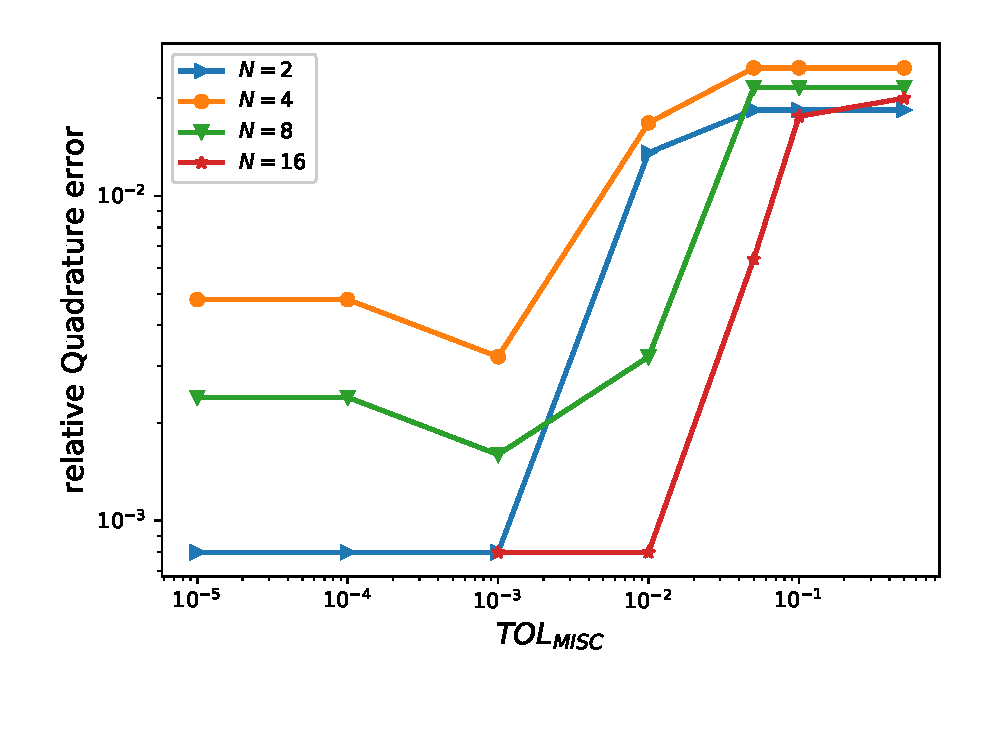
\includegraphics[width=0.4\linewidth]{./figures/rBergomi_MISC_quadratre_error/vs_TOL/set5/relative_quad_error_wrt_MISC_TOL_set5_with_rich}
	
	
	\caption{Quadrature error of MISC, with  different tolerances,  to compute call option price, for different number of time steps. Case  set $3$ parameters, with Richardson extrapolation.  See detailed values  in table \ref{Quadrature error of MISC to compute Call option price of the different tolerances for different number of time steps. Case set $3$ parameters, with Richardson extrapolation(level $1$). The numbers between parentheses are the corresponding absolute errors.}.}
	\label{fig:Quadrature_error_set3_rich}
\end{figure}
\FloatBarrier
\begin{table}[h!]
	\centering
	\begin{tabular}{l*{6}{c}r}
		Method \textbackslash  Steps           & $2-4$ & $4-8$ & $8-16$  \\
		\hline
%		MISC ($TOL_{\text{MISC}}=5.10^{-1}$)  & $0.0273$  & $0.0225$ & $0.0205$  \\
		MISC ($TOL_{\text{MISC}}=10^{-1}$)  &$0.0273$  &$0.0225$ & $0.0181$  \\
%		MISC ($TOL_{\text{MISC}}=5.10^{-2}$)  & $0.0273$  &$0.0225$ & $0.0069$  \\
			MISC ($TOL_{\text{MISC}}=10^{-2}$)  & $0.0193$  & $0.0041$ & $\red{0.0013}$  \\
		MISC ($TOL_{\text{MISC}}=10^{-3}$)  & $\red{0.0057}$  & $\red{0.0025}$ & $0.0013$  \\
%		MISC ($TOL_{\text{MISC}}=10^{-4}$)    &$0.0057$  & $0.0033$  & $-$  \\
%			MISC ($TOL_{\text{MISC}}=10^{-5}$)    &$0.0057$   &  $0.0033$ & $-$  \\	
	\hline

		MC    & $\red{\mathbf{0.0073}}$  &   $\red{\mathbf{0.0025}}$  &  $\red{\mathbf{0.0013}}$  \\
		\hline
	\end{tabular}
	\caption{Total relative error of MISC, with different tolerances, and MC to compute call option price  for different number of time steps. Case set $3$ parameters in table \ref{table:Reference solution, using MC with $500$ time steps, of Call option price under rBergomi model, for different parameter constellation.}, with Richardson extrapolation(level $1$). The numbers between parentheses are the corresponding absolute errors. The values marked in red, for MISC method, correspond to the total relative errors associated with  stable quadrature errors for MISC, and will be used for complexity comparison against MC.}
	\label{Total  error of MISC and MC to compute Call option price of the different tolerances for different number of time steps. Case set $3$ parameters, with Richardson extrapolation(level $1$). The numbers between parentheses are the corresponding absolute errors.}
\end{table}

\FloatBarrier

\begin{table}[h!]
	\centering
	\begin{tabular}{l*{6}{c}r}
		Method \textbackslash  Steps            & $2-4$ & $4-8$ & $8-16$ &   \\
		\hline
%		MISC ($TOL_{\text{MISC}}=5.10^{-1}$)    & $0.15$ & $0.25$ & $0.5$  \\
		MISC ($TOL_{\text{MISC}}=10^{-1}$)   & $0.15$ & $0.25$ & $1$  \\
%		MISC ($TOL_{\text{MISC}}=5.10^{-2}$)    &  $0.15$ & $0.25$ & $12.5$  \\
		MISC ($TOL_{\text{MISC}}=10^{-2}$)   & $0.6$ & $10$ & $\red{112}$  \\
		MISC ($TOL_{\text{MISC}}=10^{-3}$)  & $\red{3.5}$ & $\red{34}$ & $3150$ \\
%		MISC ($TOL_{\text{MISC}}=10^{-4}$) & $11$ & $328$ & $-$  \\
%		MISC ($TOL_{\text{MISC}}=10^{-5}$)   & $39$ & $2160$ & $-$  \\
		\hline	
			MC  & $\red{45}$  & $\red{438}$  & $\red{2240}$ \\
			
			\hline
				Ratio of $\left(\text{MC}/ \text{MISC} \right)$   & $\red{13}$  & $\red{13}$  & $\red{20}$ \\

		\hline
	\end{tabular}
	\caption{Comparison of the computational time (in Seconds) of  MC and MISC, using Richardson extrapolation (level $1$), used to compute call option price of the rBergomi model for different number of time steps. Case set $3$ parameters in table \ref{table:Reference solution, using MC with $500$ time steps, of Call option price under rBergomi model, for different parameter constellation.}. The
average MC CPU time is computed over 10 runs.}
	\label{Comparsion of the computational time of  MC and MISC, using Richardson extrapolation (level $1$), used to compute Call option price of rBergomi model for different number of time steps. Case set $3$ parameters}
\end{table}

\FloatBarrier


	\begin{figure}[h!]
	\centering
	\includegraphics[width=0.4\linewidth]{./figures/rBergomi_Complexity_rates/set5/error_vs_time_set5_comparison}
	
	\caption{Complexity plot for  MISC (with and without) Richardson extrapolation for case set $3$ parameters of table \ref{table:Reference solution, using MC with $500$ time steps, of Call option price under rBergomi model, for different parameter constellation.}.}
	\label{fig:Complexity plot for  MISC for case set $3$ parameters, comparison}
\end{figure}


\FloatBarrier
\subsubsection{Case of set $4$ parameters in table \ref{table:Reference solution, using MC with $500$ time steps, of Call option price under rBergomi model, for different parameter constellation.}}\label{sec:Case of set 4 parameters}
\FloatBarrier
\begin{table}[h!]
	\centering
	\begin{tabular}{l*{6}{c}r}
		Method \textbackslash  Steps            & $2$ & $4$ & $8$ & $16$ &   \\
		\hline
%		MISC ($TOL_{\text{MISC}}=5.10^{-1}$)  & $0.2413$ & $0.2403$ & $0.2403$ & $0.2396$  \\
		MISC ($TOL_{\text{MISC}}=10^{-1}$)  & $0.2413$ &$0.2403$& $0.2403$ & $0.2397$   \\
%		MISC ($TOL_{\text{MISC}}=5.10^{-2}$)  &$0.2413$ & $0.2403$ & $0.2403$ & $0.2406$  \\
		MISC ($TOL_{\text{MISC}}=10^{-2}$)  &$0.2413$ & $0.2403$ & $0.2409$ & $0.2413$  \\
		
		MISC ($TOL_{\text{MISC}}=10^{-3}$)  & $0.2413$ & $0.2411$ & $0.2414$ & $0.2413$  \\
		MISC ($TOL_{\text{MISC}}=10^{-4}$)  &  $0.2421$ & $0.2416$ & $0.2414$ & $-$  \\
		
%		MISC ($TOL_{\text{MISC}}=10^{-5}$)  & $0.2421$ &$0.2416$ &  $0.2414$ & $-$  \\
		\hline
		MC method ($M=5.10^{6}$)   & $0.2420$ & $0.2416$  & $0.2414$ & $0.2413$ \\		
		
		\hline
	\end{tabular}
	\caption{ Call option price of the different methods for different number of time steps. Case set $4$ parameters in table \ref{table:Reference solution, using MC with $500$ time steps, of Call option price under rBergomi model, for different parameter constellation.}, without Richardson extrapolation.}
	\label{table: Call option price of the different methods for different number of time steps. Case set 4}
\end{table}
\FloatBarrier

\begin{table}[h!]
	\centering
	\begin{tabular}{l*{6}{c}r}
		Method \textbackslash  Steps            & $2$ & $4$ & $8$ & $16$  \\
		\hline
		MC Bias ($M=5.10^6$)   & 	$ \underset{(    0.0013)}{\mathbf{0.0054}}$  & $\underset{(0.0008)}{\mathbf{0.0035
		}}$  & $\underset{(0.0007)}{\mathbf{0.0029}}$ & $\underset{(0.0006)}{\mathbf{0.0024}}$\\ 
		
		MC Statistical error ($M=5.10^6$)  &  $\underset{(   8.3e-05)} {\mathbf{3.4e-04}}$  & $\underset{(8.1e-05)} {\mathbf{3.4e-04}}$  & $\underset{(8.0e-05)} {\mathbf{3.3e-04 }}$ & $\underset{(8.0e-05)} {\mathbf{3.3e-04}}$	\\
		
		\hline
	\end{tabular}
	\caption{Bias and statistical errors of MC   for computing call option price  for different number of time steps. Case set $4$, without Richardson extrapolation. The numbers between parentheses are the corresponding absolute errors.}
	\label{Bias and Statistical errors of MC ($M=5.10^6$)  for computing Call option price  for different number of time steps. Case set 4, without Richardson extrapolation. The numbers between parentheses are the corresponding absolute errors.}
\end{table}


\FloatBarrier


\begin{figure}[h!]
	\centering
	\includegraphics[width=0.4\linewidth]{./figures/rBergomi_MISC_quadratre_error/vs_TOL/set6/relative_quad_error_wrt_MISC_TOL_set6_non_rich}
	
	
	\caption{Quadrature error of MISC, with different tolerances, to compute call option price  for different number of time steps. Case  set $4$ parameters, without Richardson extrapolation.  See detailed values  in table \ref{Quadrature error of MISC to compute Call option price of the different tolerances for different number of time steps. Case  set $4$ parameters, without Richardson extrapolation. The numbers between parentheses are the corresponding absolute errors.}}
	\label{fig:Quadrature_error_set4}
\end{figure}



\FloatBarrier

\begin{table}[h!]
	\centering
	\begin{tabular}{l*{6}{c}r}
		Method \textbackslash  Steps            & $2$ & $4$ & $8$ & $16$  \\
		\hline
%		MISC ($TOL_{\text{MISC}}=5.10^{-1}$)  & $\mathbf{0.0083}$ & $\mathbf{0.0089}$ & $\mathbf{ 0.0075}$ & $\mathbf{ 0.0095}$  \\
		MISC ($TOL_{\text{MISC}}=10^{-1}$)  &  $\mathbf{0.0083}$ & $\mathbf{0.0089}$& $\mathbf{ 0.0075}$ & $\mathbf{ 0.0090}$   \\
%		MISC ($TOL_{\text{MISC}}=5.10^{-2}$)  & $\mathbf{0.0083}$ & $\mathbf{0.0089}$ & $\mathbf{ 0.0075}$ & $\mathbf{ 0.0057}$  \\
		MISC ($TOL_{\text{MISC}}=10^{-2}$)  &  $\mathbf{0.0083}$ & $\mathbf{0.0089}$& $\mathbf{ 0.0050}$ & $\mathbf{ \red{0.0025}}$  \\
		MISC ($TOL_{\text{MISC}}=10^{-3}$)  &  $\mathbf{0.0083}$& $\mathbf{0.0056}$& $\mathbf{\red{0.0030}}$  & $\mathbf{ 0.0025}$  \\
		MISC ($TOL_{\text{MISC}}=10^{-4}$)  &  $\mathbf{\red{0.0058}}$ & $\mathbf{\red{0.0037}}$& $\mathbf{0.0030}$ & $\mathbf{ -}$ \\
%		MISC ($TOL_{\text{MISC}}=10^{-5}$)  &  $\mathbf{0.0058}$ & $\mathbf{0.0037}$& $\mathbf{0.0030}$ & $\mathbf{ -}$ 
		
		\hline
		MC    & $\mathbf{\red{0.0057}}$  & $\mathbf{ \red{0.0038}}$  & $\mathbf{\red{0.0032}}$ & $\mathbf{ \red{0.0027}}$  \\		
		\hline
	\end{tabular}
	\caption{Total relative error of MISC,different tolerances, and MC to compute call option price  for different number of time steps. Case set $4$ parametrs of table \ref{table:Reference solution, using MC with $500$ time steps, of Call option price under rBergomi model, for different parameter constellation.}, without Richardson extrapolation. The numbers between parentheses are the corresponding absolute errors. The values marked in red, for MISC method, correspond to the total relative errors associated with  stable quadrature errors for MISC, and will be used for complexity comparison against MC.}
	\label{Total error of MISC and MC to compute Call option price of the different tolerances for different number of time steps. Case set 4, without Richardson extrapolation. The numbers between parentheses are the corresponding absolute errors.}
\end{table}

\FloatBarrier
\begin{table}[h!]
	\centering
	\begin{tabular}{l*{6}{c}r}
		Method \textbackslash  Steps            & $2$ & $4$ & $8$ & $16$ &   \\
		\hline
%		MISC ($TOL_{\text{MISC}}=5.10^{-1}$)  & $0.1$ & $0.1$ & $0.1$ & $0.3$  \\
		MISC ($TOL_{\text{MISC}}=10^{-1}$)  & $0.1$ & $0.1$ & $0.1$ & $1$ \\
%		MISC ($TOL_{\text{MISC}}=5.10^{-2}$)  & $0.1$ & $0.1$ & $0.1$ & $22$  \\
		MISC ($TOL_{\text{MISC}}=10^{-2}$)  & $0.1$ & $0.15$ & $9$ & $\red{112}$ \\
		MISC ($TOL_{\text{MISC}}=10^{-3}$)  & $0.2$ & $2$ & $\red{27}$ & $2226$ \\
		MISC ($TOL_{\text{MISC}}=10^{-4}$)  & $\red{1}$ & $\red{6}$ & $136$ & $-$\\
%		MISC ($TOL_{\text{MISC}}=10^{-5}$)  & $2$ & $18$ & $1559$ & $-$
%		\\
		\hline
		MC method   & $ \red{141}
		
		$  & $  \red{246}$  & $  \red{461}$ & $ \red{820}
		$  \\	
		\hline
		Ratio of $\left(MC/MISC \right)$ & $ \red{141}
		
		$  & $  \red{
			41
		}$  & $  \red{    17
		}$ & $ \red{ 7}
		$  \\	
%		
		\hline
	\end{tabular}
	\caption{Comparison of the computational time (in Seconds) of  MC and MISC, used to compute call option price of the rBergomi model for different number of time steps. Case set $4$ parameters of table \ref{table:Reference solution, using MC with $500$ time steps, of Call option price under rBergomi model, for different parameter constellation.}. The average  MC CPU time is computed over $10$ runs. }
	\label{Comparsion of the computational time of  MC and MISC, used to compute Call option price of rBergomi model for different number of time steps. Case set4}
\end{table}


\FloatBarrier

	\begin{figure}[h!]
	\centering
	\includegraphics[width=0.4\linewidth]{./figures/rBergomi_Complexity_rates/set6/error_vs_time_set6}
	
	\caption{Complexity plot for   MC and MISC for case set $4$ parameters of table \ref{table:Reference solution, using MC with $500$ time steps, of Call option price under rBergomi model, for different parameter constellation.}.}
	\label{fig:Complexity plot for MC and MISC for case set $4$ parameters}
\end{figure}
\FloatBarrier
\subsubsection{Case of set $5$ parameters in table \ref{table:Reference solution, using MC with $500$ time steps, of Call option price under rBergomi model, for different parameter constellation.}}\label{sec:Case of set 5 parameters}
\FloatBarrier
\begin{table}[h!]
	\centering
	\begin{tabular}{l*{6}{c}r}
		Method \textbackslash  Steps            & $2$ & $4$ & $8$ & $16$ &   \\
		\hline
%		MISC ($TOL_{\text{MISC}}=5.10^{-1}$)  & $0.0590$ & $0.0564$ & $0.0552$ & $0.0546$  \\
		MISC ($TOL_{\text{MISC}}=10^{-1}$)  & $0.0590$ &$0.0564$& $0.0552$ & $0.0546$   \\
%		MISC ($TOL_{\text{MISC}}=5.10^{-2}$)  &$0.0590$ & $0.0564$ & $0.0552$ & $0.0557$  \\
		MISC ($TOL_{\text{MISC}}=10^{-2}$)  &$0.0590$ &$0.0564$ & $0.0574$ & $0.0572$  \\
		
		MISC ($TOL_{\text{MISC}}=10^{-3}$)  & $0.0605$ & $0.0587$ & $0.0579$ & $0.0575$  \\
%		MISC ($TOL_{\text{MISC}}=10^{-4}$)  &  $0.0605$ & $0.0587$ & $0.0576$ & $-$  \\
%		
%		MISC ($TOL_{\text{MISC}}=10^{-5}$)  & $0.0605$ & $0.0587$ &  $0.0579$ & $-$  \\
		\hline
		MC method ($M=5.10^{6}$)   & $0.0605$ & $0.0587$  & $0.0579$ & $0.0576$ \\		
		
		\hline
	\end{tabular}
	\caption{ Call option price of the different methods for different number of time steps. Case of set $5$ parameters in table \ref{table:Reference solution, using MC with $500$ time steps, of Call option price under rBergomi model, for different parameter constellation.}, without Richardson extrapolation.}
	\label{table: Call option price of the different methods for different number of time steps. Case set 5}
\end{table}

\FloatBarrier
\begin{table}[h!]
	\centering
	\begin{tabular}{l*{6}{c}r}
		Method \textbackslash  Steps            & $2$ & $4$ & $8$ & $16$  \\
		\hline
		MC Bias ($M=5.10^6$)   & 	$ \underset{(0.0037
			)}{\mathbf{0.0650}}$  & $\underset{(0.0019)}{\mathbf{0.0330
		}}$  & $\underset{(0.0012)}{\mathbf{0.0202}}$ & $\underset{(0.0007)}{\mathbf{0.0130}}$\\ 
		
		MC Statistical error ($M=5.10^6$)  &  $\underset{(   4.0e-05)} {\mathbf{7.0e-04}}$  & $\underset{(3.8e-05)} {\mathbf{6.7e-04}}$  & $\underset{(3.7e-05)} {\mathbf{6.5e-04 }}$ & $\underset{(3.6e-05)} {\mathbf{6.3e-04}}$	\\
		
		\hline
	\end{tabular}
	\caption{Bias and statistical errors of MC   for computing call option price  for different number of time steps. Case set $5$, without Richardson extrapolation. The numbers between parentheses are the corresponding absolute errors.}
	\label{Bias and Statistical errors of MC ($M=5.10^6$)  for computing Call option price  for different number of time steps. Case set 5, without Richardson extrapolation. The numbers between parentheses are the corresponding absolute errors.}
\end{table}
%
%
%


\FloatBarrier





\begin{figure}[h!]
	\centering
	\includegraphics[width=0.4\linewidth]{./figures/rBergomi_MISC_quadratre_error/vs_TOL/set7/relative_quad_error_wrt_MISC_TOL_set7_non_rich}
	
	
	\caption{Quadrature error of MISC, with  different tolerances,  to compute call option price  for different number of time steps. Case  set $5$ parameters, without Richardson extrapolation.  See detailed values  in table \ref{Quadrature error of MISC to compute Call option price of the different tolerances for different number of time steps. Case  set $5$ parameters, without Richardson extrapolation. The numbers between parentheses are the corresponding absolute errors.}}
	\label{fig:Quadrature_error_set5}
\end{figure}

\FloatBarrier
%
%
%
\begin{table}[h!]
	\centering
	\begin{tabular}{l*{6}{c}r}
		Method \textbackslash  Steps            & $2$ & $4$ & $8$ & $16$  \\
		\hline
%		MISC ($TOL_{\text{MISC}}=5.10^{-1}$)  & $\mathbf{0.0914}$ & $\mathbf{0.0736}$ & $\mathbf{ 0.0693}$ & $\mathbf{ 0.0654}$  \\
		MISC ($TOL_{\text{MISC}}=10^{-1}$)  & $\mathbf{0.0914}$ & $\mathbf{0.0736}$& $\mathbf{ 0.0693}$ & $\mathbf{ 0.0654}$   \\
%		MISC ($TOL_{\text{MISC}}=5.10^{-2}$)  & $\mathbf{0.0914}$ & $\mathbf{0.0736}$ & $\mathbf{ 0.0693}$ & $\mathbf{ 0.0461}$  \\
		MISC ($TOL_{\text{MISC}}=10^{-2}$)  &  $\mathbf{0.0914}$& $\mathbf{0.0736}$& $\mathbf{ 0.0223}$ & $\mathbf{ 0.0195}$  \\
		MISC ($TOL_{\text{MISC}}=10^{-3}$)  &  $\mathbf{\red{0.0655}}$& $\mathbf{\red{0.0334}}$& $\mathbf{\red{0.0205}}$  & $\mathbf{ \red{0.0135}}$  \\
%		MISC ($TOL_{\text{MISC}}=10^{-4}$)  &  $\mathbf{0.0655}$& $\mathbf{0.0334}$& $\mathbf{0.0205}$ & $\mathbf{ -}$ \\
%		MISC ($TOL_{\text{MISC}}=10^{-5}$)  &  $\mathbf{0.0655}$ & $\mathbf{0.0334}$& $\mathbf{0.0205}$ & $\mathbf{ -}$ 
%		\\
		\hline
		MC    & $\mathbf{\red{0.0657}}$  & $\mathbf{ \red{0.0337}}$  & $\mathbf{\red{0.0209}}$ & $\mathbf{ \red{0.0136}}$  \\		
		\hline
	\end{tabular}
	\caption{Total relative error of MISC, with  different tolerances,  and MC to compute call option price  for different number of time steps. Case  set $5$ parametrs of table \ref{table:Reference solution, using MC with $500$ time steps, of Call option price under rBergomi model, for different parameter constellation.}, without Richardson extrapolation. The numbers between parentheses are the corresponding absolute errors. The values marked in red, for MISC method, correspond to the total relative errors associated with  stable quadrature errors for MISC, and will be used for complexity comparison against MC.}
	\label{Total error of MISC and MC to compute Call option price of the different tolerances for different number of time steps. Case set 5, without Richardson extrapolation. The numbers between parentheses are the corresponding absolute errors.}
\end{table}

\FloatBarrier
\begin{table}[h!]
	\centering
	\begin{tabular}{l*{6}{c}r}
		Method \textbackslash  Steps            & $2$ & $4$ & $8$ & $16$ &   \\
		\hline
%		MISC ($TOL_{\text{MISC}}=5.10^{-1}$)  & $0.1$ & $0.1$ & $0.2$ & $0.5$  \\
		MISC ($TOL_{\text{MISC}}=10^{-1}$)  & $0.1$ & $0.1$ & $0.2$ & $0.5$ \\
%		MISC ($TOL_{\text{MISC}}=5.10^{-2}$)  & $0.1$ & $0.1$ & $0.2$ & $5$  \\
		MISC ($TOL_{\text{MISC}}=10^{-2}$)  & $0.1$ & $0.1$ & $8$ & $97$ \\
		MISC ($TOL_{\text{MISC}}=10^{-3}$)  & $\red{0.7}$ & $\red{4}$ & $\red{26}$ & $\red{1984}$ \\
%		MISC ($TOL_{\text{MISC}}=10^{-4}$)  & $1$ & $8$ & $173$ & $-$\\
%		MISC ($TOL_{\text{MISC}}=10^{-5}$)  & $1$ & $32$ & $2129$ & $-$
%		\\
		\hline
		MC method   & $ \red{154}
		
		$  & $  \red{229}$  & $  \red{420}$ & $ \red{938}
		$  \\	
		\hline
		Ratio of $\left(MC/MISC \right)$ & $ \red{   220}
		
		$  & $  \red{
		 57
		}$  & $  \red{    16
		}$ & $ \red{ 0.5}
		$  \\	
				
		\hline
	\end{tabular}
	\caption{Comparison of the computational time (In seconds) of  MC and MISC, used to compute call option price of rBergomi model for different number of time steps. Case set $5$ parametrs of table \ref{table:Reference solution, using MC with $500$ time steps, of Call option price under rBergomi model, for different parameter constellation.}. The average  MC CPU time is computed over $10$ runs. }
	\label{Comparsion of the computational time of  MC and MISC, used to compute Call option price of rBergomi model for different number of time steps. Case set5}
\end{table}

\FloatBarrier


	\begin{figure}[h!]
	\centering
	\includegraphics[width=0.4\linewidth]{./figures/rBergomi_Complexity_rates/set7/error_vs_time_set7}
	
	\caption{Complexity plot for   MC and MISC for case set $5$ parameters of table \ref{table:Reference solution, using MC with $500$ time steps, of Call option price under rBergomi model, for different parameter constellation.}.}
	\label{fig:Complexity plot for MC and MISC for Case set $5$ parameters}
\end{figure}
\FloatBarrier







\section{Conclusions and future work}

In this work,  we propose  novel, fast option pricers,  for options whose underlyings  follow the rBergomi model as in \cite{bayer2016pricing}.  The new methods  are based on hierarchical deterministic quadrature methods:  i) ASGQ using the same construction as in \cite{haji2016multi}, and ii) the QMC method. Both techniques are coupled with Brownian bridge construction and Richardson extrapolation.

Given that the only prevalent option, in this context, is to use different variants of the MC method, which is computationally expensive, our first contribution  is that we uncover the available regularity in the rBergomi model and  design novel  approaches based on an ASGQ and QMC. These approaches  open a new research direction in this field to investigate the performance of other methods besides MC, for pricing and calibrating under the rBergomi model. Our second contribution is that we reduce the computational cost  through bias reduction by using Richardson extrapolation. Finally, assuming one targets price estimates with a sufficiently small relative error tolerance, our proposed method demonstrates substantial computational gains  over the standard MC method, when pricing under the rBergomi model, even for very small values of the Hurst parameter. We show  these gains through our numerical experiments for  different parameter constellations.  We clarify that we do not claim that these gains will hold in the asymptotic regime, i.e.,  for higher accuracy requirements. Furthermore, the use of Richardson extrapolation is justified in the pre-asymptotic regime, in which our observed experimental results suggest a convergence of order one for the weak error. We emphasize that, to the best of our knowledge, no proper weak error analysis has been done in the rough volatility context. 

In this work, we limit ourselves to compare our novel proposed method against the standard MC. A more systematic comparison against the variant of MC proposed in \cite{mccrickerd2018turbocharging}  can be carried out but this remains for a future study. Another future research direction is to provide a reliable method for controlling the quadrature error for ASGQ which is,  to the best of our knowledge,  still  an open research problem. This is even more challenging in our context, especially for low values of $H$. We emphasize that the main aim of this work is to illustrate the high potential of deterministic quadrature, when coupled with hierarchical representations, for pricing options under the rBergomi model.   Finally, accelerating  our novel  methods can be achieved  by using better versions of the ASGQ or QMC methods.


\

\textbf{Acknowledgments} C. Bayer gratefully acknowledges support from the German Research Foundation (DFG, grant BA5484/1). This work was supported by the KAUST Office of Sponsored Research (OSR) under Award No. URF/1/2584-01-01 and the Alexander von Humboldt Foundation. C. Ben Hammouda and R. Tempone are members of the KAUST SRI Center for Uncertainty Quantification in Computational Science and Engineering. The authors would like to thank Joakim Beck, Eric Joseph Hall and Erik von Schwerin for their helpful and constructive comments that greatly contributed to improving the final version of the paper. 



 %%%%%%%%%%%%%%%%%%%%%%%%%%%%%%%%%%%%%%%%%%
%References
%%%%%%%%%%%%%%%%%%%%%%%%%%%%%%%%%%%%%%%%%%

\bibliographystyle{plain}
\bibliography{smoothing_rBergomi.bib} 




%\appendix
%%\section{ Prices for different methods for binary option }\label{appendix:Call prices for different methods_binary}
%
%\begin{table}[h!]
%	\centering
%	\begin{tabular}{l*{6}{c}r}
%		Method \textbackslash  Steps            & $2$ & $4$ & $8$ & $16$ &   \\
%		\hline
%		MISC ($TOl=5.10^{-1}$)  & $\red{0.4619}$ & $  \red{0.4404}$ & $\red{0.4299}$ & $\red{0.4250}$  \\
%		\hline
%	\end{tabular}
%	\caption{ Binary option price of the different methods for different number of time steps, without Richardson extrapolation.}
%	\label{table: Binary option price of the different methods for different number of time steps}
%\end{table}
%
%
%\begin{table}[h!]
%	\centering
%	\begin{tabular}{l*{6}{c}r}
%		Method \textbackslash  Steps   &$1-2$         & $2-4$ & $4-8$ & $8-16$  \\
%		\hline
%		MISC ($TOl=5.10^{-1}$) & $\red{0.4239}$ & $0.4188$ & $  0.4194$ & $0.4200$   \\
%			MISC ($TOl=10^{-2}$) & $-$ & $\red{0.4192}$ & $  0.4194$ & $0.4201$   \\
%			MISC ($TOl=10^{-3}$) & $-$ & $-$ & $  \red{0.4198}$ & $\red{0.4205}$   \\
%		\hline
%	\end{tabular}
%	\caption{Binary  option price of the different methods for different number of time steps, with Richardson extrapolation (level $1$).}
%	\label{table: Binary option price of the different methods for different number of time steps, binary option, with richardson, level 1}
%\end{table}
%
%\newpage
%
%
%\section{ Call prices for different methods}\label{appendix:Call prices for different methods}
%
%\begin{table}[h!]
%	\centering
%	\begin{tabular}{l*{6}{c}r}
%		Method \textbackslash  Steps            & $2$ & $4$ & $8$ & $16$ &   \\
%		\hline
%		MISC ($TOl=5.10^{-1}$)  & $\red{16.2145}$ & $16.1352$ & $\red{16.0275}$ & $\red{15.9594}$  \\
%			MISC ($TOl=10^{-3}$)  & $-$ & $ \red{16.1328 }$ & $-$ & $-$  \\
%		\hline
%	\end{tabular}
%	\caption{ Call option price of the different methods for different number of time steps, without Richardson extrapolation.}
%	\label{table: Call option price of the different methods for different number of time steps}
%\end{table}
%
%
%\begin{table}[h!]
%	\centering
%	\begin{tabular}{l*{6}{c}r}
%		Method \textbackslash  Steps   &$1-2$         & $2-4$ & $4-8$ & $8-16$  \\
%		\hline
%		MISC ($TOl=5.10^{-1}$) & $\red{16.4419}$ & $16.0558$ & $15.9205$ & $15.8915$   \\
%		MISC ($TOl=10^{-3}$) & $-$ & $\red{16.0510}$ & $ \red{15.9177}$ & $\red{15.8880}$   \\
%		\hline
%	\end{tabular}
%	\caption{Call  option price of the different methods for different number of time steps, with Richardson extrapolation (level $1$).}
%	\label{table: Call option price of the different methods for different number of time steps, binary option, with richardson, level 1}
%\end{table}
%
%\begin{table}[h!]
%	\centering
%	\begin{tabular}{l*{6}{c}r}
%		Method \textbackslash  Steps   &$1-2-4$         & $2-4-8$ & $4-8-16$   \\
%		\hline
%		MISC ($TOl=5.10^{-1}$) & $15.9269$ & $15.8756$ & $15.8815$  \\
%		MISC ($TOl=10^{-3}$) & $\red{15.9205}$ & $\red{15.8732}$ & $ \red{  15.8789}$   \\
%		\hline
%	\end{tabular}
%	\caption{Call option price of the different methods for different number of time steps, with Richardson extrapolation (level $2$).}
%	\label{table: Call option price of the different methods for different number of time steps, binary option, with richardson, level 2}
%\end{table}
%\newpage



%
%\section{Results of the basket example}
%\subsubsection{Verifying bounds on work and error contributions}
%
%In this subsection, we discuss the validity of Assumptions $2$-$4$ in \cite{haji2016multi}, upon which the MISC convergence theorem is based. In this case, basket option case we do not use a deterministic solver since the we have a close for of the integrand and then  we analyze  only the properties of the collocation method applied to
%the problem.
%
%
%
%
%Below, we show in figures (\ref{fig:test_basket_1},\ref{fig:test_basket_2},\ref{fig:test_basket_3}) the rate of convergence of first and mixed differences for different orders and we check that the error is decaying exponentially wrt number of points used in the quadrature.
%
%	
%	\begin{figure}[h!]
%		\centering
%		\begin{subfigure}{.5\textwidth}
%			\centering
%			\includegraphics[width=1\linewidth]{./figures/first_difference_basket.eps}
%			\caption{}
%			\label{fig:sub1}
%		\end{subfigure}%
%		\begin{subfigure}{.5\textwidth}
%			\centering
%			\includegraphics[width=1\linewidth]{./figures/mixed_difference_order2_basket_1.eps}
%			\caption{}
%			\label{fig:sub2}
%		\end{subfigure}%
%		\caption{The rate of convergence of $\abs{\Delta E_{\beta}}$ ($\beta=\mathbf{1}+k \bar{\beta}$): a) shows the rate of convergence of first order differences. b)  shows the rate of convergence of second order mixed differences.}
%			\label{fig:test_basket_1}
%	\end{figure}
%
%	\begin{figure}
%	\centering
%	\begin{subfigure}{.5\textwidth}
%		\centering
%		\includegraphics[width=1\linewidth]{./figures/mixed_difference_order2_basket_2.eps}
%		\caption{}
%		\label{fig:sub3}
%	\end{subfigure}%
%	\begin{subfigure}{.5\textwidth}
%		\centering
%		\includegraphics[width=1\linewidth]{./figures/mixed_difference_order2_basket_3.eps}
%		\caption{}
%		\label{fig:sub4}
%	\end{subfigure}
%
%	\caption{The rate of convergence of $\abs{\Delta E_{\beta}}$ ($\beta=\mathbf{1}+k \bar{\beta}$)): a) and b) show  the rate of convergence of second order mixed differences for different settings.}
%		\label{fig:test_basket_2}
%\end{figure}
%
%	\begin{figure}
%	\centering
%	\begin{subfigure}{.5\textwidth}
%		\centering
%		\includegraphics[width=1\linewidth]{./figures/mixed_difference_order3_basket_1.eps}
%	    \caption{}
%		\label{fig:sub5}
%	\end{subfigure}%
%	\begin{subfigure}{.5\textwidth}
%		\centering
%		\includegraphics[width=1\linewidth]{./figures/mixed_difference_order3_basket_2.eps}
%		\caption{}
%		\label{fig:sub6}
%	\end{subfigure}
%	
%	\caption{The rate of convergence of $\abs{\Delta E_{\beta}}$ ($\beta=\mathbf{1}+k \bar{\beta}$): a) and b) show  the rate of convergence of third order mixed differences for different settings.}
%	\label{fig:test_basket_3}
%\end{figure}
%
%
%
% \newpage
%\section{Implementation details and  MISC results}\label{sec:Implementation details and  MISC results}
%The first step, when testing this example is to fix $\Delta t_{\text{min}}$ for the  time discretization parameter and do not introduce a hierarchy of levels in the deterministic dimension. Therefore, we will only construct a hierarchy of levels in the stochastic dimension associated with the Brownian increments. Then, the second step is to avoid this restriction of minimum  time discretization parameter (somehow like letting $\Delta t_{\text{min}} \rightarrow 0$)  and in that case, the problem will be close to do the integration in $\infty$-dimension, we need to see how the convergence rates will behave. The third step, is to use Richardson extrapolation which we expect bring the order of convergence for the Euler scheme from $ \ordo{\Delta t}$  to  $\ordo{\Delta t^2}$, and then we may expect that we will need fewer time steps to converge than the first case, and which means that fewer stochastic directions will be activated.   One technical difference here is that for $1$-dimensional, we will have two kink points instead of one but the procedure will be the same.  We note that we used Laguerre quadrature for integrating with respect to the dimension containing the kink. 
%
%Since we observed some problems for the results of the non-smooth payoff with Richardson extrapolation, we tried to add another case where we use a smoothed version of the call payoff to figure out the source of the problem. Using a smooth payoff allow us to separate the effect of infinite dimension and non-smoothness. As a possible choice, we use  the Black Scholes call option price formula, given by 
%\begin{equation}
%\mathrm C(\mathrm S,\mathrm t)= \mathrm N(\mathrm d_1)\mathrm S - \mathrm N(\mathrm d_2) \mathrm K \mathrm e^{-rt}
%\label{eq:2}
%\end{equation}
%
%\begin{equation}
%\mathrm d_1= \frac{1}{\sigma \sqrt{\mathrm t}} \left[\ln{\left(\frac{S}{K}\right)} + t\left(r + \frac{\sigma^2}{2} \right) \right]
%\end{equation}
%
%\begin{equation}
%\mathrm d_2= d_1- \sigma  \sqrt{t} 
%\end{equation}
%
%\begin{equation}
%N(x)=\frac{1}{\sqrt{2\pi}} \int_{-\infty}^{x} \mathrm e^{-\frac{1}{2}z^2} dz
%\label{eq:5}
%\end{equation}
%
%
%, which can be seen as a smoothed version of the true payoff (See figure \ref{fig:smooth_non_smooth}). The two differences with respect to the non-smooth case is that the dimension of the parameter space (stochastic space) now is increased by one  due to including the terminal value of the driving Brownian motion. Numerically, we observed weird results , in fact the quadrature performed worse than with the non-smooth case,  even for various values of volatilities. We still need to understand why this choice is not a good one. 
%
%
%Another possible choice that we worked with,  is by using the following smooth approximation of the max call payoff (See figure \ref{fig:smooth_payoff2})
%
%\begin{align}\label{eq:smooth_payoff2}
%	\operatorname{\max}_\epsilon(S-K,0) \approx 0.5 ( S-K+\sqrt{ (S-K)^{2}+\epsilon}),
%\end{align}
%
%where $\epsilon>0$.
%
%
%
%
%
%
%
%\begin{figure}[!h]
%	\centering
%	\begin{subfigure}{.5\textwidth}
%		\centering
%		\includegraphics[width=1\linewidth]{./figures/smooth_non_smooth_payoff.png}
%		\caption{Black Scholes call option price for different values of $\sigma$}
%		\label{fig:smooth_non_smooth}
%	\end{subfigure}%
%	\begin{subfigure}{.5\textwidth}
%		\centering
%		\includegraphics[width=1\linewidth]{./figures/smooth_payoff_2.png}
%		\caption{Smooth approximation of the max call payoff for different values of $\epsilon$.}
%		\label{fig:smooth_payoff2}
%	\end{subfigure}%
%\end{figure}
%
%
%
%%Numerically, we tried different values of $\epsilon$. For values of $\epsilon<10^5$, it is much expensive to run the quadrature compared to the non-smooth case( we need to understand why we have this behavior). 
%%In section \ref{sec:Results using MISC code_1D_BS}, we show some of the results with $8$ time steps and for $\epsilon=10^5$.
%%
%%\newpage
%%\subsubsection{A smooth payoff with Richardson extrapolation}
%%In this section, we present Richardson extrapolation algorithm that we use to compute the integrand before passing it to misc for the quadrature. We expect a slighter improvement of the rates  compared to cases without using Richardson extrapolation since $dt$ is fixed in the misc code (we assume that we do not have a deterministic direction, just stochastic ones). However, this improvement should be much better as $dt\rightarrow 0$ (higher number of time steps). In fact, since the convergence is fast with respect to the stochastic dimensions, the rate of convergence is deteriorated by the time-stepping procedure and then the advantage of using   Richardson extrapolation is to bring the order of convergence for the Euler scheme from $ \ordo{\Delta t}$  to  $\ordo{\Delta t^\alpha}$ ($\alpha>1$). This improvement implies that fewer stochastic directions will be activated and thus the improvement of the global rate of convergence.
%%
%%\begin{algorithm}
%%	\caption{Description of the Richardson algorithm }\label{euclid}
%%	\begin{algorithmic}[1]
%%%		\Procedure{MyProcedure}{}
%%		\State Initial set of quadrature points $y$, initial number of time steps $N$, $n:$ level of Richardson extrapolation, $\tilde{g}:$ the smooth payoff approximation
%%		\For{\texttt{$i=0$ to $n$}}
%%		\State $d_i0 \leftarrow \tilde{g}(\bar{X}_{N})$  ($\bar{X}_{N}$ is the stock price simulated with $N$ time steps and using $N$ quadrature points form $y$)
%%			\For{\texttt{$j=1$ to $i$}}
%%			\State $d_{i,j} \leftarrow d_{i,j-1}+(d_{i,j-1}-d_{i-1,j-1})/(4^j-1)$
%%			\EndFor
%%		\State $N \leftarrow 2 N	$
%%		\EndFor
%%		
%%		
%%		
%%%		\State $i \gets \textit{patlen}$
%%%		\BState \emph{top}:
%%%		\If {$i > \textit{stringlen}$} \Return false
%%%		\EndIf
%%%		\State $j \gets \textit{patlen}$
%%%		\BState \emph{loop}:
%%%		\If {$\textit{string}(i) = \textit{path}(j)$}
%%%		\State $j \gets j-1$.
%%%		\State $i \gets i-1$.
%%%		\State \textbf{goto} \emph{loop}.
%%%		\State \textbf{close};
%%%		\EndIf
%%%		\State $i \gets i+\max(\textit{delta}_1(\textit{string}(i)),\textit{delta}_2(j))$.
%%%		\State \textbf{goto} \emph{top}.
%%%		\EndProcedure
%%	\end{algorithmic}
%%\end{algorithm}
%%
%%
%%
%%
%
%
%%In the simulation, we  use consistent Brownian increments in simulating the paths of $\hat{X}^h$ and $\hat{X}^{2h}$, which results in a substantial reduction in variance. More specifically, each Brownian increment driving $\hat{X}^{2h}$ is the sum of two of the increments driving $\hat{X}^{h}$. This means that if we use $\sqrt{h} Z_1,\sqrt{h} Z_2,\dots $ as the Brownian increments for  $\hat{X}^{h}$ then we can use  $\sqrt{h} (Z_1+Z_2),\sqrt{h} (Z_3+Z_4),\dots $  as the Brownian increments for $\hat{X}^{2h}$.
%
%
%
%
%
%
%
%
%In table \ref{table: Complexity rates of the different methods for different number of time steps}, we summarize the results that we get in terms of complexity rates for different methods using different number of time steps. We clarify that the results for the Richardson extrapolation are given for just one level, where the associated steps in the table corresponds to those of level $1$.
%\begin{table}[h!]
%	\centering
%	\begin{tabular}{l*{6}{c}r}
%		Method \textbackslash  Steps            & $2$ & $4$ & $8$ & $16$  \\
%		\hline
%		Non-smooth payoff   & $-1/5$ & $-1/5$ & $-2/5$ & $-7/10$  \\
%		Non-smooth payoff with Richardson  extrapolation    & $-$ & $-$ & $-$ & $-$  \\
%		Smooth payoff(given by \eqref{eq:smooth_payoff2},$\epsilon=10^{-5}$)          & $-1/3$ &$-1/3$ &  $-3/5$ &  $-1$ \\
%		Smooth payoff with Richardson  extrapolation      & - & $-1/10$  & $-4/10$ & $-$  \\
%		\hline
%	\end{tabular}
%	\caption{Complexity rates of the different methods for different number of time steps}
%	\label{table: Complexity rates of the different methods for different number of time steps}
%\end{table}	
%
%Detailed plots for each case are given in appendix \ref{app: MISC Results 1D_BS}. Mainly, from the plots, 
%we checked  that we achive the prescribed tolerance using MISC, the convergence rates of mixed differences which is a basic assumption for using MISC (we observe exponential decay of error rates wrt to the number of quadrature points) and finally the complexity rates.
%
%\section{ MISC Results for the call option under discretized BS model}\label{app: MISC Results 1D_BS}
%
%\subsection{Case of $2$ time steps with non-smooth payoff}
%
%From the following plots, we confirm the exponential rate of convergence for the stochastic parameters, we achieve the prescribed tolerance and  we get a rate of complexity (in terms of average running time) approximately of order $-1/5$ for $2$ time steps.
%\begin{figure}[!h]
%	\centering
%	\begin{subfigure}{.5\textwidth}
%		\centering
%		\includegraphics[width=1\linewidth]{./figures/1D_BS_2_steps_non_smooth/error_estimate.pdf}
%		\caption{Error estimate}
%		\label{fig:misc_1D_BS_non_smooth_2steps_sub1}
%	\end{subfigure}%
%	\begin{subfigure}{.5\textwidth}
%		\centering
%		\includegraphics[width=1\linewidth]{./figures/1D_BS_2_steps_non_smooth/average_running_time.pdf}
%		\caption{Average running time as a function of $TOL$}
%		\label{fig:misc_1D_BS_non_smooth_2steps_sub2}
%	\end{subfigure}%
%	\caption{Convergence and complexity results for for the $1D$ BS model with the non-smooth call payoff.}
%	\label{fig:misc_1D_BS_nonsmooth_2steps_2}
%\end{figure}
%
%
%
%\begin{figure}[!h]
%	\centering
%	\begin{subfigure}{.5\textwidth}
%		\centering
%		\includegraphics[width=0.95\linewidth]{./figures/1D_BS_2_steps_non_smooth/level_work.pdf}
%		\caption{Average Computational time per level}
%		\label{fig:misc_1D_BS_non_smooth_2steps_sub3}
%	\end{subfigure}%
%	\begin{subfigure}{.5\textwidth}
%		\centering
%		\includegraphics[width=0.95\linewidth]{./figures/1D_BS_2_steps_non_smooth/levels_error_rate.pdf}
%		\caption{ The convergence rate of first differences per level}
%		\label{fig:misc_1D_BS_non_smooth_2steps_sub4}
%	\end{subfigure}%
%	\caption{Convergence and work rates for discretization levels for the $1D$ BS model with the non-smooth call payoff.}
%	\label{fig:misc_1D_BS_2teps_2}
%\end{figure}
%
%
%
%\subsection{Case of $2$ time steps with smooth payoff (given by \eqref{eq:smooth_payoff2})}
%
%From the following plots, we confirm the exponential rate of convergence for the stochastic parameters, we achieve the prescribed tolerance and  we get a rate of complexity (in terms of average running time) approximately of order $-1/3$ for $2$ time steps.
%
%\begin{figure}[!h]
%	\centering
%	\begin{subfigure}{.5\textwidth}
%		\centering
%		\includegraphics[width=1\linewidth]{./figures/1D_BS_2_steps_smooth_second_payoff_eps_10_5/error_estimate.pdf}
%		\caption{Error estimate}
%		\label{fig:misc_1D_BS_2_steps_smooth_second_payoff_eps_10_5_sub1}
%	\end{subfigure}%
%	\begin{subfigure}{.5\textwidth}
%		\centering
%		\includegraphics[width=1\linewidth]{./figures/1D_BS_2_steps_smooth_second_payoff_eps_10_5/average_running_time.pdf}
%		\caption{Average running time as a function of $TOL$}
%		\label{fig:misc_1D_BS_2_steps_smooth_second_payoff_eps_10_5_sub2}
%	\end{subfigure}%
%	\caption{Convergence and complexity results for for the $1D$ BS model with the smooth call payoff given by \eqref{eq:smooth_payoff2}.}
%	\label{fig:misc_1D_BS_2_steps_smooth_second_payoff_eps_10_5_1}
%\end{figure}
%
%
%
%\begin{figure}[!h]
%	\centering
%	\begin{subfigure}{.5\textwidth}
%		\centering
%		\includegraphics[width=0.95\linewidth]{./figures/1D_BS_2_steps_smooth_second_payoff_eps_10_5/level_work.pdf}
%		\caption{Average Computational time per level}
%		\label{fig:misc_1D_BS_2_steps_smooth_second_payoff_eps_10_5_sub3}
%	\end{subfigure}%
%	\begin{subfigure}{.5\textwidth}
%		\centering
%		\includegraphics[width=0.95\linewidth]{./figures/1D_BS_2_steps_smooth_second_payoff_eps_10_5/levels_error_rate.pdf}
%		\caption{ The convergence rate of first differences per level}
%		\label{fig:misc_1D_BS_2_steps_smooth_second_payoff_eps_10_5_sub4}
%	\end{subfigure}%
%	\caption{Convergence and work rates for discretization levels for the $1D$ BS model with the smooth call payoff given by \eqref{eq:smooth_payoff2}.}
%	\label{fig:misc_1D_BS_2_steps_smooth_second_payoff_eps_10_5_2}
%\end{figure}
%
%
%\newpage
%
%
%
%
%\subsection{Case of $4$ time steps with non-smooth payoff}
%
%From the following plots, we confirm the exponential rate of convergence for the stochastic parameters, we achieve the prescribed tolerance and  we get a rate of complexity (in terms of average running time) approximately of order $-1/5$ for $4$ time steps.
%\begin{figure}[!h]
%	\centering
%	\begin{subfigure}{.5\textwidth}
%		\centering
%		\includegraphics[width=1\linewidth]{./figures/1D_BS_4_steps_non_smooth/error_estimate.pdf}
%		\caption{Error estimate}
%		\label{fig:misc_1D_BS_non_smooth_4steps_sub1}
%	\end{subfigure}%
%	\begin{subfigure}{.5\textwidth}
%		\centering
%		\includegraphics[width=1\linewidth]{./figures/1D_BS_4_steps_non_smooth/average_running_time.pdf}
%		\caption{Average running time as a function of $TOL$}
%		\label{fig:misc_1D_BS_non_smooth_4steps_sub2}
%	\end{subfigure}%
%	\caption{Convergence and complexity results for for the $1D$ BS model with the non-smooth call payoff .}
%	\label{fig:misc_1D_BS_nonsmooth_4steps_2}
%\end{figure}
%
%
%
%\begin{figure}[!h]
%	\centering
%	\begin{subfigure}{.5\textwidth}
%		\centering
%		\includegraphics[width=0.95\linewidth]{./figures/1D_BS_4_steps_non_smooth/level_work.pdf}
%		\caption{Average Computational time per level}
%		\label{fig:misc_1D_BS_non_smooth_4steps_sub3}
%	\end{subfigure}%
%	\begin{subfigure}{.5\textwidth}
%		\centering
%		\includegraphics[width=0.95\linewidth]{./figures/1D_BS_4_steps_non_smooth/levels_error_rate.pdf}
%		\caption{ The convergence rate of first differences per level}
%		\label{fig:misc_1D_BS_non_smooth_4steps_sub4}
%	\end{subfigure}%
%	\caption{Convergence and work rates for discretization levels for the $1D$ BS model with the non- smooth call payoff.}
%	\label{fig:misc_1D_BS_4teps_2}
%\end{figure}
%
%
%\newpage
%
%\subsection{Case of non smooth payoff  with Richardson extrapolation (level $0$: $2$ time steps, level $1$: $4$ time steps) (Ignoring the middle part of integration)}
%
%From the following plots, we confirm the exponential rate of convergence for the stochastic parameters, we achieve the prescribed tolerance and  we get a rate of complexity (in terms of average running time) approximately of order $-1/2$.
%
%\begin{figure}[!h]
%	\centering
%	\begin{subfigure}{.5\textwidth}
%		\centering
%		\includegraphics[width=1\linewidth]{./figures/1D_BS_2_4_step_non_smooth_richardson_without_middle/error_estimate.pdf}
%		\caption{Error estimate}
%		\label{fig:misc_1D_BS_2_4_step_non_smooth_richardson_without_middle_sub1}
%	\end{subfigure}%
%	\begin{subfigure}{.5\textwidth}
%		\centering
%		\includegraphics[width=1\linewidth]{./figures/1D_BS_2_4_step_non_smooth_richardson_without_middle/average_running_time.pdf}
%		\caption{Average running time as a function of $TOL$}
%		\label{fig:misc_1D_BS_2_4_step_non_smooth_richardson_without_middle_sub2}
%	\end{subfigure}%
%	\caption{Convergence and complexity results for for the $1D$ BS model with the non smooth call payoff with Richardson extrapolation (Ignoring the middle part of integration).}
%	\label{fig:misc_1D_BS_2_4_step_non_smooth_richardson_without_middle_1}
%\end{figure}
%
%
%
%\begin{figure}[!h]
%	\centering
%	\begin{subfigure}{.5\textwidth}
%		\centering
%		\includegraphics[width=0.95\linewidth]{./figures/1D_BS_2_4_step_non_smooth_richardson_without_middle/level_work.pdf}
%		\caption{Average Computational time per level}
%		\label{fig:misc_1D_BS_2_4_step_non_smooth_richardson_without_middle_sub3}
%	\end{subfigure}%
%	\begin{subfigure}{.5\textwidth}
%		\centering
%		\includegraphics[width=0.95\linewidth]{./figures/1D_BS_2_4_step_non_smooth_richardson_without_middle/levels_error_rate.pdf}
%		\caption{ The convergence rate of first differences per level}
%		\label{fig:misc_1D_BS_2_4_step_non_smooth_richardson_without_middle_sub4}
%	\end{subfigure}%
%	\caption{Convergence and work rates for discretization levels for the $1D$ BS model with the non smooth call payoff with Richardson extrapolation (Ignoring the middle part of integration).}
%	\label{fig:misc_1D_BS_2_4_step_non_smooth_richardson_without_middle_2}
%\end{figure}
%\newpage
%
%
%\subsection{Case of $4$ time steps with smooth payoff (given by \eqref{eq:smooth_payoff2})}
%
%From the following plots, we confirm the exponential rate of convergence for the stochastic parameters, we achieve the prescribed tolerance and  we get a rate of complexity (in terms of average running time) approximately of order $-1/3$ for $4$ time steps.
%
%\begin{figure}[!h]
%	\centering
%	\begin{subfigure}{.5\textwidth}
%		\centering
%		\includegraphics[width=1\linewidth]{./figures/1D_BS_4_steps_smooth_second_payoff_eps_10_5/error_estimate.pdf}
%		\caption{Error estimate}
%		\label{fig:misc_1D_BS_4_steps_smooth_second_payoff_eps_10_5_sub1}
%	\end{subfigure}%
%	\begin{subfigure}{.5\textwidth}
%		\centering
%		\includegraphics[width=1\linewidth]{./figures/1D_BS_4_steps_smooth_second_payoff_eps_10_5/average_running_time.pdf}
%		\caption{Average running time as a function of $TOL$}
%		\label{fig:misc_1D_BS_4_steps_smooth_second_payoff_eps_10_5_sub2}
%	\end{subfigure}%
%	\caption{Convergence and complexity results for for the $1D$ BS model with the smooth call payoff given by \eqref{eq:smooth_payoff2}.}
%	\label{fig:misc_1D_BS_4_steps_smooth_second_payoff_eps_10_5_1}
%\end{figure}
%
%
%
%\begin{figure}[!h]
%	\centering
%	\begin{subfigure}{.5\textwidth}
%		\centering
%		\includegraphics[width=0.95\linewidth]{./figures/1D_BS_4_steps_smooth_second_payoff_eps_10_5/level_work.pdf}
%		\caption{Average Computational time per level}
%		\label{fig:misc_1D_BS_4_steps_smooth_second_payoff_eps_10_5_sub3}
%	\end{subfigure}%
%	\begin{subfigure}{.5\textwidth}
%		\centering
%		\includegraphics[width=0.95\linewidth]{./figures/1D_BS_4_steps_smooth_second_payoff_eps_10_5/levels_error_rate.pdf}
%		\caption{ The convergence rate of first differences per level}
%		\label{fig:misc_1D_BS_4_steps_smooth_second_payoff_eps_10_5_sub4}
%	\end{subfigure}%
%	\caption{Convergence and work rates for discretization levels for the $1D$ BS model with the smooth call payoff given by \eqref{eq:smooth_payoff2}.}
%	\label{fig:misc_1D_BS_4_steps_smooth_second_payoff_eps_10_5_2}
%\end{figure}
%
%\newpage
%
%
%
%
%
%\subsection{Case of smooth payoff (given by \eqref{eq:smooth_payoff2}) with Richardson extrapolation (level $0$: $2$ time steps, level $1$: $4$ time steps)}
%From the following plots, we confirm the exponential rate of convergence for the stochastic parameters, we achieve the prescribed tolerance and  we get a rate of complexity (in terms of average running time) approximately of order $-1/10$.
%
%\begin{figure}[!h]
%	\centering
%	\begin{subfigure}{.5\textwidth}
%		\centering
%		\includegraphics[width=1\linewidth]{./figures/1D_BS_2_4_steps_smooth_second_payoff_eps_10_5_richardson/error_estimate.pdf}
%		\caption{Error estimate}
%		\label{fig:misc_1D_BS_2_4_steps_smooth_second_payoff_eps_10_5_sub1}
%	\end{subfigure}%
%	\begin{subfigure}{.5\textwidth}
%		\centering
%		\includegraphics[width=1\linewidth]{./figures/1D_BS_2_4_steps_smooth_second_payoff_eps_10_5_richardson/average_running_time.pdf}
%		\caption{Average running time as a function of $TOL$}
%		\label{fig:misc_1D_BS_2_4_steps_smooth_second_payoff_eps_10_5_sub2}
%	\end{subfigure}%
%	\caption{Convergence and complexity results for for the $1D$ BS model with the smooth call payoff given by \eqref{eq:smooth_payoff2} with Richardson extrapolation.}
%	\label{fig:misc_1D_BS_2_4_steps_smooth_second_payoff_eps_10_5_1}
%\end{figure}
%
%
%
%\begin{figure}[!h]
%	\centering
%	\begin{subfigure}{.5\textwidth}
%		\centering
%		\includegraphics[width=0.95\linewidth]{./figures/1D_BS_4_8_steps_smooth_second_payoff_eps_10_5_richardson/level_work.pdf}
%		\caption{Average Computational time per level}
%		\label{fig:misc_1D_BS_2_4_steps_smooth_second_payoff_eps_10_sub3}
%	\end{subfigure}%
%	\begin{subfigure}{.5\textwidth}
%		\centering
%		\includegraphics[width=0.95\linewidth]{./figures/1D_BS_2_4_steps_smooth_second_payoff_eps_10_5_richardson/levels_error_rate.pdf}
%		\caption{ The convergence rate of first differences per level}
%		\label{fig:misc_1D_BS_2_4_steps_smooth_second_payoff_eps_10_5_sub4}
%	\end{subfigure}%
%	\caption{Convergence and work rates for discretization levels for the $1D$ BS model with the smooth call payoff given by \eqref{eq:smooth_payoff2} with Richardson extrapolation.}
%	\label{fig:misc_1D_BS_2_4_steps_smooth_second_payoff_eps_10_5_2}
%\end{figure}
%\newpage
%
%
%\subsection{Case of $8$ time steps with non-smooth payoff}
%
%From the following plots, we confirm the exponential rate of convergence for the stochastic parameters, we achieve the prescribed tolerance and  we get a rate of complexity (in terms of average running time) approximately of order $-2/5$ for $8$ time steps.
%\begin{figure}[!h]
%	\centering
%	\begin{subfigure}{.5\textwidth}
%		\centering
%		\includegraphics[width=1\linewidth]{./figures/1D_BS_8_steps_non_smooth/error_estimate.pdf}
%		\caption{Error estimate}
%		\label{fig:misc_1D_BS_non_smooth_8steps_sub1}
%	\end{subfigure}%
%	\begin{subfigure}{.5\textwidth}
%		\centering
%		\includegraphics[width=1\linewidth]{./figures/1D_BS_8_steps_non_smooth/average_running_time.pdf}
%		\caption{Average running time as a function of $TOL$}
%		\label{fig:misc_1D_BS_non_smooth_8steps_sub2}
%	\end{subfigure}%
%	\caption{Convergence and complexity results for for the $1D$ BS model with the non-smooth call payoff.}
%	\label{fig:misc_1D_BS_nonsmooth_8steps_2}
%\end{figure}
%
%
%
%\begin{figure}[!h]
%	\centering
%	\begin{subfigure}{.5\textwidth}
%		\centering
%		\includegraphics[width=0.95\linewidth]{./figures/1D_BS_8_steps_non_smooth/level_work.pdf}
%		\caption{Average Computational time per level}
%		\label{fig:misc_1D_BS_non_smooth_8steps_sub3}
%	\end{subfigure}%
%	\begin{subfigure}{.5\textwidth}
%		\centering
%		\includegraphics[width=0.95\linewidth]{./figures/1D_BS_8_steps_non_smooth/levels_error_rate.pdf}
%		\caption{ The convergence rate of first differences per level}
%		\label{fig:misc_1D_BS_non_smooth_8steps_sub4}
%	\end{subfigure}%
%	\caption{Convergence and work rates for discretization levels for the $1D$ BS model with the non- smooth call payoff.}
%	\label{fig:misc_1D_BS_8teps_2}
%\end{figure}
%
%% \newpage
%%\subsubsection*{Case of $8$ time steps with smooth payoff (BS formula)}
%%
%%
%%
%%\begin{figure}[!h]
%%	\centering
%%	\begin{subfigure}{.5\textwidth}
%%		\centering
%%		\includegraphics[width=1\linewidth]{./figures/1D_BS_8_steps_smooth_BS_payoff/error_estimate.pdf}
%%		\caption{}
%%		\label{fig:misc_1D_BS_8_steps_smooth_BS_payoff_sub1}
%%	\end{subfigure}%
%%	\begin{subfigure}{.5\textwidth}
%%		\centering
%%		\includegraphics[width=1\linewidth]{./figures/1D_BS_8_steps_smooth_BS_payoff/average_running_time.pdf}
%%		\caption{}
%%		\label{fig:misc_1D_BS_8_steps_smooth_BS_payoff_sub2}
%%	\end{subfigure}%
%%	\caption{.}
%%	\label{fig:misc_1D_BS_8_steps_smooth_BS_payoff_1}
%%\end{figure}
%%
%%
%%
%%\begin{figure}[!h]
%%	\centering
%%	\begin{subfigure}{.5\textwidth}
%%		\centering
%%		\includegraphics[width=0.95\linewidth]{./figures/1D_BS_8_steps_smooth_BS_payoff/level_work.pdf}
%%		\caption{}
%%		\label{fig:misc_1D_BS_8_steps_smooth_BS_payoff_sub3}
%%	\end{subfigure}%
%%	\begin{subfigure}{.5\textwidth}
%%		\centering
%%		\includegraphics[width=0.95\linewidth]{./figures/1D_BS_8_steps_smooth_BS_payoff/levels_error_rate.pdf}
%%		\caption{}
%%		\label{fig:misc_1D_BS_8_steps_smooth_BS_payoff_sub4}
%%	\end{subfigure}%
%%	\caption{.}
%%	\label{fig:misc_1D_BS_8_steps_smooth_BS_payoff_2}
%%\end{figure}
%\newpage
%
%\subsection{Case of non smooth payoff  with Richardson extrapolation (level $0$: $4$ time steps, level $1$: $8$ time steps) (Ignoring the middle part of integration)}
%
%From the following plots, we confirm the exponential rate of convergence for the stochastic parameters, we achieve the prescribed tolerance and  we get a rate of complexity (in terms of average running time) approximately of order $-1/2$.
%
%\begin{figure}[!h]
%	\centering
%	\begin{subfigure}{.5\textwidth}
%		\centering
%		\includegraphics[width=1\linewidth]{./figures/1D_BS_4_8_step_non_smooth_richardson_without_middle/error_estimate.pdf}
%		\caption{Error estimate}
%		\label{fig:misc_1D_BS_4_8_step_non_smooth_richardson_without_middle_sub1}
%	\end{subfigure}%
%	\begin{subfigure}{.5\textwidth}
%		\centering
%		\includegraphics[width=1\linewidth]{./figures/1D_BS_4_8_step_non_smooth_richardson_without_middle/average_running_time.pdf}
%		\caption{Average running time as a function of $TOL$}
%		\label{fig:misc_1D_BS_4_8_step_non_smooth_richardson_without_middle_sub2}
%	\end{subfigure}%
%	\caption{Convergence and complexity results for for the $1D$ BS model with the non smooth call payoff with Richardson extrapolation (Ignoring the middle part of integration).}
%	\label{fig:misc_1D_BS_4_8_step_non_smooth_richardson_without_middle_1}
%\end{figure}
%
%
%
%\begin{figure}[!h]
%	\centering
%	\begin{subfigure}{.5\textwidth}
%		\centering
%		\includegraphics[width=0.95\linewidth]{./figures/1D_BS_4_8_step_non_smooth_richardson_without_middle/level_work.pdf}
%		\caption{Average Computational time per level}
%		\label{fig:misc_1D_BS_4_8_step_non_smooth_richardson_without_middle_sub3}
%	\end{subfigure}%
%	\begin{subfigure}{.5\textwidth}
%		\centering
%		\includegraphics[width=0.95\linewidth]{./figures/1D_BS_4_8_step_non_smooth_richardson_without_middle/levels_error_rate.pdf}
%		\caption{ The convergence rate of first differences per level}
%		\label{fig:misc_1D_BS_4_8_step_non_smooth_richardson_without_middle_sub4}
%	\end{subfigure}%
%	\caption{Convergence and work rates for discretization levels for the $1D$ BS model with the non smooth call payoff with Richardson extrapolation (Ignoring the middle part of integration).}
%	\label{fig:misc_1D_BS_4_8_step_non_smooth_richardson_without_middle_2}
%\end{figure}
%\newpage
%
%
%\subsection{Case of $8$ time steps with smooth payoff (given by \eqref{eq:smooth_payoff2})}
%
%From the following plots, we confirm the exponential rate of convergence for the stochastic parameters, we achieve the prescribed tolerance and  we get a rate of complexity (in terms of average running time) approximately of order $-3/5$ for $8$ time steps.
%
%\begin{figure}[!h]
%	\centering
%	\begin{subfigure}{.5\textwidth}
%		\centering
%		\includegraphics[width=1\linewidth]{./figures/1D_BS_8_steps_smooth_second_payoff_eps_10_5/error_estimate.pdf}
%		\caption{Error estimate}
%		\label{fig:misc_1D_BS_8_steps_smooth_second_payoff_eps_10_5_sub1}
%	\end{subfigure}%
%	\begin{subfigure}{.5\textwidth}
%		\centering
%		\includegraphics[width=1\linewidth]{./figures/1D_BS_8_steps_smooth_second_payoff_eps_10_5/average_running_time.pdf}
%		\caption{Average running time as a function of $TOL$}
%		\label{fig:misc_1D_BS_8_steps_smooth_second_payoff_eps_10_5_sub2}
%	\end{subfigure}%
%	\caption{Convergence and complexity results for for the $1D$ BS model with the smooth call payoff given by \eqref{eq:smooth_payoff2}.}
%	\label{fig:misc_1D_BS_8_steps_smooth_second_payoff_eps_10_5_1}
%\end{figure}
%
%
%
%\begin{figure}[!h]
%	\centering
%	\begin{subfigure}{.5\textwidth}
%		\centering
%		\includegraphics[width=0.95\linewidth]{./figures/1D_BS_8_steps_smooth_second_payoff_eps_10_5/level_work.pdf}
%		\caption{Average Computational time per level}
%		\label{fig:misc_1D_BS_8_steps_smooth_second_payoff_eps_10_5_sub3}
%	\end{subfigure}%
%	\begin{subfigure}{.5\textwidth}
%		\centering
%		\includegraphics[width=0.95\linewidth]{./figures/1D_BS_8_steps_smooth_second_payoff_eps_10_5/levels_error_rate.pdf}
%		\caption{ The convergence rate of first differences per level}
%		\label{fig:misc_1D_BS_8_steps_smooth_second_payoff_eps_10_5_sub4}
%	\end{subfigure}%
%	\caption{Convergence and work rates for discretization levels for the $1D$ BS model with the smooth call payoff given by \eqref{eq:smooth_payoff2}.}
%	\label{fig:misc_1D_BS_8_steps_smooth_second_payoff_eps_10_5_2}
%\end{figure}
%
%
%\newpage
%
%
%\subsection{Case of smooth payoff (given by \eqref{eq:smooth_payoff2}) with Richardson extrapolation (level $0$: $4$ time steps, level $1$: $8$ time steps)}
%From the following plots, we confirm the exponential rate of convergence for the stochastic parameters, we achieve the prescribed tolerance and  we get a rate of complexity (in terms of average running time) approximately of order $-4/10$.
%
%\begin{figure}[!h]
%	\centering
%	\begin{subfigure}{.5\textwidth}
%		\centering
%		\includegraphics[width=1\linewidth]{./figures/1D_BS_4_8_steps_smooth_second_payoff_eps_10_5_richardson/error_estimate.pdf}
%		\caption{Error estimate}
%		\label{fig:misc_1D_BS_4_8_steps_smooth_second_payoff_eps_10_5_sub1}
%	\end{subfigure}%
%	\begin{subfigure}{.5\textwidth}
%		\centering
%		\includegraphics[width=1\linewidth]{./figures/1D_BS_4_8_steps_smooth_second_payoff_eps_10_5_richardson/average_running_time.pdf}
%		\caption{Average running time as a function of $TOL$}
%		\label{fig:misc_1D_BS_4_8_steps_smooth_second_payoff_eps_10_5_sub2}
%	\end{subfigure}%
%	\caption{Convergence and complexity results for for the $1D$ BS model with the smooth call payoff given by \eqref{eq:smooth_payoff2} with Richardson extrapolation.}
%	\label{fig:misc_1D_BS_4_8_steps_smooth_second_payoff_eps_10_5_1}
%\end{figure}
%
%
%
%\begin{figure}[!h]
%	\centering
%	\begin{subfigure}{.5\textwidth}
%		\centering
%		\includegraphics[width=0.95\linewidth]{./figures/1D_BS_4_8_steps_smooth_second_payoff_eps_10_5_richardson/level_work.pdf}
%		\caption{Average Computational time per level}
%		\label{fig:misc_1D_BS_4_8_steps_smooth_second_payoff_eps_10_sub3}
%	\end{subfigure}%
%	\begin{subfigure}{.5\textwidth}
%		\centering
%		\includegraphics[width=0.95\linewidth]{./figures/1D_BS_4_8_steps_smooth_second_payoff_eps_10_5_richardson/levels_error_rate.pdf}
%		\caption{ The convergence rate of first differences per level}
%		\label{fig:misc_1D_BS_4_8_steps_smooth_second_payoff_eps_10_5_sub4}
%	\end{subfigure}%
%	\caption{Convergence and work rates for discretization levels for the $1D$ BS model with the smooth call payoff given by \eqref{eq:smooth_payoff2} with Richardson extrapolation.}
%	\label{fig:misc_1D_BS_4_8_steps_smooth_second_payoff_eps_10_5_2}
%\end{figure}
%
%\newpage
%\subsection{Case of $16$ time steps with non-smooth payoff}
%
%From the following plots, we confirm the exponential rate of convergence for the stochastic parameters, we achieve the prescribed tolerance and  we get a rate of complexity (in terms of average running time) approximately of order $-7/10$ for $16$ time steps.
%\begin{figure}[!h]
%	\centering
%	\begin{subfigure}{.5\textwidth}
%		\centering
%		\includegraphics[width=1\linewidth]{./figures/1D_BS_16_steps_non_smooth/error_estimate.pdf}
%		\caption{Error estimate}
%		\label{fig:misc_1D_BS_non_smooth_16steps_sub1}
%	\end{subfigure}%
%	\begin{subfigure}{.5\textwidth}
%		\centering
%		\includegraphics[width=1\linewidth]{./figures/1D_BS_16_steps_non_smooth/average_running_time.pdf}
%		\caption{Average running time as a function of $TOL$}
%		\label{fig:misc_1D_BS_non_smooth_816steps_sub2}
%	\end{subfigure}%
%	\caption{Convergence and complexity results for for the $1D$ BS model with the non-smooth call payoff.}
%	\label{fig:misc_1D_BS_nonsmooth_16steps_2}
%\end{figure}
%
%
%
%\begin{figure}[h!]
%	\centering
%	\begin{subfigure}{.5\textwidth}
%		\centering
%		\includegraphics[width=0.95\linewidth]{./figures/1D_BS_16_steps_non_smooth/level_work.pdf}
%		\caption{Average Computational time per level}
%		\label{fig:misc_1D_BS_non_smooth_16steps_sub3}
%	\end{subfigure}%
%	\begin{subfigure}{.5\textwidth}
%		\centering
%		\includegraphics[width=0.95\linewidth]{./figures/1D_BS_16_steps_non_smooth/levels_error_rate.pdf}
%		\caption{ The convergence rate of first differences per level}
%		\label{fig:misc_1D_BS_non_smooth_16steps_sub4}
%	\end{subfigure}%
%	\caption{Convergence and work rates for discretization levels for the $1D$ BS model with the non-smooth call payoff.}
%	\label{fig:misc_1D_BS_16teps_2}
%\end{figure}
%
%\newpage
%\subsection{Case of $16$ time steps with smooth payoff (given by \eqref{eq:smooth_payoff2})}
%
%From the following plots, we confirm the exponential rate of convergence for the stochastic parameters, we achieve the prescribed tolerance and  we get a rate of complexity (in terms of average running time) approximately of order $-1$ for $8$ time steps.
%
%\begin{figure}[!h]
%	\centering
%	\begin{subfigure}{.5\textwidth}
%		\centering
%		\includegraphics[width=1\linewidth]{./figures/1D_BS_16_steps_smooth_second_payoff_eps_10_5/error_estimate.pdf}
%		\caption{Error estimate}
%		\label{fig:misc_1D_BS_16_steps_smooth_second_payoff_eps_10_5_sub1}
%	\end{subfigure}%
%	\begin{subfigure}{.5\textwidth}
%		\centering
%		\includegraphics[width=1\linewidth]{./figures/1D_BS_16_steps_smooth_second_payoff_eps_10_5/average_running_time.pdf}
%		\caption{}
%		\label{fig:misc_1D_BS_16_steps_smooth_second_payoff_eps_10_5_sub2}
%	\end{subfigure}%
%	\caption{Convergence and complexity results for for the $1D$ BS model with the smooth call payoff given by \eqref{eq:smooth_payoff2}.}
%	\label{fig:misc_1D_BS_16_steps_smooth_second_payoff_eps_10_5_1}
%\end{figure}
%
%
%
%\begin{figure}[!h]
%	\centering
%	\begin{subfigure}{.5\textwidth}
%		\centering
%		\includegraphics[width=0.95\linewidth]{./figures/1D_BS_16_steps_smooth_second_payoff_eps_10_5/level_work.pdf}
%		\caption{Average Computational time per level}
%		\label{fig:misc_1D_BS_16_steps_smooth_second_payoff_eps_10_5_sub3}
%	\end{subfigure}%
%	\begin{subfigure}{.5\textwidth}
%		\centering
%		\includegraphics[width=0.95\linewidth]{./figures/1D_BS_16_steps_smooth_second_payoff_eps_10_5/levels_error_rate.pdf}
%		\caption{ The convergence rate of first differences per level}
%		\label{fig:misc_1D_BS_16_steps_smooth_second_payoff_eps_10_5_sub4}
%	\end{subfigure}%
%	\caption{Convergence and work rates for discretization levels for the $1D$ BS model with the smooth call payoff given by \eqref{eq:smooth_payoff2}.}
%	\label{fig:misc_1D_BS_16_steps_smooth_second_payoff_eps_10_5_2}
%\end{figure}
%
%
%\newpage
%
%\subsection{Case of smooth payoff (given by \eqref{eq:smooth_payoff2}) with Richardson extrapolation (level $0$: $8$ time steps, level $1$: $16$ time steps)}
%From the following plots, we confirm the exponential rate of convergence for the stochastic parameters, we achieve the prescribed tolerance and  we get a rate of complexity (in terms of average running time) approximately of order $-9/25$.
%
%\begin{figure}[!h]
%	\centering
%	\begin{subfigure}{.5\textwidth}
%		\centering
%		\includegraphics[width=1\linewidth]{./figures/1D_BS_8_16_steps_smooth_second_payoff_eps_10_5_richardson/error_estimate.pdf}
%		\caption{Error estimate}
%		\label{fig:misc_1D_BS_8_16_steps_smooth_second_payoff_eps_10_5_sub1}
%	\end{subfigure}%
%	\begin{subfigure}{.5\textwidth}
%		\centering
%		\includegraphics[width=1\linewidth]{./figures/1D_BS_8_16_steps_smooth_second_payoff_eps_10_5_richardson/average_running_time.pdf}
%		\caption{Average running time as a function of $TOL$}
%		\label{fig:misc_1D_BS_8_16_steps_smooth_second_payoff_eps_10_5_sub2}
%	\end{subfigure}%
%	\caption{Convergence and complexity results for for the $1D$ BS model with the smooth call payoff given by \eqref{eq:smooth_payoff2} with Richardson extrapolation.}
%	\label{fig:misc_1D_BS_8_16_steps_smooth_second_payoff_eps_10_5_1}
%\end{figure}
%
%
%
%\begin{figure}[!h]
%	\centering
%	\begin{subfigure}{.5\textwidth}
%		\centering
%		\includegraphics[width=0.95\linewidth]{./figures/1D_BS_8_16_steps_smooth_second_payoff_eps_10_5_richardson/level_work.pdf}
%		\caption{Average Computational time per level}
%		\label{fig:misc_1D_BS_8_16_steps_smooth_second_payoff_eps_10_sub3}
%	\end{subfigure}%
%	\begin{subfigure}{.5\textwidth}
%		\centering
%		\includegraphics[width=0.95\linewidth]{./figures/1D_BS_8_16_steps_smooth_second_payoff_eps_10_5_richardson/levels_error_rate.pdf}
%		\caption{ The convergence rate of first differences per level}
%		\label{fig:misc_1D_BS_8_16_steps_smooth_second_payoff_eps_10_5_sub4}
%	\end{subfigure}%
%	\caption{Convergence and work rates for discretization levels for the $1D$ BS model with the smooth call payoff given by \eqref{eq:smooth_payoff2} with Richardson extrapolation.}
%	\label{fig:misc_1D_BS_8_16_steps_smooth_second_payoff_eps_10_5_2}
%\end{figure}
%\newpage
%
%\section{Checking the bug of richardson extrapolation}
%In this section, I check then if we have some bug in the Richardson extrapolation implementation, I present the results for $N=4$ for 3 cases: non-smooth case without Richardson,non-smooth case with Richardson with just finer level, and non-smooth case with Richardson with just coarser level
%
%
%
%\subsubsection*{non-smooth case without Richardson}
%
%
%\begin{figure}[!h]
%	\centering
%	\begin{subfigure}{.5\textwidth}
%		\centering
%		\includegraphics[width=1\linewidth]{./figures/1D_BS_4_steps_non_smooth/error_estimate.pdf}
%		\caption{Error estimate}
%		\label{fig:misc_1D_BS_non_smooth_4steps_sub1}
%	\end{subfigure}%
%	\begin{subfigure}{.5\textwidth}
%		\centering
%		\includegraphics[width=1\linewidth]{./figures/1D_BS_4_steps_non_smooth/average_running_time.pdf}
%		\caption{Average running time as a function of $TOL$}
%		\label{fig:misc_1D_BS_non_smooth_4steps_sub2}
%	\end{subfigure}%
%	\caption{Convergence and complexity results for for the $1D$ BS model with the non-smooth call payoff .}
%	\label{fig:misc_1D_BS_nonsmooth_4steps_2}
%\end{figure}
%
%
%
%\begin{figure}[!h]
%	\centering
%	\begin{subfigure}{.5\textwidth}
%		\centering
%		\includegraphics[width=0.95\linewidth]{./figures/1D_BS_4_steps_non_smooth/level_work.pdf}
%		\caption{Average Computational time per level}
%		\label{fig:misc_1D_BS_non_smooth_4steps_sub3}
%	\end{subfigure}%
%	\begin{subfigure}{.5\textwidth}
%		\centering
%		\includegraphics[width=0.95\linewidth]{./figures/1D_BS_4_steps_non_smooth/levels_error_rate.pdf}
%		\caption{ The convergence rate of first differences per level}
%		\label{fig:misc_1D_BS_non_smooth_4steps_sub4}
%	\end{subfigure}%
%	\caption{Convergence and work rates for discretization levels for the $1D$ BS model with the non- smooth call payoff.}
%	\label{fig:misc_1D_BS_4teps_2}
%\end{figure}
%
%
%\subsubsection*{non-smooth case with Richardson (just finer level)}
%
%
%\begin{figure}[!h]
%	\centering
%	\begin{subfigure}{.5\textwidth}
%		\centering
%		\includegraphics[width=1\linewidth]{./figures/1D_BS_4_steps_non_smooth_richardson_finer/error_estimate.pdf}
%		\caption{Error estimate}
%		\label{fig:misc_1D_BS_non_smooth_4steps_sub1}
%	\end{subfigure}%
%	\begin{subfigure}{.5\textwidth}
%		\centering
%		\includegraphics[width=1\linewidth]{./figures/1D_BS_4_steps_non_smooth_richardson_finer/average_running_time.pdf}
%		\caption{Average running time as a function of $TOL$}
%		\label{fig:misc_1D_BS_non_smooth_4steps_sub2}
%	\end{subfigure}%
%	\caption{Convergence and complexity results for for the $1D$ BS model with the non-smooth call payoff .}
%	\label{fig:misc_1D_BS_nonsmooth_4steps_2}
%\end{figure}
%
%
%
%\begin{figure}[!h]
%	\centering
%	\begin{subfigure}{.5\textwidth}
%		\centering
%		\includegraphics[width=0.95\linewidth]{./figures/1D_BS_4_steps_non_smooth_richardson_finer/level_work.pdf}
%		\caption{Average Computational time per level}
%		\label{fig:misc_1D_BS_non_smooth_4steps_sub3}
%	\end{subfigure}%
%	\begin{subfigure}{.5\textwidth}
%		\centering
%		\includegraphics[width=0.95\linewidth]{./figures/1D_BS_4_steps_non_smooth_richardson_finer/levels_error_rate.pdf}
%		\caption{ The convergence rate of first differences per level}
%		\label{fig:misc_1D_BS_non_smooth_4steps_sub4}
%	\end{subfigure}%
%	\caption{Convergence and work rates for discretization levels for the $1D$ BS model with the non- smooth call payoff.}
%	\label{fig:misc_1D_BS_4teps_2}
%\end{figure}
%
%\subsubsection*{non-smooth case with Richardson (just coarser level)}
%
%
%\begin{figure}[!h]
%	\centering
%	\begin{subfigure}{.5\textwidth}
%		\centering
%		\includegraphics[width=1\linewidth]{./figures/1D_BS_4_steps_non_smooth_richardson_coarser/error_estimate.pdf}
%		\caption{Error estimate}
%		\label{fig:misc_1D_BS_non_smooth_4steps_sub1}
%	\end{subfigure}%
%	\begin{subfigure}{.5\textwidth}
%		\centering
%		\includegraphics[width=1\linewidth]{./figures/1D_BS_4_steps_non_smooth_richardson_coarser/average_running_time.pdf}
%		\caption{Average running time as a function of $TOL$}
%		\label{fig:misc_1D_BS_non_smooth_4steps_sub2}
%	\end{subfigure}%
%	\caption{Convergence and complexity results for for the $1D$ BS model with the non-smooth call payoff .}
%	\label{fig:misc_1D_BS_nonsmooth_4steps_2}
%\end{figure}
%
%
%
%\begin{figure}[!h]
%	\centering
%	\begin{subfigure}{.5\textwidth}
%		\centering
%		\includegraphics[width=0.95\linewidth]{./figures/1D_BS_4_steps_non_smooth_richardson_coarser/level_work.pdf}
%		\caption{Average Computational time per level}
%		\label{fig:misc_1D_BS_non_smooth_4steps_sub3}
%	\end{subfigure}%
%	\begin{subfigure}{.5\textwidth}
%		\centering
%		\includegraphics[width=0.95\linewidth]{./figures/1D_BS_4_steps_non_smooth_richardson_coarser/levels_error_rate.pdf}
%		\caption{ The convergence rate of first differences per level}
%		\label{fig:misc_1D_BS_non_smooth_4steps_sub4}
%	\end{subfigure}%
%	\caption{Convergence and work rates for discretization levels for the $1D$ BS model with the non- smooth call payoff.}
%	\label{fig:misc_1D_BS_4teps_2}
%\end{figure}
%
%
%\section{Verifying bounds on work and error contributions for the Call option payoff}
%\subsubsection*{Without Richardson}
%
%Below, we show in figures (\eqref{fig:test4},\eqref{fig:test5},\eqref{fig:test6}) the rate of convergence of first and mixed differences for different orders and different number of time steps $N$. We check that the error is decaying exponentially wrt number of points used in the quadrature.
%
%
%\begin{figure}[!h]
%	\centering
%	\begin{subfigure}{.5\textwidth}
%		\centering
%		\includegraphics[width=1\linewidth]{./figures/first_difference_1D_BS_N_8.eps}
%		\caption{}
%		\label{fig:sub41}
%	\end{subfigure}%
%	\begin{subfigure}{.5\textwidth}
%		\centering
%		\includegraphics[width=1\linewidth]{./figures/first_difference_1D_BS_N_16.eps}
%		\caption{}
%		\label{fig:sub42}
%	\end{subfigure}%
%	\caption{The rate of convergence of first order differences of $\abs{\Delta E_{\beta}}$ ($\beta=\mathbf{1}+k \bar{\beta}$): a) $N=8$ . b) $N=16$ .}
%	\label{fig:test4}
%\end{figure}
%
%\begin{figure}[!h]
%	\centering
%	\begin{subfigure}{.5\textwidth}
%		\centering
%		\includegraphics[width=1\linewidth]{./figures/mixed_difference_order2_1D_BS_N_8.eps}
%		\caption{}
%		\label{fig:sub51}
%	\end{subfigure}%
%	\begin{subfigure}{.5\textwidth}
%		\centering
%		\includegraphics[width=1\linewidth]{./figures/mixed_difference_order2_1D_BS_N_16.eps}
%		\caption{}
%		\label{fig:sub52}
%	\end{subfigure}
%	
%	\caption{The rate of convergence of second order mixed differences of  $\abs{\Delta E_{\beta}}$ ($\beta=\mathbf{1}+k \bar{\beta}$)): a) $N=8$ and b) $N=16$.}
%	\label{fig:test5}
%\end{figure}
%
%\begin{figure}[!h]
%	\centering
%	\includegraphics[width=0.6\linewidth]{./figures/mixed_difference_order3_1D_BS_N_8.eps}
%	
%	\caption{The rate of convergence of  third order mixed differences of  $\abs{\Delta E_{\beta}}$ ($\beta=\mathbf{1}+k \bar{\beta}$)): for  $N=8$.}
%	\label{fig:test6}
%\end{figure}
%\newpage
%\subsubsection*{With Richardson}
%
%
%Below, we show in figures (\eqref{fig:test4_richardson},\eqref{fig:test5_richardson}) the rate of convergence of first and mixed differences for different orders and different number of time steps $N$. We check that the error is decaying exponentially wrt number of points used in the quadrature.
%
%
%\begin{figure}[!h]
%	\centering
%	\begin{subfigure}{.5\textwidth}
%		\centering
%		\includegraphics[width=1\linewidth]{./figures/first_difference_1D_BS_richardson_4_8_no_middle.eps}
%		\caption{}
%		\label{fig:sub41_richardson}
%	\end{subfigure}%
%	\begin{subfigure}{.5\textwidth}
%		\centering
%		\includegraphics[width=1\linewidth]{./figures/first_difference_1D_BS_richardson_8_16_no_middle.eps}
%		\caption{}
%		\label{fig:sub42_richardson}
%	\end{subfigure}%
%	\caption{The rate of convergence of first order differences of $\abs{\Delta E_{\beta}}$ ($\beta=\mathbf{1}+k \bar{\beta}$): a) $N=8$ . b) $N=16$ .}
%	\label{fig:test4_richardson}
%\end{figure}
%
%\begin{figure}[!h]
%	\centering
%	\begin{subfigure}{.5\textwidth}
%		\centering
%		\includegraphics[width=1\linewidth]{./figures/mixed_difference_order2_BS_richardson_4_8_no_midd_2le}
%		\caption{}
%		\label{fig:sub51_richardson}
%	\end{subfigure}%
%	\begin{subfigure}{.5\textwidth}
%		\centering
%		\includegraphics[width=1\linewidth]{./figures/mixed_difference_order2_BS_richardson_8_16_no_middle}
%		\caption{}
%		\label{fig:sub52_richardson}
%	\end{subfigure}
%	
%	\caption{The rate of convergence of second order mixed differences of  $\abs{\Delta E_{\beta}}$ ($\beta=\mathbf{1}+k \bar{\beta}$)): a) $N=8$ and b) $N=16$.}
%	\label{fig:test5_richardson}
%\end{figure}
%
%
%
%
%
%
%\section{MISC results for the binary option example}\label{app:MISC binary option}
%\subsection{Case of $4$ time steps}
%
%
%%\begin{figure}[!h]
%%	\centering
%%	\begin{subfigure}{.5\textwidth}
%%		\centering
%%		\includegraphics[width=1\linewidth]{./figures/binary_4_steps/first_difference_1D_BS_4steps_binary_opt.eps}
%%		\caption{}
%%		\label{fig:sub41_bin4}
%%	\end{subfigure}%
%%	\begin{subfigure}{.5\textwidth}
%%		\centering
%%		\includegraphics[width=1\linewidth]{./figures/binary_4_steps/mixed_difference_order2_1D_BS_4steps_binary_opt.eps}
%%		\caption{}
%%		\label{fig:sub42_bin4}
%%	\end{subfigure}%
%%	\caption{The rate of convergence of first and second order differences of $\abs{\Delta E_{\beta}}$ ($\beta=\mathbf{1}+k \bar{\beta}$): a) first differences . b) second differences .}
%%	\label{fig:test_4_bin}
%%\end{figure}
%
%From the following plots, we confirm the exponential rate of convergence for the stochastic parameters, we achieve the prescribed tolerance and  we get a rate of complexity (in terms of average running time) approximately of order $-1/3$ for $4$ time steps.
%\begin{figure}[!h]
%	\centering
%	\begin{subfigure}{.5\textwidth}
%		\centering
%		\includegraphics[width=1\linewidth]{./figures/binary_4_steps/error_estimate.pdf}
%		\caption{Error estimate}
%		\label{fig:misc_binary_4_steps_sub1}
%	\end{subfigure}%
%	\begin{subfigure}{.5\textwidth}
%		\centering
%		\includegraphics[width=1\linewidth]{./figures/binary_4_steps/average_running_time.pdf}
%		\caption{Average running time as a function of $TOL$}
%		\label{fig:misc_binary_4_steps_sub2}
%	\end{subfigure}%
%	\caption{Convergence and complexity results for the $1D$ BS model with binary option payoff.}
%	\label{fig:misc_binary_4_steps_2}
%\end{figure}
%
%
%
%\begin{figure}[!h]
%	\centering
%	\begin{subfigure}{.5\textwidth}
%		\centering
%		\includegraphics[width=0.95\linewidth]{./figures/binary_4_steps/level_work.pdf}
%		\caption{Average Computational time per level}
%		\label{fig:misc_binary_4_steps_sub3}
%	\end{subfigure}%
%	\begin{subfigure}{.5\textwidth}
%		\centering
%		\includegraphics[width=0.95\linewidth]{./figures/binary_4_steps/levels_error_rate.pdf}
%		\caption{ The convergence rate of first differences per level}
%		\label{fig:misc_binary_4_steps_sub4}
%	\end{subfigure}%
%	\caption{Convergence and work rates for discretization levels for the $1D$ BS model with binary option payoff.}
%	\label{fig:misc_binary_4_steps_2}
%\end{figure}
%
%
%\newpage
%
%\subsection{Case of non smooth payoff  with Richardson extrapolation (level $0$: $2$ time steps, level $1$: $4$ time steps) }
%
%
%
%
%
%%\begin{figure}[!h]
%%	\centering
%%	\begin{subfigure}{.5\textwidth}
%%		\centering
%%		\includegraphics[width=1\linewidth]{./figures/binary_2_4_steps/first_difference_1D_BS_richardson_2_4_no_middle}
%%		\caption{}
%%		\label{fig:sub41_bin2_4}
%%	\end{subfigure}%
%%	\begin{subfigure}{.5\textwidth}
%%		\centering
%%		\includegraphics[width=1\linewidth]{./figures/binary_2_4_steps/mixed_difference_order2_BS_richardson_2_4_no_middle}
%%		\caption{}
%%		\label{fig:sub42_bin2_4}
%%	\end{subfigure}%
%%	\caption{The rate of convergence of first and second order differences of $\abs{\Delta E_{\beta}}$ ($\beta=\mathbf{1}+k \bar{\beta}$): a) first differences . b) second differences .}
%%	\label{fig:test_2_4_bin}
%%\end{figure}
%
%From the following plots, we confirm the exponential rate of convergence for the stochastic parameters, we achieve the prescribed tolerance and  we get a rate of complexity (in terms of average running time) approximately of order $-4/10$.
%
%\begin{figure}[!h]
%	\centering
%	\begin{subfigure}{.5\textwidth}
%		\centering
%		\includegraphics[width=1\linewidth]{./figures/binary_2_4_steps/error_estimate.pdf}
%		\caption{Error estimate}
%		\label{fig:misc_binary_2_4_steps_sub1}
%	\end{subfigure}%
%	\begin{subfigure}{.5\textwidth}
%		\centering
%		\includegraphics[width=1\linewidth]{./figures/binary_2_4_steps/average_running_time.pdf}
%		\caption{Average running time as a function of $TOL$}
%		\label{fig:misc_binary_2_4_steps_sub2}
%	\end{subfigure}%
%	\caption{Convergence and complexity results for the $1D$ BS model with binary option payoff with Richardson extrapolation.}
%	\label{fig:misc_binary_2_4_steps_1}
%\end{figure}
%
%
%
%\begin{figure}[!h]
%	\centering
%	\begin{subfigure}{.5\textwidth}
%		\centering
%		\includegraphics[width=0.95\linewidth]{./figures/binary_2_4_steps/level_work.pdf}
%		\caption{Average Computational time per level}
%		\label{fig:misc_binary_2_4_steps_sub3}
%	\end{subfigure}%
%	\begin{subfigure}{.5\textwidth}
%		\centering
%		\includegraphics[width=0.95\linewidth]{./figures/binary_2_4_steps/levels_error_rate.pdf}
%		\caption{ The convergence rate of first differences per level}
%		\label{fig:misc_binary_2_4_steps_sub4}
%	\end{subfigure}%
%	\caption{Convergence and work rates for discretization levels for the $1D$ BS model with binary option payoff with Richardson extrapolation.}
%	\label{fig:misc_binary_2_4_steps_2}
%\end{figure}
%
%\newpage
%
%\subsection{Case of $8$ time steps}
%
%
%
%%\begin{figure}[!h]
%%	\centering
%%	\begin{subfigure}{.5\textwidth}
%%		\centering
%%		\includegraphics[width=1\linewidth]{./figures/binary_8_steps/first_difference_1D_BS_8steps_binary_opt.eps}
%%		\caption{}
%%		\label{fig:sub41_bin8}
%%	\end{subfigure}%
%%	\begin{subfigure}{.5\textwidth}
%%		\centering
%%		\includegraphics[width=1\linewidth]{./figures/binary_8_steps/mixed_difference_order2_1D_BS_8steps_binary_opt.eps}
%%		\caption{}
%%		\label{fig:sub42_bin8}
%%	\end{subfigure}%
%%	\caption{The rate of convergence of first and second order differences of $\abs{\Delta E_{\beta}}$ ($\beta=\mathbf{1}+k \bar{\beta}$): a) first differences . b) second differences .}
%%	\label{fig:test_8_bin}
%%\end{figure}
%
%From the following plots, we confirm the exponential rate of convergence for the stochastic parameters, we achieve the prescribed tolerance and  we get a rate of complexity (in terms of average running time) approximately of order $-4/10$ for $8$ time steps.
%\begin{figure}[!h]
%	\centering
%	\begin{subfigure}{.5\textwidth}
%		\centering
%		\includegraphics[width=1\linewidth]{./figures/binary_8_steps/error_estimate.pdf}
%		\caption{Error estimate}
%		\label{fig:misc_binary_8_steps_sub1}
%	\end{subfigure}%
%	\begin{subfigure}{.5\textwidth}
%		\centering
%		\includegraphics[width=1\linewidth]{./figures/binary_8_steps/average_running_time.pdf}
%		\caption{Average running time as a function of $TOL$}
%		\label{fig:misc_binary_8_steps_sub2}
%	\end{subfigure}%
%	\caption{Convergence and complexity results for the $1D$ BS model with binary option payoff.}
%	\label{fig:misc_binary_8_steps_2}
%\end{figure}
%
%
%
%\begin{figure}[!h]
%	\centering
%	\begin{subfigure}{.5\textwidth}
%		\centering
%		\includegraphics[width=0.95\linewidth]{./figures/binary_8_steps/level_work.pdf}
%		\caption{Average Computational time per level}
%		\label{fig:misc_binary_8_steps_sub3}
%	\end{subfigure}%
%	\begin{subfigure}{.5\textwidth}
%		\centering
%		\includegraphics[width=0.95\linewidth]{./figures/binary_8_steps/levels_error_rate.pdf}
%		\caption{ The convergence rate of first differences per level}
%		\label{fig:misc_binary_8_steps_sub4}
%	\end{subfigure}%
%	\caption{Convergence and work rates for discretization levels for the $1D$ BS model with binary option payoff.}
%	\label{fig:misc_binary_8_steps_2}
%\end{figure}
%
%
%\newpage
%
%\subsection{Case of non smooth payoff  with Richardson extrapolation (level $0$: $4$ time steps, level $1$: $8$ time steps) }
%
%
%
%
%%\begin{figure}[!h]
%%	\centering
%%	\begin{subfigure}{.5\textwidth}
%%		\centering
%%		\includegraphics[width=1\linewidth]{./figures/binary_4_8_steps/first_difference_1D_BS_richardson_4_8_no_middle}
%%		\caption{}
%%		\label{fig:sub41_bin4_8}
%%	\end{subfigure}%
%%	\begin{subfigure}{.5\textwidth}
%%		\centering
%%		\includegraphics[width=1\linewidth]{./figures/binary_4_8_steps/mixed_difference_order2_BS_richardson_4_8_no_middle}
%%		\caption{}
%%		\label{fig:sub42_bin4_8}
%%	\end{subfigure}%
%%	\caption{The rate of convergence of first and second order differences of $\abs{\Delta E_{\beta}}$ ($\beta=\mathbf{1}+k \bar{\beta}$): a) first differences . b) second differences .}
%%	\label{fig:test_4_8_bin}
%%\end{figure}
%
%From the following plots, we confirm the exponential rate of convergence for the stochastic parameters, we achieve the prescribed tolerance and  we get a rate of complexity (in terms of average running time) approximately of order $-6/10$.
%
%\begin{figure}[!h]
%	\centering
%	\begin{subfigure}{.5\textwidth}
%		\centering
%		\includegraphics[width=1\linewidth]{./figures/binary_4_8_steps/error_estimate.pdf}
%		\caption{Error estimate}
%		\label{fig:misc_binary_4_8_steps_sub1}
%	\end{subfigure}%
%	\begin{subfigure}{.5\textwidth}
%		\centering
%		\includegraphics[width=1\linewidth]{./figures/binary_4_8_steps/average_running_time.pdf}
%		\caption{Average running time as a function of $TOL$}
%		\label{fig:misc_binary_4_8_steps_sub2}
%	\end{subfigure}%
%	\caption{Convergence and complexity results for the $1D$ BS model with binary option payoff with Richardson extrapolation.}
%	\label{fig:misc_binary_4_8_steps_1}
%\end{figure}
%
%
%
%\begin{figure}[!h]
%	\centering
%	\begin{subfigure}{.5\textwidth}
%		\centering
%		\includegraphics[width=0.95\linewidth]{./figures/binary_4_8_steps/level_work.pdf}
%		\caption{Average Computational time per level}
%		\label{fig:misc_binary_4_8_steps_sub3}
%	\end{subfigure}%
%	\begin{subfigure}{.5\textwidth}
%		\centering
%		\includegraphics[width=0.95\linewidth]{./figures/binary_4_8_steps/levels_error_rate.pdf}
%		\caption{ The convergence rate of first differences per level}
%		\label{fig:misc_binary_4_8_steps_sub4}
%	\end{subfigure}%
%	\caption{Convergence and work rates for discretization levels for the $1D$ BS model with binary option payoff with Richardson extrapolation.}
%	\label{fig:misc_binary_4_8_steps_2}
%\end{figure}
%\newpage
%
%\subsection{Case of $16$ time steps}
%
%
%
%%\begin{figure}[!h]
%%	\centering
%%	\begin{subfigure}{.5\textwidth}
%%		\centering
%%		\includegraphics[width=1\linewidth]{./figures/binary_16_steps/first_difference_1D_BS_16steps_binary_opt.eps}
%%		\caption{}
%%		\label{fig:sub41_bin16}
%%	\end{subfigure}%
%%	\begin{subfigure}{.5\textwidth}
%%		\centering
%%		\includegraphics[width=1\linewidth]{./figures/binary_16_steps/mixed_difference_order2_1D_BS_16steps_binary_opt.eps}
%%		\caption{}
%%		\label{fig:sub42_bin16}
%%	\end{subfigure}%
%%	\caption{The rate of convergence of first and second order differences of $\abs{\Delta E_{\beta}}$ ($\beta=\mathbf{1}+k \bar{\beta}$): a) first differences . b) second differences .}
%%	\label{fig:test_16_bin}
%%\end{figure}
%
%From the following plots, we confirm the exponential rate of convergence for the stochastic parameters, we achieve the prescribed tolerance and  we get a rate of complexity (in terms of average running time) approximately of order $-17/25$ for $16$ time steps.
%\begin{figure}[!h]
%	\centering
%	\begin{subfigure}{.5\textwidth}
%		\centering
%		\includegraphics[width=1\linewidth]{./figures/binary_16_steps/error_estimate.pdf}
%		\caption{Error estimate}
%		\label{fig:misc_binary_16_steps_sub1}
%	\end{subfigure}%
%	\begin{subfigure}{.5\textwidth}
%		\centering
%		\includegraphics[width=1\linewidth]{./figures/binary_16_steps/average_running_time.pdf}
%		\caption{Average running time as a function of $TOL$}
%		\label{fig:misc_binary_16_steps_sub2}
%	\end{subfigure}%
%	\caption{Convergence and complexity results for the $1D$ BS model with binary option payoff.}
%	\label{fig:misc_binary_16_steps_1}
%\end{figure}
%
%
%
%\begin{figure}[!h]
%	\centering
%	\begin{subfigure}{.5\textwidth}
%		\centering
%		\includegraphics[width=0.95\linewidth]{./figures/binary_16_steps/level_work.pdf}
%		\caption{Average Computational time per level}
%		\label{fig:misc_binary_16_steps_sub3}
%	\end{subfigure}%
%	\begin{subfigure}{.5\textwidth}
%		\centering
%		\includegraphics[width=0.95\linewidth]{./figures/binary_16_steps/levels_error_rate.pdf}
%		\caption{ The convergence rate of first differences per level}
%		\label{fig:misc_binary_16_steps_sub4}
%	\end{subfigure}%
%	\caption{Convergence and work rates for discretization levels for the $1D$ BS model with binary option payoff.}
%	\label{fig:misc_binary_16_steps_2}
%\end{figure}
%
%
%\newpage
%
%
%
%\subsection{Case of non smooth payoff  with Richardson extrapolation (level $0$: $8$ time steps, level $1$: $16$ time steps) }
%
%
%
%
%%\begin{figure}[!h]
%%	\centering
%%	\begin{subfigure}{.5\textwidth}
%%		\centering
%%		\includegraphics[width=1\linewidth]{./figures/binary_8_16_steps/first_difference_1D_BS_richardson_8_16_no_middle}
%%		\caption{}
%%		\label{fig:sub41_bin8_16}
%%	\end{subfigure}%
%%	\begin{subfigure}{.5\textwidth}
%%		\centering
%%		\includegraphics[width=1\linewidth]{./figures/binary_8_16_steps/mixed_difference_order2_BS_richardson_8_16_no_middle}
%%		\caption{}
%%		\label{fig:sub42_bin8_16}
%%	\end{subfigure}%
%%	\caption{The rate of convergence of first and second order differences of $\abs{\Delta E_{\beta}}$ ($\beta=\mathbf{1}+k \bar{\beta}$): a) first differences . b) second differences .}
%%	\label{fig:test_8_16_bin}
%%\end{figure}
%
%From the following plots, we confirm the exponential rate of convergence for the stochastic parameters, we achieve the prescribed tolerance and  we get a rate of complexity (in terms of average running time) approximately of order $-8/10$.
%
%\begin{figure}[!h]
%	\centering
%	\begin{subfigure}{.5\textwidth}
%		\centering
%		\includegraphics[width=1\linewidth]{./figures/binary_8_16_steps/error_estimate.pdf}
%		\caption{Error estimate}
%		\label{fig:misc_binary_8_16_steps_sub1}
%	\end{subfigure}%
%	\begin{subfigure}{.5\textwidth}
%		\centering
%		\includegraphics[width=1\linewidth]{./figures/binary_8_16_steps/average_running_time.pdf}
%		\caption{Average running time as a function of $TOL$}
%		\label{fig:misc_binary_8_16_steps_sub2}
%	\end{subfigure}%
%	\caption{Convergence and complexity results for the $1D$ BS model with binary option payoff with Richardson extrapolation.}
%	\label{fig:misc_binary_8_16_steps_1}
%\end{figure}
%
%
%
%\begin{figure}[!h]
%	\centering
%	\begin{subfigure}{.5\textwidth}
%		\centering
%		\includegraphics[width=0.95\linewidth]{./figures/binary_8_16_steps/level_work.pdf}
%		\caption{Average Computational time per level}
%		\label{fig:misc_binary_8_16_steps_sub3}
%	\end{subfigure}%
%	\begin{subfigure}{.5\textwidth}
%		\centering
%		\includegraphics[width=0.95\linewidth]{./figures/binary_8_16_steps/levels_error_rate.pdf}
%		\caption{ The convergence rate of first differences per level}
%		\label{fig:misc_binary_8_16_steps_sub4}
%	\end{subfigure}%
%	\caption{Convergence and work rates for discretization levels for the $1D$ BS model with binary option payoff with Richardson extrapolation.}
%	\label{fig:misc_binary_8_16_steps_2}
%\end{figure}
%
%
%
%% \newpage
%%\subsubsection*{Case of $8$ time steps with smooth payoff (BS formula)}
%%
%%
%%
%%\begin{figure}[!h]
%%	\centering
%%	\begin{subfigure}{.5\textwidth}
%%		\centering
%%		\includegraphics[width=1\linewidth]{./figures/1D_BS_8_steps_smooth_BS_payoff/error_estimate.pdf}
%%		\caption{}
%%		\label{fig:misc_1D_BS_8_steps_smooth_BS_payoff_sub1}
%%	\end{subfigure}%
%%	\begin{subfigure}{.5\textwidth}
%%		\centering
%%		\includegraphics[width=1\linewidth]{./figures/1D_BS_8_steps_smooth_BS_payoff/average_running_time.pdf}
%%		\caption{}
%%		\label{fig:misc_1D_BS_8_steps_smooth_BS_payoff_sub2}
%%	\end{subfigure}%
%%	\caption{.}
%%	\label{fig:misc_1D_BS_8_steps_smooth_BS_payoff_1}
%%\end{figure}
%%
%%
%%
%%\begin{figure}[!h]
%%	\centering
%%	\begin{subfigure}{.5\textwidth}
%%		\centering
%%		\includegraphics[width=0.95\linewidth]{./figures/1D_BS_8_steps_smooth_BS_payoff/level_work.pdf}
%%		\caption{}
%%		\label{fig:misc_1D_BS_8_steps_smooth_BS_payoff_sub3}
%%	\end{subfigure}%
%%	\begin{subfigure}{.5\textwidth}
%%		\centering
%%		\includegraphics[width=0.95\linewidth]{./figures/1D_BS_8_steps_smooth_BS_payoff/levels_error_rate.pdf}
%%		\caption{}
%%		\label{fig:misc_1D_BS_8_steps_smooth_BS_payoff_sub4}
%%	\end{subfigure}%
%%	\caption{.}
%%	\label{fig:misc_1D_BS_8_steps_smooth_BS_payoff_2}
%%\end{figure}
%\newpage
%
%
%
%
%
%%\appendix
%
%%\section{Investigating mixed differences (second way) }\label{sec:mixed differences rbergomi_second_way_appendix}
%%
%%\subsubsection*{Case $H=0.43$}
%%\subsubsection*{$N=8$ }
%%\begin{figure}[h!]
%%	\centering
%%	\begin{subfigure}{.5\textwidth}
%%		\centering
%%		\includegraphics[width=1\linewidth]{./figures/mixed_differences/H_043/N_8/first_difference_rbergomi_8steps_H_043_K_1.eps}
%%		\caption{}
%%		\label{fig:sub3}
%%	\end{subfigure}%
%%	\begin{subfigure}{.5\textwidth}
%%		\centering
%%		\includegraphics[width=1\linewidth]{./figures/mixed_differences/H_043/N_8/first_difference_rbergomi_8steps_H_043_K_exp__4.eps}
%%		\caption{}
%%		\label{fig:sub4}
%%	\end{subfigure}
%%	
%%	\caption{The rate of convergence of  first order differences $\abs{\Delta E_{\beta}}$ ($\beta=\mathbf{1}+k \bar{\beta}$)): a) $K=1$ b)  $K=\operatorname{exp}(-4).$}
%%	\label{fig:test2}
%%\end{figure}
%%
%%\begin{figure}[h!]
%%	\centering
%%	\begin{subfigure}{.5\textwidth}
%%		\centering
%%		\includegraphics[width=1\linewidth]{./figures/mixed_differences/H_043/N_8/mixed_difference_order2_rbergomi_8steps_H_043_K_1.eps}
%%		\caption{}
%%		\label{fig:sub3}
%%	\end{subfigure}%
%%	\begin{subfigure}{.5\textwidth}
%%		\centering
%%		\includegraphics[width=1\linewidth]{./figures/mixed_differences/H_043/N_8/mixed_difference_order2_rbergomi_8steps_H_043_K_exp__4.eps}
%%		\caption{}
%%		\label{fig:sub4}
%%	\end{subfigure}
%%	
%%	\caption{The rate of convergence of  second order differences $\abs{\Delta E_{\beta}}$ ($\beta=\mathbf{1}+k \bar{\beta}$)): a) $K=1$ b)  $K=\operatorname{exp}(-4).$}
%%	\label{fig:test2}
%%\end{figure}
%%
%%\newpage
%%\subsubsection*{$N=16$ }
%%
%%
%%\begin{figure}[h!]
%%	\centering
%%	\begin{subfigure}{.5\textwidth}
%%		\centering
%%		\includegraphics[width=1\linewidth]{./figures/mixed_differences/H_043/N_16/first_difference_rbergomi_16steps_H_043_K_1.eps}
%%		\caption{}
%%		\label{fig:sub3}
%%	\end{subfigure}%
%%	\begin{subfigure}{.5\textwidth}
%%		\centering
%%		\includegraphics[width=1\linewidth]{./figures/mixed_differences/H_043/N_16/first_difference_rbergomi_16steps_H_043_K_exp__4.eps}
%%		\caption{}
%%		\label{fig:sub4}
%%	\end{subfigure}
%%	
%%	\caption{The rate of convergence of  first order differences $\abs{\Delta E_{\beta}}$ ($\beta=\mathbf{1}+k \bar{\beta}$)): a) $K=1$ b)  $K=\operatorname{exp}(-4).$}
%%	\label{fig:test2}
%%\end{figure}
%%
%%\begin{figure}[h!]
%%	\centering
%%	\begin{subfigure}{.5\textwidth}
%%		\centering
%%		\includegraphics[width=1\linewidth]{./figures/mixed_differences/H_043/N_16/mixed_difference_order2_rbergomi_16steps_H_043_K_1.eps}
%%		\caption{}
%%		\label{fig:sub3}
%%	\end{subfigure}%
%%	\begin{subfigure}{.5\textwidth}
%%		\centering
%%		\includegraphics[width=1\linewidth]{./figures/mixed_differences/H_043/N_16/mixed_difference_order2_rbergomi_16steps_H_043_K_exp__4.eps}
%%		\caption{}
%%		\label{fig:sub4}
%%	\end{subfigure}
%%	
%%	\caption{The rate of convergence of  second order differences $\abs{\Delta E_{\beta}}$ ($\beta=\mathbf{1}+k \bar{\beta}$)): a) $K=1$ b)  $K=\operatorname{exp}(-4).$}
%%	\label{fig:test2}
%%\end{figure}
%%
%%
%%
%%\newpage
%%\subsubsection*{Case $H=0.07$}
%%\subsubsection*{$N=8$ }
%%
%%\begin{figure}[h!]
%%	\centering
%%	\begin{subfigure}{.5\textwidth}
%%		\centering
%%		\includegraphics[width=1\linewidth]{./figures/mixed_differences/H_007/N_8/first_difference_rbergomi_8steps_H_007_K_1.eps}
%%		\caption{}
%%		\label{fig:sub3}
%%	\end{subfigure}%
%%	\begin{subfigure}{.5\textwidth}
%%		\centering
%%		\includegraphics[width=1\linewidth]{./figures/mixed_differences/H_007/N_8/first_difference_rbergomi_8steps_H_007_K_exp__4.eps}
%%		\caption{}
%%		\label{fig:sub4}
%%	\end{subfigure}
%%	
%%	\caption{The rate of convergence of  first order differences $\abs{\Delta E_{\beta}}$ ($\beta=\mathbf{1}+k \bar{\beta}$)): a) $K=1$ b)  $K=\operatorname{exp}(-4).$}
%%	\label{fig:test2}
%%\end{figure}
%%
%%\begin{figure}[h!]
%%	\centering
%%	\begin{subfigure}{.5\textwidth}
%%		\centering
%%		\includegraphics[width=1\linewidth]{./figures/mixed_differences/H_007/N_8/mixed_difference_order2_rbergomi_8steps_H_007_K_1.eps}
%%		\caption{}
%%		\label{fig:sub3}
%%	\end{subfigure}%
%%	\begin{subfigure}{.5\textwidth}
%%		\centering
%%		\includegraphics[width=1\linewidth]{./figures/mixed_differences/H_007/N_8/mixed_difference_order2_rbergomi_8steps_H_007_K_exp__4.eps}
%%		\caption{}
%%		\label{fig:sub4}
%%	\end{subfigure}
%%	
%%	\caption{The rate of convergence of  second order differences $\abs{\Delta E_{\beta}}$ ($\beta=\mathbf{1}+k \bar{\beta}$)): a) $K=1$ b)  $K=\operatorname{exp}(-4).$}
%%	\label{fig:test2}
%%\end{figure}
%%
%%
%%\newpage
%%\subsubsection*{$N=16$ }
%%\begin{figure}[h!]
%%	\centering
%%	\begin{subfigure}{.5\textwidth}
%%		\centering
%%		\includegraphics[width=1\linewidth]{./figures/mixed_differences/H_007/N_16/first_difference_rbergomi_16steps_H_007_K_1.eps}
%%		\caption{}
%%		\label{fig:sub3}
%%	\end{subfigure}%
%%	\begin{subfigure}{.5\textwidth}
%%		\centering
%%		\includegraphics[width=1\linewidth]{./figures/mixed_differences/H_007/N_16/first_difference_rbergomi_16steps_H_007_K_exp__4.eps}
%%		\caption{}
%%		\label{fig:sub4}
%%	\end{subfigure}
%%	
%%	\caption{The rate of convergence of  first order differences $\abs{\Delta E_{\beta}}$ ($\beta=\mathbf{1}+k \bar{\beta}$)): a) $K=1$ b)  $K=\operatorname{exp}(-4).$}
%%	\label{fig:test2}
%%\end{figure}
%%
%%\begin{figure}[h!]
%%	\centering
%%	\begin{subfigure}{.5\textwidth}
%%		\centering
%%		\includegraphics[width=1\linewidth]{./figures/mixed_differences/H_007/N_16/mixed_difference_order2_rbergomi_16steps_H_007_K_1.eps}
%%		\caption{}
%%		\label{fig:sub3}
%%	\end{subfigure}%
%%	\begin{subfigure}{.5\textwidth}
%%		\centering
%%		\includegraphics[width=1\linewidth]{./figures/mixed_differences/H_007/N_16/mixed_difference_order2_rbergomi_16steps_H_007_K_exp__4.eps}
%%		\caption{}
%%		\label{fig:sub4}
%%	\end{subfigure}
%%	
%%	\caption{The rate of convergence of  second order differences $\abs{\Delta E_{\beta}}$ ($\beta=\mathbf{1}+k \bar{\beta}$)): a) $K=1$ b)  $K=\operatorname{exp}(-4).$}
%%	\label{fig:test2}
%%\end{figure}
%
%
%
%%\section{Problem Setting:}
%%
%%We aim at approximating $E[g(X(t))]$ given $g:\mathbb{R}^d  \rightarrow \mathbb{R}$, where $X \in \mathbb{R}^d$ solves 
%%
%%\begin{align}
%%	X(t)=X(0)+ \int_{0}^{t} a(s,X(s)) ds + \sum_{\ell=1}^{\ell_0} \int_{0}^{t} b^{\ell}(s,X(s)) dW^{\ell}(s)
%%\end{align}
%%
%%Let us decompose the Wiener process in the interval $[0, T]$ as
%%\begin{align}
%%	W(t)=W(T) \frac{t}{T}+B(t)
%%\end{align}
%%with $B(t)$  a Brownian bridge with zero end value. Then,
%%for each $t \in [0, T]$ we have
%%
%%\begin{align}
%%	X(t) &=X(0)+\int_{0}^{t} b(X(s)) dB(s)+\frac{W(t)}{t} \int_{0}^{t} b(X(s)) ds\nonumber\\
%%	&=X(0)+\int_{0}^{t} b(X(s)) dB(s)+\frac{Y}{\sqrt{t}} \int_{0}^{t} b(X(s))ds,
%%\end{align}
%%Where $Y \sim \mathcal{N}(0,1)$ and $B$ and $Y$ are independent.
%%
%%As a consequence,
%%\begin{align}
%%	E[g(X(T))]&= E^B[E^Y[g(X(T))\mid B]]\nonumber\\
%%	&=\frac{1}{\sqrt{2 \pi}} E^B[H(B)],
%%\end{align}
%%where $H(B)=\int g(X(T;y,B)) \operatorname{exp}(-y^2/2) dy$.
%%
%%We note that $H(B)$ has for many practical cases, a smooth dependence wrt to $X$ due to the smoothness of the pdf of $Y$.
%%
%%For illustration, we have  $W_t=\frac{t}{T} W_T+B_t$ and 
%%
%%\begin{align}\label{Brownian_bridge}
%%	\Delta W_i&=(B_{t_{i+1}}-B_{t_i})+\Delta t \frac{Y}{\sqrt{T}} \nonumber\\
%%	&= \Delta B_i + \Delta t \frac{Y}{\sqrt{T}},
%%\end{align}
%%
%%implying that the numerical approximation of $X(T)$ satisfies
%%\begin{align}
%%	\bar{X}_T=\Phi(\Delta t, W_1(y), \Delta B_0,\dots,\Delta B_{N-1}),
%%\end{align}
%%for some path function $\Phi$.
%
%%\section{Numerical Approaches}
%%
%%\subsection{First approach}
%%\begin{itemize}
%%	\item Use sparse grid $\mathcal{D}$ for $\Delta B_0, \dots, \Delta B_{N-1}$.
%%	\item Given $(\mathbf{X}^0,\dots, \mathbf{X}^{N-1}):=\mathcal{X} \in \mathcal{D}$ with weights $(\boldsymbol{\omega}^0,\dots,\boldsymbol{\omega}^{N-1})$ , add grid points $(y_1(\mathcal{X}),\dots,y_K(\mathcal{X}))=\mathbf{y}$ with weights $(W_1,\dots, W_K)$ such that the mapping $y \rightarrow g(\Phi(\Delta t, y, X^0,\dots, X^{N-1}))$ is smooth outside the kink point. Mainly here we will use the \textbf{Newton iteration}  to determine the kink point.
%%	\item Construct our estimator for $E[g(X(T))]$ by looping over step 1 and 2 such that we choose the optimal indices of sparse grids that achieves a global error of order $TOL$.
%%	\begin{align*}
%%		E[g(X(T))]=\sum_{n=0}^{N-1}\sum_{j} \sum_{i=1}^K W_i g(\Phi(\Delta t,\mathbf{y},\mathcal{X})) \omega_{j}^n 
%%	\end{align*} 
%%\end{itemize}
%
%
%
%%\section{Plan of work and miscancellous observations}
%%\label{sec:plan-work-misc}
%%
%%We recall the discussion between Raul and Christian on June 1st.
%%
%%Given we want to compute
%%\begin{equation*}
%%	E\left[ g\left( \Phi(Z_1, \ldots, Z_N \right) \right]
%%\end{equation*}
%%for some non-smooth function $g$ and a Gaussian vector $Z$. (Here, the
%%discretization of the SDE is in the function $\Phi$.) We assume that
%%$Z$ is already rotated such that $h(Z_{-1}) \coloneqq E\left[ g\left(
%%\Phi(Z_1, \ldots, Z_N \right) \mid | \mid Z_1\right]$ is as smooth as
%%possible, where $Z_{-1} \coloneqq (Z_2, \ldots, Z_N)$. 
%
%
%%
%%\section{Plan of implementation}
%%
%%\begin{itemize}
%%	\item The first example should probably be the discretized Black-Scholes
%%	model, as we discussed together. There, we could also compare
%%	different ways to identify the location of the kink, such as:
%%	\begin{itemize}
%%		\item Exact location of the continuous problem
%%		\item  Exact location of the discrete problem found by finding the root of a polynomial in y
%%		\item Newton iteration
%%	\end{itemize}
%%	\item  As we also discussed, the impact of the Brownian bridge will disappear in the limit, which may make the effect of the smoothing, 	but also of the errors in the kink location difficult to identify. For 	this reason, we suggest to study a more complicated 1-dimensional 	problem next. We suggest to use a CIR process. To avoid complications at the boundary, we suggest "nice" parameter choices, such that the discretized process is very unlikely to hit the boundary (Feller
%%	condition).
%%	\item Extension to the multi-dimensional situation. Here, we suggest to
%%	return to the Black-Scholes model, but in multi-d. In this case,
%%	linearizing the exponential, suggest that a good variable to use for smoothing might be the sum of the final values of the Brownian motion.
%%	In general, though, one should probably eventually identify the
%%	optimal direction(s) for smoothing via the duals / algorithmic
%%	differentiation.
%%\end{itemize}
%
%\section{Smoothing via conditional sampling step}
%Let us decompose the Wiener process in the interval $[0, T]$ as
%\begin{align}
%	W(t)=W(T) \frac{t}{T}+B(t)
%\end{align}
%with $B(t)$  a Brownian bridge with zero end value. Then,
%for each $t \in [0, T]$ we have
%
%\begin{align}
%	X(t) &=X(0)+\int_{0}^{t} b(X(s)) dB(s)+\frac{W(t)}{t} \int_{0}^{t} b(X(s)) ds\nonumber\\
%	&=X(0)+\int_{0}^{t} b(X(s)) dB(s)+\frac{Y}{\sqrt{t}} \int_{0}^{t} b(X(s))ds,
%\end{align}
%Where $Y \sim \mathcal{N}(0,1)$ and $B$ and $Y$ are independent.
%
%As a consequence,
%\begin{align}\label{conditional_expectation_transformation}
%	E[g(X(T))]&= E^B[E^Y[g(X(T))\mid B]]\nonumber\\
%	&=\frac{1}{\sqrt{2 \pi}} E^B[H(B)],
%\end{align}
%where $H(B)=\int g(X(T;y,B)) \operatorname{exp}(-y^2/2) dy$.
%
%We note that $H(B)$ has for many practical cases, a smooth dependence wrt to $X$ due to the smoothness of the pdf of $Y$.
%
%\subsection{Smoothing the payoff in the continuous case}
%
%
%
%\subsubsection{$1^{\textbf{st}}$ case: $g(x)=\delta(x-K)$}
%It is easy to show that
%\begin{align}\label{smoothed_integrand_delta}
%	H(B)&= \int \delta(X(T;y,B)-K) \operatorname{exp}(-y^2/2) dy \nonumber\\
%	&= \operatorname{exp}(-y^2_{\ast}(K)/2) \frac{d y_{\ast}}{dx}(K),
%\end{align}
%where $y_{\ast}(x)$, is an invertible function that satisfies 
%\begin{align}
%	X(T;y_{\ast}(x),B)=x	
%\end{align}
%\subsubsection{$2^{\textbf{nd}}$ case: $g(x)=\mathbf{1}_{x>K}$}
%\begin{align}\label{smoothed_integrand_binary_opt}
%	H(B)&= \int \mathbf{1}_{X(T;y,B)>K} \operatorname{exp}(-y^2/2) dy \nonumber\\
%	&= \sqrt{2 \pi} P(Y>y_{\ast}(K)) \frac{d y_{\ast}}{dx}(K),
%\end{align}
%
%
%
%
%%\section{Description of our approach and implementation details}
%%\label{sec:plan-work-misc}
%%
%%Given we want to compute
%%\begin{equation}\label{QoI}
%%E\left[ g\left( \Phi(Z_1, \ldots, Z_N \right) \right]
%%\end{equation}
%%for some non-smooth function $g$ and a Gaussian vector $Z=(Z_1,\dots,Z_N)$. (Here, the
%%discretization of the SDE is in the function $\Phi$.) We assume that
%%$Z$ is already rotated such that $h(Z_{-1}) \coloneqq E\left[ g\left(
%%\Phi(Z_1, \ldots, Z_N \right) \mid Z_{-1}\right]$ is as smooth as
%%possible, where $Z_{-1} \coloneqq (Z_2, \ldots, Z_N)$. 
%%
%%\subsection{Choice of functional}
%%\label{sec:choice-functional}
%%
%%We should restrict ourselves to a few possible choices $g$ such as:
%%\begin{itemize}
%%	\item hockey-stick function, i.e., put or call payoff functions;
%%	\item indicator functions (both relevant in finance and in other applications
%%	of estimation of probabilities of certain events);
%%	\item delta-functions for density estimation (and derivatives thereof for
%%	estimation of derivatives of the density).
%%\end{itemize}
%%More specifically, $g$ should be the composition of one of the above with a
%%smooth function. (For instance, the basket option payoff as a function of the
%%log-prices of the underlying.)
%%
%%
%%
%%
%%\subsection{Steps of the numerical approach}
%%\subsubsection{First approach}
%%\begin{enumerate}
%%	\item Determine the location of the kink point(s), $y^{\text{kink}}=y^{\text{kink}}(z_{-1})$ either exactly or approximately, $\bar{y}^{\text{kink}}$, using  \textbf{Newton iteration method}.
%%	\item Use sparse grid $\mathcal{D}$ for $Z_{-1}=(Z_2, \dots, Z_{N})$.
%%	\item Given $(\mathbf{X}^2,\dots, \mathbf{X}^{N}):=\mathcal{X} \in \mathcal{D}$ with weights $(\boldsymbol{\omega}^2,\dots,\boldsymbol{\omega}^{N})$ , add grid  $\boldsymbol{\zeta}=(\zeta_{-K}(y^{\text{kink}}(\mathcal{X})),\dots,\zeta_{K}(y^{\text{kink}}(\mathcal{X})))$ with weights $(\eta_{-K},\dots, \eta_{K})$ such that $\hat{h}$ $(\bar{h})$ is smooth.
%%	\item Construct the adaptive collocation to compute the integral of $\hat{h}$ ($\bar{h}$) that approximates  $E[g(\phi(Z_1,\dots,Z_N))]$ by choosing the optimal indices of sparse grids that achieves a global error of order $TOL$.
%%	%	\begin{align*}
%%	%	E[g(X(T))]=\sum_{n=0}^{N-1}\sum_{j} \sum_{i=1}^K W_i %g(\Phi(\Delta t,\mathbf{y},\mathcal{X})) \omega_{j}^n 
%%	%\end{align*} 
%%\end{enumerate}
%
%
%%\section{Binary option results}
%%In table \ref{table: Complexity rates of the different methods for different number of time steps_binary}, we summarize the results that we get in terms of complexity rates for different methods using different number of time steps for the binary option case. We clarify that the results for the Richardson extrapolation are given for just one level, where the associated steps in the table corresponds to those of level $1$. Detailed plots for each case are given in appendix \ref{app:MISC binary option}. Mainly, from the plots,  we checked that we achive the prescribed tolerance using MISC, the convergence rates of mixed differences which is a basic assumption for using MISC (we observe exponential decay of error rates wrt to the number of quadrature points) and finally the complexity rates.
%%
%%
%%
%%
%%\begin{table}[h!]
%%	\centering
%%	\begin{tabular}{l*{6}{c}r}
%%		Method \textbackslash  Steps             & $4$ & $8$ & $16$  \\
%%		\hline
%%		without Richardson  extrapolation & $-1/3$ & $-4/10$ & $-17/25$  \\
%%		with Richardson  extrapolation    & $-4/10$ & $-6/10$ & $-8/10$  \\
%%		\hline
%%	\end{tabular}
%%	\caption{Complexity rates of the different methods for different number of time steps}
%%	\label{table: Complexity rates of the different methods for different number of time steps_binary}
%%\end{table}	
%%
%%We got no improvement using Richardson extrapolation. 
%
%%\section{Analysis of the numerical procedure}\label{sec:Analysis of the numerical procedure}
%%
%%Actually, I am no more convinced, why we should get an improvement using Richardson extrapolation the way it is used, since the gain in accuracy is in simulating the paths but then we apply kind of non-linear operation (The newton iteration, with the same accuracy), which somehow may deteriorate that gain, because  the only operation to compute the integrand in the binary option is solving the kink point (no quadrature for the last dimension of Brownian increment). To have a better understanding, we need to analyze our procedure in terms of the time step size $\Delta t$ and see if we can explain the observed behavior. We will do this for the case of binary option for simplicity.
%%\subsubsection*{Without Richardson extrapolation}
%%We start with the case where we do not use Richardson extrapolation. We are mainly interested in the behavior of the integrand that will be fed to MISC. The first step is identifying the kink point, $y_{\ast}(B, \Delta t) $,  which is related to solving 
%%
%%\begin{align}\label{eq: kink_point_problem_in_strike}
%%	X(T;y_{\ast},B)=K.
%%\end{align}
%%using Newton iteration. If we call the Newton iteration operator as $\bar{f}$, then we can write  
%%
%%\begin{align}\label{eq: kink_point_eq_solver}
%%	y_{\ast}(B,\Delta t)=\bar{f}\left(\Phi(\Delta t, B, y_{\ast} ), \frac{\partial \Phi(\Delta t, B, y_{\ast}) }{\partial y_{\ast}} \right) \COMMA
%%\end{align}
%%where $\Phi$ is given by \ref{polynomial_kink_location} and $\frac{\partial \Phi(\Delta t, B, y_{\ast} ) }{\partial y_{\ast}}$ is given by \ref{polynomial_kink_location_derivative}.
%%
%%
%%In the second step, we compute $H(y_{\ast}(B,\Delta t))$ as given by  \ref{smoothed_integrand_binary_opt_2}, so at the end, the integrand will be given by
%%
%%
%%\begin{align}\label{eq: integrand_without_richardson}
%%	H(B,\Delta t) &=H(y_{\ast}(B,\Delta t)) \nonumber\\
%%	&=H\left(\bar{f}\left(\Phi(\Delta t, B, y_{\ast} ), \frac{\partial \Phi(\Delta t, B, y_{\ast}) }{\partial y_{\ast}} \right)\right)
%%\end{align}
%%
%%\red{The question is how exactly $H(B,\Delta t)$ depends on $\Delta t$? }
%%
%%
%%
%%
%%\subsubsection*{With Richardson extrapolation}
%%
%%In this case, in the first step, we will determine two kink points that we denote $y_{\ast}^c$, $y_{\ast}^f$, for coarser and finer grid respectively, and they are given by
%%
%%\begin{align}\label{eq: kink_point_eq_solver_richardson}
%%	y_{\ast}^c(B^c,\Delta t)&=\bar{f}\left(\Phi(\Delta t, B^c, y_{\ast}^c ), \frac{\partial \Phi(\Delta t, B^c, y_{\ast}^c) }{\partial y_{\ast}^c} \right) \nonumber \\
%%	y_{\ast}^f(B^f,\Delta t/2)&=\bar{f}\left(\Phi(\Delta t/2, B^f, y_{\ast}^f ), \frac{\partial \Phi(\Delta t/2, B^f, y_{\ast}^f) }{\partial y_{\ast}^f} \right)  \COMMA
%%\end{align}
%%
%%Then the integrand fed to MISC will be given by 
%%
%%\begin{align}\label{eq: integrand_with_richardson}
%%	H(B^f,\Delta t) &=2 H(y_{\ast}^f(B^f,\Delta t/2))-  H(y_{\ast}^c(B^c,\Delta t)) \PERIOD
%%\end{align}
%%
%%
%%We need to understand if using \ref{eq: integrand_with_richardson} guarantees that we have an improvement of the rate with respect to $\Delta t$. This is related to the understanding of  the previous question!!






 

 

 
 
 


\end{document}